%%
%% This is file `gabaritmem.tex',
%% generated with the docstrip utility.
%%
%% The original source files were:
%%
%% dms.dtx  (with options: `memoire,gabarit')
%% Example TeX file for the documentation
%% of the jurabib package
%% Copyright (C) 1999, 2000, 2001 Jens Berger
%% See dms.ins  for the copyright details.
%% 
%%% ====================================================================
%%%  @LaTeX-file{
%%%     filename        = "dms.dtx",
%%%     author    = "Nicolas Beauchemin, Damien Rioux-Lavoie, Victor Fardel, Jonathan Godin",
%%%     copyright = "Copyright (C) 2000 , DMS
%%%                  all rights reserved.  Copying of this file is
%%%                  authorized only if either:
%%%                  (1) you make absolutely no changes to your copy,
%%%                  including name; OR
%%%                  (2) if you do make changes, you first rename it
%%%                  to some other name.",
%%%     address   = "Département de Mathématiques et de Statistique",
%%%     telephone = "514-343-6705",
%%%     FAX       = "514-343-5700",
%%%     email     = "aide@dms.umontreal.ca (Internet)",
%%%     keywords  = "latex, amslatex, ams-latex, theorem",
%%%     abstract  = " Ce fichier est un package conçu pour être
%%%                  utilisé avec la version de LaTeX2e 1995/06/01. Il
%%%                  est prévue pour la classe ``amsbook''. Il en
%%%                  modifie le format des pages, l'entête des
%%%                  sections, etc, afin d'être  conforme au modèle de
%%%                  mémoire de maîtrise de l'Université de
%%%                  Montréal. Finalement ce fichier est grandement
%%%                  inspiré du fichier amsclass.dtx.",
%%%     docstring = "The checksum field contains: CRC-16 checksum,
%%%                  word count, line count, and character count, as
%%%                  produced by Robert Solovay's checksum utility."}
%%%  ====================================================================

%% Pour voir les accents de ce fichier, assurez-vous que votre
%% éditeur de texte lise le fichier en utf-8!

%% La classe <dms> est construite au-dessus de <amsbook>, donc
%% <amsmath>, <amsfonts> et <amsthm> sont automatiquement chargés.
%% Pour un mémoire
\documentclass[12pt,twoside,maitrise]{dms}
%% Pour une thèse
%%\documentclass[12pt,twoside,phd]{dms}

\usepackage[utf8]{inputenc} %Obligatoires
\usepackage[T1]{fontenc}    %

%% <lmodern> incorpore les fontes en T1, pour
%% faciliter le dépôt final. Ceci n'est pas la
%% seule option :
%%  1. Si cm-super est installé, vous pouvez enlever <lmodern>
%%     (à ce moment, la police est un peu plus fidèle
%%      au Computer Modern orginal);
%%  2. Si vous avez une police préférée, par exemple,
%%     <times> ou <euler> ou <mathpazo> (et bien d'autres),
%%     alors vous pouvez remplacer <lmodern> ci-bas.
%% Par contre, si vous faîtes face à un problème d'encapsulation
%% lors dépôt final, il se peut que la solution soit d'utiliser <lmodern>.
%% (Parfois le problème est au niveau de l'installation, donc
%%  essayez de compiler sur un autre ordinateur sur lequel vous êtes
%%  certain·e que l'installation est bonne.)
\usepackage{lmodern}
\DeclareSymbolFont{largesymbols}{OMX}{cmex}{m}{n}

%% Il n'est pas nécessaire d'utiliser <babel>, car
%% les commandes intégrées par la classe <dms>
%% \francais et \anglais font le travail. Néanmoins,
%% certains autres packages nécessitent <babel> (comme
%% <natbib>), donc simplement enlever les % devant <babel>
%% dans ce cas. Attention! Certains packages sont sensibles
%% à l'ordre dans lequel ils sont chargés.
%% \francais % or
\anglais
%%
%%\usepackage[english,frenchb]{babel}

 % ENGLISH OPTION
 % If you call \anglais here before the \begin{document},
 % all the chater's header will be in english, even if you
 % call \francais. To change this, use
 % \entetedynamique

%% La commande \sloppy peut avoir des effets étranges sur les
%% lignes de certains paragraphes.  Dans ce cas, essayez \fussy
%% qui suppresse les effets de \sloppy.
%% (\fussy est normalement le comportement par défaut.)
%% On redéfinit \sloppy, pour tenter de réduire les comportements
%% étranges. Le seul changement apporté à la version originale
%% est la valeur de \tolerance.
\def\sloppy{%
  \tolerance 500%  %9999 dans LaTeX ordinaire, mauvaise idée.
  \emergencystretch 3em%
  \hfuzz .5pt
  \vfuzz\hfuzz}
\sloppy   %appel de \sloppy pour le document
%%\fussy  %ou \fussy


%% Packages - START
\usepackage{amsmath,amsfonts,amssymb}

\usepackage{hyperref} % Ajoute les hyperlien
\hypersetup{colorlinks=true,allcolors=black}
\usepackage{hypcap}   % Corrige la position du lien pour les images
\usepackage{bookmark} % Remédie à des petits problème
                      % de <hyperref> (important qu'il
                      % apparaisse APRÈS <hyperref>)
%% pour que la largeur de la légende des figures soit = \textwidth
\usepackage[labelfont=bf, width=\linewidth]{caption}

\usepackage{mathpartir,mdframed,empheq}
%% Config for mdframed
\mdfsetup{%
  innertopmargin=\baselineskip,
  innerbottommargin=\baselineskip,
  skipabove=\baselineskip}
\usepackage{mathtools}
\usepackage{ebproof}
\usepackage{braket} % Easy angle-bracket notation
\usepackage{parskip} %% Skips new paragraph indentation
\usepackage{bbm}
\usepackage{listings} % To typeset code
\lstset{
  basicstyle=\ttfamily,
  mathescape,
  breaklines=true
}

\usepackage{minted} %% Typeset code
\setminted{fontsize=\small}
\usemintedstyle{bw}

\usepackage{bbold} %% For blackboard font
\usepackage{tikz} %% For drawing diagrams

\tikzset{every picture/.style={line width=0.75pt}} %set default line width to 0.75pt

\usepackage{booktabs} %% Nicer tables
\usepackage{multirow} %% Combines rows and columns in tables
\usepackage{cite}

\usepackage{xspace}
\usepackage{syntax} %% BNF syntax

%% Packages - END.

  % Enlever les commentaires du prochaine \hypersetup et
  % le remplir avec l'information pertinente.
  % Ceci ajoute des « méta-données » au pdf.  C'est optionnel,
  % mais recommandé. Vous pouvez voir ces méta-données en
  % ouvrant un visionneur de pdf et en cherchant les propriétés
  % du pdf. (Vous pouvez aussi tapez ' pdfinfo <nom-du-pdf> '
  % dans un terminal.) Ces données sont utiles, par exemple,
  % pour augmenter les chances qu'un algorithme de recherche
  % trouve votre document sur Internet, une fois diffusé.
\hypersetup{
 pdftitle = {Quotient Types in Typer},
 pdfauthor = {James Tan Juan Whei},
 pdfsubject = {Quotient types},
 pdfkeywords = {dependent types, quotient type}
}

%% Définition des environnements utiles pour un mémoire scientifique.
%% La numérotation est laissée à la discrétion de l'auteur·e. L'exemple
%% illustré ici produit « Définition x.y.z »
%%   x = no. chapitre
%%   y = no. section
%%   z = no. définition
%% et la numérotation des corollaires, définitions, etc. se fait
%% successivement.
%%
%% Les macros \<type>name sont telles qu'ils suivent
%% la langue actuelle. (P.ex. si \francais est utilisé,
%% alors \begin{theo} va faire un Théorème et si \anglais
%% est utilisé, \begin{theo} fera un Theorem.)
%%
\newtheorem{cor}{\corollaryname}[section]
\newtheorem{deff}[cor]{\definitionname}
\newtheorem{ex}[cor]{\examplename}
\newtheorem{lem}[cor]{\lemmaname}
\newtheorem{prop}[cor]{Proposition}
\newtheorem{rem}[cor]{\remarkname}
\newtheorem{theo}[cor]{\theoremname}
\theoremstyle{definition}
\newtheorem{algo}[cor]{\algoname}

\newtheorem{theorem}{Theorem}[section]
\newtheorem{lemma}[theorem]{Lemma}
%% NOTE : Il peut être commode de redéfinir \the<type> pour
%% obtenir la numérotation désirée. Par exemple, pour
%% que les corollaires soit numérotés #section.#sous-section.#sous-sous-section.#paragraphe.#corollaire,
%% on fait
%% \renewcommand\thecor{\theparagraph.\arabic{cor}}

%%%
%%% Si vous préférez que les corollaires, définitions, théorèmes,
%%% etc. soient numérotés séparément, utilisez plutôt un bloc de
%%% commandes de la forme :
%%%

%%\newtheorem{cor}{\corollaryname}[section]
%%\newtheorem{deff}{\definitionname}[section]
%%\newtheorem{ex}{\examplename}[section]
%%\newtheorem{lem}{\lemmaname}[section]
%%\newtheorem{prop}{Proposition}[section]
%%\newtheorem{rem}{\remarkname}[section]
%%\newtheorem{theo}{\theoremname}[section]

%%
%% Numérotation des équations par section
%% et des  tableaux et figures par chapitre.
%% Ceci peut être modifié selon les préférences de l'utilisateur.
\numberwithin{equation}{section}
\numberwithin{table}{chapter}
\numberwithin{figure}{chapter}

%%
%% Si on veut faire un index, il faut décommenter la ligne
%% suivante. Ajouter des mots à l'index avec la commande \index{mot cle} au
%% fur et à mesure dans le texte.  Compiler, puis taper la commande
%% makeindex pour creer les indexs.  Après une nouvelle compilation,
%% vous aurez votre index.
%%

%%\makeindex

%% Il est obligatoire d'écrire à double interligne
%% ou à interligne et demi. On peut soit utiliser
%% le package <setspace> ou \baselinestretch.
%% Le package a tendance a créé des grands espaces blancs,
%% le gabarit décourage son utilisation, mais il en
%% reste à la discrétion de l'utilisateur·e.
%% \usepackage[onehalfspacing]{setspace}
 % ou
\renewcommand{\baselinestretch}{1.286} %Interligne et demi (environ 18pt (12pt+6pt) entre les lignes)

%% Other macros and commands
%% Macro to facilitate the definition of variadic macros
%% from https://saswat.padhi.me/blog/2019-09_variadic-macros-in-latex/index.html
%% USAGE :: \VARIADIC {name} {start_sym} {mid_sym} {stop_sym}
\newcommand{\VARIADIC}[4]{%
  \expandafter\newcommand\csname Gobble#1Arg\endcsname[1]{%
    #3##1\csname Check#1Arg\endcsname%
  }%
  \expandafter\newcommand\csname Check#1Arg\endcsname{%
    \csname @ifnextchar\endcsname\bgroup{\csname Gobble#1Arg\endcsname}{#4}%
  }%
  \expandafter\newcommand\csname #1\endcsname[1]{%
    #2##1\csname Check#1Arg\endcsname%
  }%
}

\VARIADIC{Funapp} {} { \ } {} %% Function application by juxtaposition

\DeclarePairedDelimiter{\norm}{\lVert}{\rVert}

\newcommand\kw[1] {\textsf{#1}}
\newcommand\id[1] {\texttt{#1}}
\newcommand\fn[1] {\texttt{#1}}
\newcommand\type[1] {\textsf{#1}} %% Type names
\newcommand\latinphrase{\textit}

\NewDocumentCommand{\bI}{}{\mathrm{I}} %% Bold Interval I
\NewDocumentCommand{\ileft}{}{\id{i}_0} %% Interval i0
\NewDocumentCommand{\iright}{}{\id{i}_1} %% Interval i1
\NewDocumentCommand{\refl}{mg}{\IfValueTF{#2}{\kw{refl}_{#1} (#2)}{\kw{refl} (#1)}}

\NewDocumentCommand{\zpair}{}{\mathbb{Z}{\times}\mathbb{Z}{\ne}0}
\NewDocumentCommand{\zpairplus}{}{\mathbb{Z}{\times}\mathbb{Z}+}

\NewDocumentCommand{\oftype}{mmg}{\IfValueTF{#3}{#1\vdash#2:#3}{#1:#2}}
\NewDocumentCommand{\eqterm}{mmmg}{\IfValueTF{#4}{#1\vdash#2\equiv#3:#4}{#1\equiv#2:#3}}
\NewDocumentCommand{\eqtype}{mmg}{\IfValueTF{#3}{#1\vdash#2\equiv#3}{#1\equiv#2}}
\NewDocumentCommand{\ctx}{}{\Gamma}
\NewDocumentCommand{\earg}{mg}{\IfValueTF{#2}{#1:=#2}{\_:=#1}} %% Erasable argument

\renewcommand\qed{\blacksquare}

%% Proof assistants
\def\Coq{\textsc{Coq}\xspace}
\def\Agda{\textsc{Agda}\xspace}
\def\Lean{\textsc{Lean}\xspace}

%% Use paragraph as subheader
\makeatletter
\renewcommand\paragraph{\@startsection{paragraph}{4}{\z@}%
            {-2.5ex\@plus -1ex \@minus -.25ex}%
            {1.25ex \@plus .25ex}%
            {\normalfont\normalsize\bfseries}}
\makeatother

%%%%%%%%%%%%%%%%%%%%%%%%%%%%%%%%%%%%%%%%%%%%%%%%%%%%%%%%%%%%
%%%%%%%%%%%%%%%%%%%%%%%%%%%%%%%%%%%%%%%%%%%%%%%%%%%%%%%%%%%%
%%%%%%%%%%                                     %%%%%%%%%%%%%
%%%%%%%%%% D é b u t    d u    d o c u m e n t %%%%%%%%%%%%%
%%%%%%%%%%                                     %%%%%%%%%%%%%
%%%%%%%%%%%%%%%%%%%%%%%%%%%%%%%%%%%%%%%%%%%%%%%%%%%%%%%%%%%%
%%%%%%%%%%%%%%%%%%%%%%%%%%%%%%%%%%%%%%%%%%%%%%%%%%%%%%%%%%%%
\begin{document}

%%
%% Voici des options pour annoter les différentes versions de votre
%% mémoire. La commande \brouillon imprime, au bas de chacune des pages, la
%% date ainsi que l'heure de la dernière compilation de votre fichier.
%%
%%\brouillon
%%
%%
%% \version est la version de votre manuscrit
%%
\version{1}
\pagenumbering{roman}

%%------------------------------------------------- %
%%              pages i et ii                       %
%%------------------------------------------------- %

%%%
%%% Voici les variables à définir pour les deux premières pages de votre
%%% mémoire.
%%%

\title{Quotient Types in Typer}

\author{James Tan Juan Whei}

\copyrightyear{2024}

\department{Département d'informatique et de recherche opérationnelle}

\date{May 13, 2024} %Date du DÉPÔT INITIAL (ou du 2e dépôt s'il y a corrections majeures)

\sujet{Informatique}
%%\orientation{orientation}%Ce champ est optionnel
%%
%% Voici les disciplines possibles (voir avec votre directeur):
%% \sujet{statistique},
%% \sujet{mathématiques}, \orientation{mathématiques appliquées},
%% \orientation{mathématiques fondamentales}
%% \orientation{mathématiques de l'ingénieur} et
%% \orientation{mathématiques appliquées}

\president{Frédéric Dupont-Dupuis}

\directeur{Stefan Monnier}

%%\codirecteur{Nom du 1er codirecteur}         % s'il y a lieu
%%\codirecteurs{Nom du 2e codirecteur}         % s'il y a lieu

\membrejury{Marc Feeley}

%%\examinateur{Nom de l'examinateur externe}   %obligatoire pour la these

%% \membresjury{Deuxième membre du jury}  % s'il y a lieu

%%  \plusmembresjury{Troisième membre du jury}    % s'il y a lieu

 % Cette option existe encore, mais elle n'a plus sa place
 % dans la page titre. L'utiliser seulement si le directeur
 % insiste...
%%\repdoyen{Nom du représentant du doyen} %(thèse seulement)

%%
%% Fin des variables à définir. La commande \maketitle créera votre
%% page titre.

%% Pour mettre bouton qui mène à la page titre
%% dans le visionneur de pdf. Peut être enlever.
\pdfbookmark[chapter]{Couverture}{PageUn}

\maketitle

 % Pour générer la deuxième page titre, il faut appeler à nouveau \maketitle
 % Cette page est obligatoire.
\maketitle

%%------------------------------------------------- %
%%              pages iii                           %
%%------------------------------------------------- %

\francais

\chapter*{Résumé}

Ce travail décrit l'ajout des types quotients dans
Typer\cite{monnier2019typer}, un langage avec des types dépendants. Les types
quotients permettent aux programmeurs de construire de nouveaux types à base des
types existants en redéfinissant la notion d'égalité du type de départ.
Typiquement, cela repose sur des relations d'équivalence définies sur le type de
base. Les termes qui sont \emph{équivalents} selon la relation sont donc vus
comme égaux dans le type quotient résultant. Par exemple, les nombres rationnels
peuvent être définis comme le quotient des paires d'entiers par une relation
d'équivalence basée sur le produit en croix. Pour accueillir l'ajout des
types quotients dans Typer, on a redéfini et amélioré l'égalité intégré de Typer
en s'inspirant de la théorie des types cubique qui a introduit le type
d'intervalle et aussi les assistants de preuve qui l'implémentent. De ce fait,
la nouvelle égalité de Typer est basé sur les fonctions qui ont comme argument
notre nouvelle primitive d'intervalle. Une telle égalité est plus puissante et
expressive, elle se prête bien à la construction des preuves liées aux types
quotients. Dans ce travail, on s'intéresse également au côté pratique de
l'utilisation des types quotients dans un langage tel que Typer, à la fois en
termes d'efficacité d'exécution et de facilité d'utilisation pour les
développeurs. Les types quotients ne sont pas offerts dans la plupart des
langages avec des types dépendants principalement parce que leur utilisation
nous entraîne à des obligations de preuves pénibles. Pour faciliter
l'utilisation des types quotients, on a fourni une bibliothèque qui simplifie la
manipulation des types quotients. On a profité de cette nouvelle addition au
langage pour introduire de nouvelles primitives, telle que les nombres
rationnels, la troncation propositionnelle, etc. Finalement, ce travail étudie
également le développement des preuves en Typer. À notre connaissance, ceci est
la première tentative d'écrire une quantité importante de preuves en Typer
puisque le langage se veut un langage de programmation à usage général. On
décrit notre expérience et les défis auxquels on a dû faire face en cours de
route. En outre, on a introduit de nouvelles primitives pour faciliter le
développement de preuves en Typer.

\textbf{Mots clés}: types dépendants, types quotients, type égalité

%%------------------------------------------------- %
%%              pages iv                            %
%%------------------------------------------------- %

\anglais
\chapter*{Abstract}

This work describes the introduction of quotient types to
Typer\cite{monnier2019typer}, a dependently-typed programming language. Quotient
types allow programmers to construct new types based on existing types by
redefining the notion of equality of the base type. This is typically based on
equivalence relations defined on the base type. Terms that are \emph{equivalent}
according to the relation are thus treated as equal in the resulting quotient
type. For instance, rational numbers may be defined as the quotient of pairs of
integers under an equivalence relation based on cross-multiplication. To better
accommodate the introduction of quotient types to Typer, we revamped the
built-in equality type by drawing inspiration from cubical type theory that
features the interval type and proof assistants that implement it. As such,
Typer's new equality type is based on functions that have our new interval
primitive as an argument. Such an equality type is more powerful and expressive,
it notably lends itself well to the writing of proofs related to quotient types.
In this work, we also investigate the practicality of the usage of quotient
types in a language such as Typer, both in terms of run-time efficiency and
developer-friendliness. Quotient types do not exist in most modern dependently
typed languages, principally because their usage entails burdensome proof
obligations. To facilitate the usage of quotient types, we provide a library
that helps simplify the manipulation of quotient types. We also leverage this
new addition to the language to introduce new built-in types, such as rational
numbers, propositional truncation, etc. Finally, this work also explores the
development of proofs in Typer, to our knowledge this is the first attempt to
write a substantial amount of proofs using the language since the language is
primarily intended to be a general-purpose programming language. We describe our
experience and the challenges faced in the process. Additionally, we introduce
several constructs to streamline proof development in Typer.

\textbf{Keywords}: dependent types, quotient types, equality type

%%------------------------------------------------- %
%%        page v --- Table de matieres              %
%%------------------------------------------------- %

%% SM: IIRC to write your mémoire in English, you have to fill a form
%%   to "ask for permission".  It's a formality but don't forget to do it.

 % Pour un mémoire en anglais, changer pour
 % \anglais. Noter qu'il faut une permission
 % pour écrire son mémoire en anglais.
\anglais
%% \francais
 % \cleardoublepage termine la page actuel et force TeX
 % a poussé les éléments flottant (fig., tables, etc.) sur
 % la page (normalement TeX les garde en suspend jusqu'à ce
 % qu'il trouve un endroit approprié). Avec l'option <twoside>,
 % la commande s'assure que la prochaine page de texte est sur
 % le recto, pour l'impression. On l'utilise ici
 % pour que TeX sache que la table des matières etc. soit
 % sur la page qui suit.

\setcounter{tocdepth}{1} %% only part,chapters,sections in TOC
%% Only chapters in the appendix appear in the TOC
\appto\appendix{\addtocontents{toc}{\protect\setcounter{tocdepth}{0}}}

%% TABLE DES MATIÈRES
\cleardoublepage
\pdfbookmark[chapter]{\contentsname}{toc}  % Crée un bouton sur
                                           % la bar de navigation
\tableofcontents
 % LISTE DES TABLES
\cleardoublepage
\phantomsection  % Crée une section invisible (utile pour les hyperliens)
\listoftables

 % LISTE DES FIGURES
\cleardoublepage
\phantomsection
\listoffigures

%%%%%%%%%%%%%%%%%%%%%%%%%%%%%%%%%%%%%
%% LISTE DES SIGLES ET ABRÉVIATION %
%%%%%%%%%%%%%%%%%%%%%%%%%%%%%%%%%%%%%
%% Il est obligatoire, selon les directives de la FESP,
%% pour une thèse ou un mémoire d'avoir une liste des sigles et
%% des abréviations.  Si vous considérez que de telles listes ne seraient pas
%% pertinentes (si, par exemple, vous n'utilisez aucun sigle ou abré.), son
%% inclusion ou omission est laissé à votre discrétion.  En cas de doute,
%% parlez-en à votre directeur de recherche, le coadministrateur ou au/à la
%% bibliothécaire.
%%
%% Le gabarit inclut un exemple d'une liste « fait à la main ».  Il existe des outils
%% plus sophistiqués si vous devez inclure une multitude de sigles et abréviations.
%% Par exemple, le package <glossaries> peut faire des index élaborés.  Comme
%% son utilisation est technique, il n'y a pas d'exemple directement dans ce gabarit.
%% On invite les gens qui aurait à l'utiliser à lire la documentation officielle,
%% soit en allant sur https://www.ctan.org/, soit en tapant dans un terminal :
%%
%% texdoc glossaries
%%

\chapter*{List of abbreviations}
 % Option de colonnes: definir \colun ou \coldeux
%%% Exemple
%%% \def\colun{\bf} % Première colonne en gras
%%% Pour numéroté les entrées, on peut faire
%%% \newcount\abbrlist
%%% \abbrlist=0
%%% \def\plusun{\global\advance\abbrlist by 1\relax}
%%% \def\colun{\plusun\the\abbrlist. }
%%\def\coldeux{\relax}

%% TODO: Find all the other abbreviations and add them here

\begin{twocolumnlist}{.2\textwidth}{.7\textwidth}
  ETT & Extensional Type Theory\\
  ITT & Intensional Type Theory\\
  HoTT & Homotopy Type Theory\\
  UIP & Uniqueness of Identity Proofs\\
  HIT & Higher Inductive Type\\
  SMT & Satisfiability Modulo Theory\\
  CIC & Calculus of Inductive Constructions\\
\end{twocolumnlist}
%% L'environnement <threecolumnlist> existe aussi pour trois colonnes.

%%------------------------------------------------- %
%%              pages vi                            %
%%------------------------------------------------- %


 % Fin des pages liminaires.  À partir d'ici, les
 % premières pages des chapitres ne doivent pas
 % être numérotées
 %

\NoChapterPageNumber
\cleardoublepage
\pagenumbering{arabic}

%%%%%%%%%%%%%%%%%%%%%%%%%%%%%%%%%%%%%%%%%%%%%%%%%%%%%
%%                                                  %
%%   TEXTE DU MÉMOIRE :  introduction page 1,...    %
%%                                                  %
%%%%%%%%%%%%%%%%%%%%%%%%%%%%%%%%%%%%%%%%%%%%%%%%%%%%%

\chapter{Introduction}

The \emph{propositions as types} paradigm, also known as the Curry-Howard
correspondence, states that proofs are analogous to programs. Writing programs
in the form of code is equivalent to writing mathematical proofs. Terms of a
certain type are viewed as witnesses of the validity of the proposition
represented by the type. For instance, a function of the type \fn{A
  $\rightarrow$ B} is analogous to an implication \fn{A $\supset$ B}. If we
think of the types \fn{A} and \fn{B} as propositions, then such a function
transforms all proofs of \fn{A} to proofs of \fn{B}\footnote{We only consider
total functions.}. Such a function corresponds directly to our intuition of
\emph{A implies B}, its existence is thus a proof of \fn{A $\supset$ B}. A
conjunction \fn{A $\wedge$ B} is represented by a pair \fn{A $\times$ B}. To
prove that \fn{A} and \fn{B} are both true, we need a proof of each of them
respectively, which is precisely what we need a construct the pair \fn{A
  $\times$ B}. In the same vein, a disjunction \fn{A $\vee$ B} is interpreted as
a sum type \fn{A + B}. A sum type has two constructors, one of them requires a
proof of \fn{A} while the other requires a proof of \fn{B}, this corresponds to
our interpretation of \fn{A $\vee$ B} that either \fn{A} or \fn{B} is true.

However, in order to do anything meaningful, we would need a way to express the
notion of equality, i.e.\ a crucial ingredient in expressing mathematical
truths. Since equalities are mathematical propositions, we require a type that
plays the role of equality in mathematical proofs. For instance, we might want
to state the theorem that the addition of natural numbers is commutative, i.e.
$\forall xy. \ x + y \equiv y + x$. To this end, our system requires an equality
type that allows us to make statements such as the above. Such a type provides
us with a proposition that can be manipulated like any other. This implies that
we can manipulate it with other operations such as logical negation,
conjunction, disjunction, etc. What we have just described is what is commonly
known as \emph{propositional equality}.

Before presenting the role of proofs in Typer programs, we first provide a
short introduction to Typer for readers who are unfamiliar with it.

\section{Primer on Typer}\label{sec:intro-typer}

In this section, we seek to familiarise readers with Typer's syntax and
showcase some of its distinctive features. Readers who are familiar with other
functional languages such as Haskell, ML, and Lisp should find Typer's syntax
quite familiar.

%% SM: You use "Inductive types" before defining it.
\subsection{Functions and Inductive Types}\label{subsec:intro-fn-ind-types}

%% This subsection on functions explains I think a bit more than necessary,
%% but: better more than less, so it's probably OK.

As a functional programming language, the first thing that deserves
introduction is the notion of \emph{functions} in Typer. Here is how we might
define a function \id{Int\_clamp} that clamps an input integer to a certain
range.

\begin{minted}[escapeinside=@@,mathescape=true]{agda}
    Int_clamp : Int @$\rightarrow$@ Int @$\rightarrow$@ Int @$\rightarrow$@ Int
    Int_clamp min max i = if i < min then 
                            min 
                          else if i > max then 
                            max
                          else
                            i
\end{minted}

The first line of this code block is the declaration of the function where we
state its type, \fn{Int $\rightarrow$ Int $\rightarrow$ Int $\rightarrow$ Int},
indicating that this is a function that takes 3 arguments of type \id{Int} and
returns a \id{Int}. Subsequently, we have the function definition with its
three arguments \id{min}, \id{max} and \id{i}. The function produces a return
value \id{res} closest to the input \id{i} such that \fn{min $\le$ res $\le$
max} is true.

In Typer, function application is performed by juxtaposition. We illustrate how
one might call the function \id{Int\_clamp} in the below example where the
squiggly arrow indicates the result that we would obtain by evaluating the
preceding expression.

\begin{minted}[escapeinside=@@,mathescape=true]{agda}
    Int_clamp 0 10 -5
      @$\leadsto{}$@ 0
\end{minted}

%% SM: AFAICT you don't mention (or even use?) currying in the rest of this
%% document, so it's not very important to explain it here.

%% Note: I do in fact use it in several places IIRC, though I do not explicitly
%% mention it
In reality, all multi-argument functions in Typer are single-argument functions
that return another function that will be called with the subsequent arguments.
This is consistent with the fact that \id{$\rightarrow$} is right-associative,
implying that the type of \id{Int_clamp} may be read as \id{Int $\rightarrow$
(Int $\rightarrow$ (Int $\rightarrow$ Int))}. This is known as \emph{currying}.
This notably makes the partial application of functions possible as we
demonstrate in the below example.

\begin{minted}[escapeinside=@@,mathescape=true]{agda}
    unit_clamp : Int @$\rightarrow$@ Int
    unit_clamp = Int_clamp -1 1

    unit_clamp -10
      @$\leadsto{}$@ -1
    unit_clamp -0
      @$\leadsto{}$@ 0
    unit_clamp 5
      @$\leadsto{}$@ 1
\end{minted}

\subsection{Inductive Types}\label{subsec:intro-ind-types}

%% SM: Make this into its own subsection.  You can help many readers
%% by explaining that it's almost the same as algebraic data types.

\emph{Inductive types} in Typer are similar to algebraic data types (ADTs). An
ADT may have several different \emph{variants}. As a simple example, the
\id{Bool} type is defined as an ADT with two variants, each having its own
\emph{constructor}, i.e., \id{true} and \id{false} respectively.

\begin{minted}[escapeinside=@@,mathescape=true]{agda}
  type Bool
    | true
    | false
\end{minted}

Instead of merely acting as elements of an enumerated type, the constructors
%% SM: This sentence about a type passed to the inductive type will
%% get many readers confused. Better start with the example I think.
may also carry data. We show this by explaining the typical definition of 
singly linked lists.

The data may be of a type that is passed to the inductive
type as a parameter, it may also have a recursive reference to the inductive
type itself. All of this comes together in the typical definition of linked
lists.

\begin{minted}[escapeinside=@@,mathescape=true]{agda}
  type List (A : Type)
    | nil
    | cons A (List A)
\end{minted}

%% SM: I think this is a good time to point out the use of the "metatype" Type.
Here, we see that the definition of the type \id{List} has a parameter \id{A}.
Moreover, \id{A} is of the type \id{Type}, the universe of types\footnote{Typer
has a hierarchy of universes where \id{Type} is a synonym for \id{Type 0} and
\fn{Type 0 :\@ Type 1 :\@ Type 2 :\@ ...}.}. Every term in Typer has a type,
this is also the case for types. Thus, we may regard \id{Type} as the type of
types. For instance, familiar types such as \id{Int} and \id{Bool} are of the
type \id{Type}. In the \id{List} data type, the type \id{A} signifies the type
of the elements in a list.  Note how \id{List A} depends on the type \id{A},
this is how (parametric) polymorphism is achieved in Typer. As we shall see
soon, the parameter \id{A} may be used in the body of the definition of
\id{List}. We say that a linked list is either empty (\id{nil}), in which case
it carries no data, or it is the concatenation (\id{cons}) of a term of type
\id{A} with another \fn{List A}. To illustrate this, we show how one would
construct a list containing the integers 1, 2, and 3.

\begin{minted}[escapeinside=@@,mathescape=true]{agda}
  (cons 1 (cons 2 (cons 3 nil))) : List Int
\end{minted}

Next, we describe how we could use a term of an inductive type by defining an
example function that returns the head (first element) of a \id{List}, it
returns a default element if the list is empty.

\begin{minted}[escapeinside=@@,mathescape=true]{agda}
  List_hd_default : (A : Type) @$\rightarrow$@ List A @$\rightarrow$@ A @$\rightarrow$@ A
  List_hd_default A list default = case list
    | nil @$\Rightarrow$@ default
    | cons hd rest @$\Rightarrow$@ hd
\end{minted}

Unlike the functions that we have previously seen, we observe that the first
parameter of this function, named \id{A}, is a type. More importantly, the rest
of the function type is allowed to refer to the type \id{A}. The remaining
parameters of the function are a list of \id{A}s and a default value of type
\id{A}. Unsurprisingly, the return type of the function is also \id{A}. All
inductive types have their own \emph{elimination principles}, which is a way to
%% SM: This explanation is circular.  Use another verb than "eliminate".
%% Personally, I'd say something like "compute a result of type B from
%% an argument of type A" and then maybe explain that we sometimes call this
%% "eliminating A", tho this makes more sense from a proof point of view.
compute a result of type \id{B} from some term of type \id{A}. We also refer to
this as \emph{eliminating} a term of type \id{A} to some type \id{B}.
%% SM: Actually, many readers will not have not seen that if/then/else
%% is the elimination principle of Bool.  Don't make them feel inferior.
The elimination principle of \id{Bool} is the
\fn{\kw{if}...\kw{then}...\kw{else}} construct where both \kw{then} and
\kw{else} branches should return a term of some type \id{B}. The general way to
eliminate a term of an inductive type is by using a \kw{case} statement to
pattern match on it. Pattern matching needs to be exhaustive, this means that
every constructor of the inductive type must be handled. In each branch, data
attached to each constructor may be bound to variables that can be referenced
in the body. In reality, the aforementioned
\fn{\kw{if}...\kw{then}...\kw{else}} construct is simply a macro that expands
to a \kw{case} statement. In this example, we pattern match on the \id{list}
argument. In the case where we have a \id{nil} list, we simply return
\id{default}. If we have a list with at least one element, we bind the first
element to the variable \id{hd} and the rest of the list to \id{rest}, then we
simply return \id{hd}. The function may be used like so:

\begin{minted}[escapeinside=@@,mathescape=true]{agda}
    List_hd_default Int (cons 1 (cons 2 nil)) 0
      @$\leadsto{}$@ 1

    List_hd_default Int nil 0
      @$\leadsto{}$@ 0
\end{minted}

The fact that we need to pass the argument \id{Int} to the function seems
redundant, especially since it is not required during run time. Typer supports
implicit arguments, allowing such arguments to be inferred from the context and
implicitly passed to the function. To indicate that a certain argument is
implicit, we need to use $\Rightarrow$ instead of the typical $\rightarrow$ in
a function declaration like so:

\begin{minted}[escapeinside=@@,mathescape=true]{agda}
    List_hd_default : (A : Type) @$\Rightarrow$@ List A @$\rightarrow$@ A @$\rightarrow$@ A

    List_hd_default nil 0
      @$\leadsto{}$@ 0
\end{minted}

Indeed, by inspecting the type of the list and the default value, the type
checker should be able to deduce what \id{A} is. Just because an argument is
passed implicitly to a function, that does not mean that it is inaccessible
within the function, it may still be used in a computationally relevant way.
However, most functions that we define generally do not compute on type
arguments. Typer has another class of arguments known as \emph{erasable
arguments}. Such arguments are classified as \emph{irrelevant} and are erased
after type checking, thus they may not be used in a non-relevant context.
Within the function body, such an argument may be used only in an
\textbf{erasable} manner. For instance, it may be used in the computation of an
expression that is passed as an erasable argument to yet another function. As a
result, such arguments are guaranteed to be absent in the generated code after
compilation. In the rest of this work, we will often make proof terms erasable
as they are not required at run time. We use $\Rrightarrow$ to indicate that a
certain argument is erasable. Hence, we may redeclare \id{List_hd_default}
using the following type:

\begin{minted}[escapeinside=@@,mathescape=true]{agda}
    List_hd_default : (A : Type) @$\Rrightarrow$@ List A @$\rightarrow$@ A @$\rightarrow$@ A
\end{minted}

Just like implicit arguments, Typer will also try to infer erasable arguments
whenever possible. We may also explicitly provide implicit or erasable
arguments to a function call using named arguments, this is useful when type
inference fails to infer the right term. This can be done using the \fn{(x :=
y)} syntax that instantiates the argument \id{x} with the term \id{y} . We
demonstrate this by explicitly passing the type \id{Int} to
\id{List_head_default}.

\begin{minted}[escapeinside=@@,mathescape=true]{agda}
    List_hd_default (A := Int) nil 0
      @$\leadsto{}$@ 0
\end{minted}

Since we often want to make type arguments erasable, Typer allows us to tag the
occurrences of types with a \id{?} and Typer will then automatically generate
the relevant erasable arguments. For instance, the following declaration of
\id{List_head_default} is equivalent to the precedent one.

\begin{minted}[escapeinside=@@,mathescape=true]{agda}
    List_hd_default : List ?A @$\rightarrow$@ ?A @$\rightarrow$@ ?A
\end{minted}

Needless to say, this is not an exhaustive description of Typer, we will
introduce the other intricacies of Typer throughout the rest of this work as
necessary.

\subsection{Dependent Types}

In our linked list example, we demonstrated how types may depend on other
types. Being a dependently-typed language, Typer allows us to take this one
step further by allowing types to also depend on terms. We illustrate this in
the form of a somewhat contrived example, \id{maybe_convert_to_string} takes an
integer and returns it unchanged if it is positive, otherwise, it is converted
to a string.

\begin{minted}[escapeinside=@@,mathescape=true]{agda}
maybe_convert_to_string : (i : Int) @$\rightarrow$@ (if i > 0 then Int else String)
maybe_convert_to_string i = if i > 0 then i else Int->String i
\end{minted}

The return type of this function varies depending on the integer argument \id{i}.
In the case where \fn{i > 0} is true, the function returns an integer,
otherwise it returns a string. Note how the body of the function shares a similar
structure with the return type. When \fn{i > 0} is true we simply return
\id{i}, otherwise we convert \id{i} to a string. As we shall see in the rest of
this work, although Typer is intended to be a general-purpose programming
language, its support for dependent types allows its type system to be used as
a logic to write proofs.

% \subsection{Comparison with Dependently-Typed Languages}\label{subsec:typer-comparison}
% 
% %% SM: I'm not sure we want to have this discussion in the introduction.
% %% Any chance we can move it to a later chapter?
% 
% Implicit arguments are a feature provided by most dependently-typed languages
% such as \Coq{}, \Agda{}, \Lean{}, etc. This is unsurprising, as it greatly
% reduces clutter and improves code ergonomics. We note, however, that Agda is
% the only one of the aforementioned languages that supports the explicit tagging
% of arguments as erasable like Typer. This is because unlike Typer and
% \Agda{}\footnote{There is an experimental extension of Agda with the Prop
% universe based on \cite{gilbert2019definitional}.}, \Coq{} and \Lean{} have
% \textbf{Prop}, a universe of proof-irrelevant propositions. This means that
% proof terms of some proposition \fn{p :\@ Prop} are not allowed to have a role
% in computation and will be automatically erased in the output code. On the
% other hand, Typer only has one hierarchy of universes, i.e. \textbf{Type}, that
% both normal programs and proofs live in. Hence, users are required to manually
% annotate occurrences of types that are, in reality, propositions as erasable.

%% NOTE: Other interesting comparisons such as Lean having UIP are mentioned later
%% when readers have more context.

\section{Proofs in Programs}

%% TODO: I could add one more example if something good comes to mind.
%% SM: A bit of motivation for why we care about proofs in programs
%% would be welcome.

In Typer and in dependently-typed languages in general, not only can we write
mathematical proofs in the form of code, but we may also prove the properties
of our programs to convince ourselves of their correctness. That being the only
purpose of proofs, it is thus desirable for them not to be executed during run
time, i.e.\ we only want them to be verified at compile time, or more
precisely, during type-checking. This allows us to prove that our programs have
the right behaviour without incurring an additional run-time cost. In Typer,
this is mainly achieved by marking proofs as erasable as described in the
primer to Typer.

Consider a function that accesses the i$^{th}$ element of an array with the
below type:

\begin{minted}[escapeinside=@@,mathescape=true]{agda}
    arrayGet : (a : Array ?A) @$\rightarrow$@ (i : Nat) @$\rightarrow$@ i < length a @$\rightarrow$@ ?A
\end{minted}

$\fn{arrayGet}$ may be seen as a function of three parameters.
The first parameter is an array $\fn{a}$ of type $\fn{Array A}$, i.e.\ an array
that contains elements of type $\fn{A}$. The reason why it is given a specific
name $\fn{a}$ is that subsequent parameters may depend on it as Typer is a
dependently-typed language. The second parameter $\fn{i}$ is a natural number
--- the index of the element we wish to retrieve from the array. The last
parameter is a proof that the index $\id{i}$ is indeed within the bounds of the
array.
% This is our first example of dependent types, whose defining characteristic is
% that types may depend on terms.
This is another instance of a dependent type as $\fn{i < length a}$ depends on
the terms $\fn{i}$ and $\fn{length a}$. When the function is called with all
three arguments, it then returns something of type $\fn{A}$ --- the element of
the array that we are trying to retrieve. This gives us a guarantee that array
accesses will never lead to a run-time error. Additionally, this could also
allow us to skip run-time bounds-checking as the index is necessarily valid as
long as the program is well-typed. In general, proofs improve the reliability
of programs by allowing more errors to be detected at compile-time by making
use of the type system to impose constraints on programs.

By making use of the type system in this manner extensively, we are able to obtain
static guarantees about the behaviour of our programs. A notable example of the
usage of proofs in real-world programs is the CompCert project that worked on
the formal verification of a C compiler\cite{Leroy-Compcert-CACM}. Idris, a
dependently-typed programming language, has \emph{type-driven development} as
its mantra as it emphasises the usage of types as a tool for constructing
correct programs, particularly to handle state, interactive programs, and
concurrent programming. Equality proofs, as we shall introduce in the subsequent
section, are used as the backbone of more sophisticated features that improve
the expressivity of a programming language. For instance, they are used
extensively in the internal language of the Glasgow Haskell Compiler (GHC) as
they form the backbone of features such as generalised algebraic data types,
functional dependencies, and associated types\cite{sulzmann2007systemfeq}.

\section{Equality}\label{sec:intro-eq}

For two terms \id{x} and \id{y} of the same type \id{A}, we would like to be
able to state the proposition that the two terms are equal. For now, we merely
consider equality between terms of the same type. This gives us a type former
that takes a type as input, along with two terms of that type. In Typer,
equality between terms is represented by the $\id{Eq}$ type former.

\begin{minted}[escapeinside=@@,mathescape=true]{agda}
     Eq : (A : Type) @$\Rrightarrow$@ (x y : A) @$\rightarrow$@ Type
\end{minted}

Just like $\id{arrayGet}$, $\id{Eq}$ is a function. However, instead of
returning values, it returns types. Since this type of function constructs
types, it is also known as a type former. $\id{Eq}$ takes as arguments a type
$\id{A}$ and two terms $\id{x}$ and $\id{y}$ of type $\id{A}$. Whenever we have
two or more consecutive named parameters of the same type, we use the shorthand
notation \fn{(x y :\@ A)} instead of the more verbose \fn{(x :\@ A)
$\rightarrow$ (y :\@ A)}. The usage of $\Rrightarrow$ indicates that the
parameter $\id{A}$ is implicit and erasable, this is explained in greater
detail in \autoref{subsec:intro-fn-ind-types}. Recall that types may be seen as
propositions, the type \fn{Eq x y} is thus a proposition that $\fn{x}$ and
$\fn{y}$ are equal, and its terms are proofs of this proposition. More
specifically, we refer to this as the \emph{propositional equality} between
\id{x} and \id{y}. The type-checker is unable to automatically prove that two
terms are propositionally equal, the responsibility of finding a proof of it
lies on the programmer. The type-checker simply verifies that the given proof
is valid. For aesthetic purposes, we shall use the operator $\equiv$ to
represent the \id{Eq} type throughout the rest of this work, i.e.\ we write
\fn{Eq x y} as \fn{x $\equiv$ y}.

We could then construct the type that stipulates that the addition of natural
numbers is commutative by using the $\id{Eq}$ type former.

\begin{minted}[escapeinside=@@,mathescape=true]{agda}
     Nat+_comm : (m n : Nat) @$\rightarrow$@ m + n @$\equiv$@ n + m
\end{minted}

$\fn{Nat+\_comm}$ takes 2 natural numbers $\fn{m}$ and $\fn{n}$ as arguments
and returns a proof that \fn{m + n $\equiv$ n + m}. \fn{m + n $\equiv$ n + m}
is merely a type and can be seen as a statement of the proposition that \fn{m +
n} and \fn{n + m} are equal. To prove that the proposition is true, we would
need to construct a term of this type. Such a term may be seen as a proof
object that witnesses the validity of the proposition. To humans, the fact that
\fn{m + n} and \fn{n + m} are the same is something trivial and is often taken
for granted. In general, the type checker of a dependently-typed language would
not immediately consider the above types equal without further evidence. To
elaborate on this, consider a typical definition of the addition operation on
natural numbers:

\begin{minted}[escapeinside=@@,mathescape=true]{agda}
    _+_ : Nat @$\rightarrow$@ Nat @$\rightarrow$@ Nat
    _+_ x y = case x
      | zero @$\Rightarrow$@ y
      | succ x' @$\Rightarrow$@ succ (x' + y)
\end{minted}

The function is defined by case analysis on its first argument. The expressions
\fn{m + n} and \fn{n + m} would expand to the following expressions,
respectively.

\begin{minted}[escapeinside=@@,mathescape=true]{agda}
    case m
      | zero @$\Rightarrow$@ n
      | succ x' @$\Rightarrow$@ succ (x' + n)


    case n
      | zero @$\Rightarrow$@ m
      | succ x' @$\Rightarrow$@ succ (x' + m)
\end{minted}

Without knowing the concrete values of \id{m} and \id{n}, neither of the above
expressions can be further reduced. Hence, this implies that \id{m} and \id{n}
are not \emph{definitionally equal}. Definitional equality is how Typer
determines if two terms are \emph{convertible}, it does so by expanding
definitions and performing reductions whenever possible. For instance, Typer
would consider that \id{3 + 2} and \id{5} are definitionally equal\footnote{We
  employed some abuse of notation here to avoid having to represent the natural
number literals by a chain of applications of \id{succ}}. Although \fn{m + n}
and \fn{n + m} are not definitionally equal, they may be proven to be
propositionally equal, we defer this to a later part of this section after we
finish describing the equality type.

To see how such a proof may be utilised, suppose we have a type of
length-indexed vectors:

\begin{minted}[escapeinside=@@,mathescape=true]{agda}
    Vector : (A : Type) @$\rightarrow$@ Nat @$\rightarrow$@ Type
\end{minted}

This type is parametrised by \fn{A}, the type of the elements of the vector, as
well as a natural number that represents its length, this is once again an
instance of a dependent type as the type refers to a term of type \fn{Nat}. The
fact that the vector type is indexed by its length allows us to conduct static
checks that verify that our program is well-behaved since functions are able to
impose constraints based on the length of vectors. However, this is not without
its disadvantages as programmers are now burdened with the responsibility of
proving at various points during the program that their vectors have the `right
length'. Since the commutativity of addition for natural numbers is not a
definitional equality, \fn{Vector A (m + n)} and \fn{Vector A (n + m)} are not
definitionally equal either. Hence, one would not be able to pass a vector of
the first type to a function that expects a vector of the latter type. Suppose
we have a zip function that parallelly iterates over 2 vectors, it could
reasonably expect both input vectors to have the \textbf{same} length. Hence,
the zipping of a \fn{Vector A (m + n)} and a \fn{Vector A (n + m)} would not
type-check. If a programmer wishes to use a term of type \fn{Vector A (n + m)}
in place of one of type \fn{Vector A (m + n)}, he would be required to state
and prove the propositional equality \fn{Vector A (m + n) $\equiv$ Vector A (n
+ m)}. Once we have such a proof, we may then use it to cast vectors between
those two types. This is achieved by defining a function like the one below:

\begin{minted}[escapeinside=@@,mathescape=true]{agda}
    Vlength_comm+ : (m n : Nat) @$\Rrightarrow$@ Vector ?A (m + n) @$\rightarrow$@ Vector ?A (n + m)
    Vlength_comm+ m n v = Eq_cast (p := Nat+_comm m n) (f := Vector A) v
\end{minted}

\fn{Vlength\_comm+} converts a vector of type \fn{Vector A (m + n)} to one of
type \fn{Vector A (n + m)}. By making use of a proof of \id{Nat+\_comm}, i.e.\
that \fn{m + n $\equiv$ n + m}, we can perform type casting on a vector of type
\fn{Vector A (m + n)} to produce a vector of the desired type. If we had a data
type of matrices indexed by their dimensions, the cast operation might also be
necessary to ensure the appropriate alignment of dimensions when working with a
function that calculates matrix products. The equality type satisfies Leibniz's
principle of the indiscernibility of identicals, i.e.\ two identical things may
be substituted for one another. \fn{Eq\_cast} is thus a witness of the fact
that if two terms are equal, then if a predicate is true of the first term, it
is necessarily also true for the other.

Now that we have seen how equality proofs may be used in programs, the next
question that ought to be answered is how are such terms introduced. The one and
only constructor of type \id{Eq} type is the following:

\begin{minted}[escapeinside=@@,mathescape=true]{agda}
    Eq_refl : (x : ?A) @$\Rrightarrow$@ x @$\equiv$@ x
\end{minted}

Given a term \id{x} of an arbitrary type \id{A}, we can trivially construct the
proof that \id{x} is equal to itself. This is known as the reflexive proof of
equality. At first sight, it does not seem like this constructor would be
capable of much, but it turns out that this is precisely what we require to
complete the previously mentioned \id{Nat+\_comm} proof. We first define two
lemmas \id{Nat+\_zero} and \id{Nat+\_succ} that we ultimately use to prove the
commutativity of addition.

\begin{minted}[escapeinside=@@,mathescape=true]{agda}
    Nat+_zero : (m : Nat) @$\rightarrow$@ m + zero @$\equiv$@ m
    Nat+_zero m =
      case m return m + zero @$\equiv$@ m
        | zero @$\Rightarrow$@ Eq_refl
        | succ n @$\Rightarrow$@ Eq_cong succ (Nat+_zero n)

    Nat+_succ : (m n : Nat) @$\rightarrow$@ m + succ n @$\equiv$@ succ (m + n)
    Nat+_succ m n =
      case m return m + succ n @$\equiv$@ succ (m + n)
        | zero @$\Rightarrow$@ Eq_refl
        | succ m' @$\Rightarrow$@ Eq_cong succ (Nat+_succ m' n)
\end{minted}

\id{Nat+\_zero} says that the addition of any natural number \id{m} with zero
should be equal to \id{m} itself. To construct such a proof, we perform case
analysis on \id{m} and handle each branch separately. When the return type of
the case analysis depends on the scrutinee, we use the \kw{case...return...}
construct that ensures that the branches are well-typed. Consider the case
where \id{m} is \id{zero}, \fn{zero + zero} may be expanded to the following
based on the definition of \id{_+_}:

\begin{minted}[escapeinside=@@,mathescape=true]{agda}
    case zero
      | zero @$\Rightarrow$@ zero
      | succ x' @$\Rightarrow$@ succ (x' + zero)
\end{minted}

Now that the scrutinee is a concrete value, we may proceed to reduce this
expression to \id{zero}. Since \fn{zero + zero} reduces to \id{zero}, the two
expressions are thus definitionally equal. Recall that in the \id{zero} branch
of \id{Nat+_zero}, we are required to produce a proof of \fn{zero + zero
$\equiv$ zero}. We do so by using \id{Eq\_refl} with the argument \id{x}
implicitly initialised to \fn{zero + zero} to give us a proof that \fn{zero +
zero $\equiv$ zero + zero}. Since \fn{zero + zero} (on the right of the
precedent equals sign) is definitionally equal to \id{zero}, the type of the
proof constructed with \id{Eq\_refl} is also definitionally equal and is
convertible to the required type.

The congruence of equality dictates that applying a function to equal values
yields equal values. More concretely, if we have a proof that \id{x} and \id{y}
are equal, then the application of a function \id{f} to \id{x} and \id{y} must
also be equal. This property is witnessed by a function of the following type:

\begin{minted}[escapeinside=@@,mathescape=true]{agda}
    Eq_cong : (f : ?A @$\rightarrow$@ ?B) @$\rightarrow$@ (p : ?x @$\equiv$@ ?y) @$\rightarrow$@ f x @$\equiv$@ f y
\end{minted}

In the case where \id{m} is \fn{succ n}, we make a recursive call to
\id{Nat+\_zero} using \id{n} as an argument to obtain a proof that \fn{n + zero
  $\equiv$ n}, this is equivalent to invoking the induction hypothesis. By
congruence of equality, we construct a proof that \fn{succ (n + zero) $\equiv$
  succ n}. By definition of \id{\_+\_}, \fn{succ n + zero} is actually equal to
\fn{succ (n + zero)}, meaning that we have exactly what we require since
\fn{succ (n + zero) $\equiv$ succ n} is definitionally equal to \fn{succ n +
  zero $\equiv$ succ n}. The \id{Nat+\_succ} lemma may be proven in the exact
same way, hence we shall not elaborate on it.

\begin{minted}[escapeinside=@@,mathescape=true]{agda}
    Nat+_comm : (m n : Nat) @$\rightarrow$@ m + n @$\equiv$@ n + m
    Nat+_comm m n =
      case n return m + n @$\equiv$@ n + m
        | zero @$\Rightarrow$@ Nat+_zero m
        | succ n' @$\Rightarrow$@ Eq_trans (Nat+_succ m n')
                              (Eq_cong succ (Nat+_comm m n'))
\end{minted}

To prove the commutativity of addition, we perform a case analysis on the second
argument, \id{n}. When \id{n} is \id{zero}, we use the \id{Nat+\_zero} lemma to
construct a proof of \fn{m + zero $\equiv$ m}. This is sufficient because
\fn{zero + m} is definitionally equal to \id{m}.

Since the equality type is an equivalence relation, it is transitive. This is
witnessed by the following function.

\begin{minted}[escapeinside=@@,mathescape=true]{agda}
    Eq_trans : ?x @$\equiv$@ ?y @$\rightarrow$@ ?y @$\equiv$@ ?z @$\rightarrow$@ ?x @$\equiv$@ ?z
\end{minted}

In the other case where \id{n} is equal to \fn{succ n'}, we use the
\id{Nat+\_succ} lemma to construct a proof that \fn{m + succ n' $\equiv$ succ
  (m + n')}. We then use the induction hypothesis along with the congruence
property of equality to construct a proof of \fn{succ (m + n') $\equiv$ succ
  (n' + m)}. By transitivity of equality, we have a proof of \fn{m + succ n'
  $\equiv$ succ (n' + m)}. Like before, this is precisely what we require as
\fn{succ n' + m} is definitionally equal to \fn{succ (n' + m)}.

What we have just seen is commonly known as homogeneous equality as only terms
of the same type may be equated under this form of equality. Occasionally, it is
also useful to be able to relate two terms of types that are not definitionally
equal. Suppose that we had the terms \fn{u :\@ Vector A (m + n)} and \fn{v :\@
  Vector A (n + m)} and that we would like to construct a proposition of their
equality. We would not be able to do it with the \fn{Eq} constructor as \id{u}
and \id{v} are not of the \emph{same} type, though we know that the types may be
proven to be equal. To state equalities between terms of different types,
McBride introduced the notion of heterogeneous
equality\cite{mcbride2000dependently}, known in the paper as John Major
equality, with which we may state our desired equality as \fn{Heq u v}. However,
for two things to truly be equal, they need to be one and the same, their types
included. This is witnessed by the constructor of \fn{Heq} which has the
following type.

\begin{minted}[escapeinside=@@,mathescape=true]{agda}
    Heq_refl : (x : ?A) @$\Rrightarrow$@ Heq x x
\end{minted}

In subsequent chapters, we discuss the introduction of heterogeneous equality to
Typer and its role in the elimination of quotients.

%% SM: I recommend you test-run this paragraph(subsection) by passing it to
%% some programmer friend of yours (someone not familiar with topology),
%% to see how much they understand.

%% NOTE: Someone told me that the unit interval business is not very intuitive.
%% Maybe I should shorten this section and postpone explanations to subsequent
%% sections instead.
\subsection*{Cubical Equality}\label{subsec:intro-cubical-equality}

Recent advances in type theory inspired by topology propose a different
approach to represent equality proofs by modeling them as functions whose
argument is of a type \id{I}, called the interval type, i.e.\ functions of the
type \fn{I $\rightarrow$ A} given that \id{A} is an arbitrary other type. We
refer to the above hereafter as functions out of the unit interval. We opt not
to provide a full definition of the interval type for now, instead, we discuss
its properties and what it does to motivate its implementation in Typer. It may
be seen as a special type with two values that cannot be distinguished. As
opposed to the \id{Bool} type that has the \fn{\kw{if}...\kw{then}...\kw{else}}
construct that allows us to discriminate between different boolean values, we
are not allowed to directly observe the value of an interval term. Instead, we
are provided with special built-in functions that manipulate interval terms
without requiring or allowing us to observe the underlying values directly. In
this alternative formulation of equality proofs, equality is viewed as a
continuous map from \id{A} to some type A. This continuity reinforces our
intuition as to why functions out of the interval should not be able to inspect
their arguments and return arbitrarily different results for different terms of
the interval type.
%% The return value of such functions is not allowed to directly depend on the
%% value of the interval argument. For instance, the function may not do a case
%% analysis on the interval and return a different term of type \id{A} depending on
%% which endpoint of the interval is encountered. This essentially implies that
%% such a function would indeed be constant on the unit interval and aptly respects
%% the requirements of an equality proof.
An equality type based on the interval also allows us to derive many proofs
regarding the equality type in an alternative manner that is much cleaner and
more elegant. Being able to more easily construct and manipulate equality
proofs will be a big asset when proving theorems for quotient types. An
%% SM: I don't know of very many other such theorems, tho (other
%% than various others that can also be derived from funext).
interval-based equality also allows us to derive a theorem regarding the
equality type that is desirable, i.e., functional extensionality. This flavour
of equality was first conceived in cubical type theories\cite{bezem2014model}
to provide a computational interpretation of homotopy type theory
(HoTT)\cite{HoTTbook}. To provide readers with a better intuition of the above,
concrete examples shall be provided in \autoref{sec:cubical-agda} where we
discuss Cubical Agda\cite{vezzosi2021cubical}, a cubical extension of the
\Agda{} proof assistant.

One of the key ideas introduced by HoTT is the univalence axiom which suggests
that equivalences may be encoded as equalities. This is much like what is done
in informal mathematics where objects with equivalent structures are just taken
to be ``the same''. It is thus crucial that equality proofs are not
irrelevant in a HoTT setting, as their equalities could be constructed based on
equivalences and thus have a computational role. As a general-purpose
programming language, Typer has no ambitions of supporting univalence. Thus, it
is desirable for equality proofs in Typer to remain proof irrelevant so that
they may be erased before run time, i.e.\ that generated code would not include
erasable terms. This is essential so that operations involving the equality
type may be treated as no-ops during run time. If all equality proofs may be
evaluated to reflexivity proofs, then type casts using the \fn{Eq\_cast}
primitive simply behave like the identity function at run time as we would merely
need to cast a term to its own type. This is in stark contrast to equalities
that are equivalences, a cast at run time would involve applying the underlying
function of the equivalence, i.e.\ casting involves computation. In our work, we
carefully adapt the cubical equality type to Typer to reap the benefits of
having a more powerful equality type, all while preserving our equality type's
compatibility with proof irrelevance.

\section{Quotients}

In keeping with the theme of equality, we shall discuss the implementation of
quotient types in Typer. Quotient types allow us to redefine the equality of a
type, usually based on an equivalence relation on the type. This is inspired by
quotients in set theory, where if we are given a set A and an equivalence
relation $\sim$ on A, then we can construct the quotient set of A by $\sim$,
which we denote as $A\; / \sim$. Equivalent elements in A according to the
relation $\sim$ are considered equal in $A\; / \sim$. Conversely, the subsets of
elements that are considered equal in $A\; / \sim$ are precisely the subsets
whose elements are all equivalent under the relation $\sim$. We can say that for
some $a \in A$, the subset of $A$ such that all elements are equivalent to $a$
is $\{a' \in A \ | \ a' \sim a \}$. Indeed, this subset is what one would call
the equivalence class of $a$, usually denoted as $[a]$. When we take the
quotient of a set, we are essentially partitioning the set into equivalence
classes, implying that we can regard a quotient set as simply the set of
equivalence classes induced by the equivalence relation. For example, consider
the integers modulo \id{5} where the underlying relation is congruence modulo
\id{5}. Here, we choose 0, 1, 2, 3, and 4 as the canonical representatives of
their respective equivalence classes, or more specifically, congruence classes.

\begin{equation}
\mathbb{Z}\; /\; 5\mathbb{Z} = \{ [0], [1], [2], [3], [4] \}
\end{equation}

%% SM: Another way to look at it is to say that, as programmers we
%% often end up defining types that allow several different representations
%% of the same thing (like syntax with names instead of deBruijn indices,
%% or binary trees, where any rotation preserves the "meaning").  Usually
%% this is not expressed formally in the code (or its type), but often
%% we want to hide those details, typically using abstraction barriers;
%% and as programmers we need to convince ourselves that the exposed API
%% doesn't end up accidentally revealing internal details.
%% Quotient types let you define explicitly what information is "exposed"
%% vs what information is "internal details" and have the type checker
%% verify that your abstraction doesn't leak.

%% NOTE: Let's see how I can adapt the above, I like some of the ideas but not
%% all of them. I like the BT example, but the one with DB indices is less
%% convincing. The former has a direct link to quotients whereas the latter is
%% an analogy. Another good example is maybe the alpha equivalence of functions.

%% Often, types that we define permit multiple internal representations that are
%% equivalent. Such equivalences may be seen as `redundancies' in the base type
%% as far as our purposes are concerned. Quotient types are a way of taking
%% advantage of the type checker to ensure that these redundancies are
%% appropriately handled internally. I think that instead of saying that we can
%% control what is ''exposed`, I would rather say that what we end up exposing
%% is necessarily `lawful' wrt to the quotient.

From the perspective of programming, data types that we define are often based
on other existing data types that are used as the \emph{internal representation}
of the new data type. In some cases, different `configurations' of the internal
data type may be equivalent as far as the new data type is concerned. For
instance, different rotations of a binary tree may be treated equivalently. If
we wish to represent unordered sets using lists, then we would like to treat
different permutations of the same list equally. These nuances are not typically
explicitly expressible in the implementation of the data types nor may they be
encoded at the type level. They are instead treated as \emph{implementation
details} which one hopes to encapsulate by using abstraction barriers. Some of
these details tend to be noted down as comments in the codebase, quotient types
allow us to transform them into code that is verified by the type checker. This
verification ensures that elements of the same equivalence class are treated
\textbf{equally}. In a sense, quotient types allow us to expose the internal
details of a type, but at the same time, they also enforce a contract that
ensures that all interactions with it are lawful with respect to the quotient.
This is the case because only programs that treat these equivalences
consistently may be well-typed. Quotient types also serve as a form of
documentation that explains the inner workings of a data type.

For a more concrete example, consider the set of rational numbers defined as
such:

\begin{equation}
\mathbb{Q} = \{(x,y) : x \in \mathbb{Z}, y \in \mathbb{Z}, y \ne 0\}
\end{equation}

We represent a fraction as a pair of integers such that the first integer is the
numerator and the second non-zero integer is the denominator. We note that each
rational number should then be considered equal to an infinite number of other
rationals. For example, $\frac{0}{1}$ should be equal to $\frac{0}{-2}$,
$\frac{0}{-1}$, $\frac{0}{2}$, $\frac{0}{3}$ etc. However, the naive encoding of
the rationals as pairs of integers does nothing to ensure that equal rationals
are indeed treated equally. This problem is remedied by quotienting pairs of
integers by an appropriate equivalence relation.

There also exists a class of quotients that can be defined without the addition
of a new type former, i.e.\ quotients that are characterised by a normalisation
function\cite{li2015quotient,courtieu-normalizedtypes}. For these quotients, it
is possible to elect a canonical representative for each equivalence class. This
idea is reminiscent of the \emph{laws} in the Miranda programming
language\cite{thompson1986laws}. Its algebraic data types may be defined with
rewrite rules that ensure that its terms are always in normal form. These rules
are in fact just smart constructors\cite{adams1993functional} in disguise, we
are not able to reason about and write proofs about laws. However, the
innovation of Miranda is not its smart constructors, but rather its introduction
of the idea of stating the equivalence between terms of the same type. All this
to say that ideas related to quotients have been introduced to functional
programming in its early years, however, they did not gain mainstream adoption.
Dependently typed languages were also still nascent at that time, making it more
challenging for quotient types and their entailed proof obligations to be aptly
integrated into functional languages. With the gradual maturing of dependently
typed languages, we believe that it is an opportune moment to bring quotients
into the picture again. In the rest of this thesis, we discuss our experience of
introducing quotient types to Typer. We first describe the typing and reduction
rules of the introduced quotient type, and then we discuss the library that we
implemented to facilitate their usage in Typer. Finally, we illustrate how the
quotient type may be used by providing examples in the form of code along with
commentary.

\section{Contributions}

We make several contributions:

\begin{itemize}
  \item{First, we introduce a notion of heterogeneous equality based on the
    Interval type by drawing inspiration from cubical type theory
    (\hyperref[sec:cubical-equality]{Section~\ref*{sec:cubical-equality}}).
    Heterogeneous equality makes it possible to identify terms of different
    types\footnote{To identify A and B is to claim that they are equal.}. }

  \item{Next, we define normal homogeneous equality as a special case of
    heterogeneous equality. We then show that an interval-based equality
    type lends itself better to proof of equality-related properties
    (\hyperref[subsec:eq-examples]{Section~\ref*{subsec:eq-examples}}).}

  \item{We then introduce quotient types along with their typing and reduction
    rules (\autoref{sec:quot}). We also convince ourselves that our quotients
    behave appropriately by proving their effectiveness
    (\hyperref[ch:quotient-effectiveness]{Chapter~\ref*{ch:quotient-effectiveness}})
    and that they fulfil the universal property of quotients
    (\hyperref[sec:coequaliser]{Section~\ref*{sec:coequaliser}}). }

  \item{To facilitate the use of quotients, we develop a library of convenience
      functions, macros, and also theorems regarding quotient types
      (\hyperref[ch:quot-examples]{Chapter~\ref*{ch:quot-examples}}). This is
      notably facilitated by our new equality type that makes the manipulation
      of equality proofs simpler. We explore the usability and
      user-friendliness of quotient types in programming tasks through the
      construction of examples of possible use cases of quotients. We also
      investigate the run-time overhead of the utilisation of quotient types
    (\hyperref[sec:quot-benchmark]{Section~\ref*{sec:quot-benchmark}}).}

  \item{We also implement a proof of Hedberg's
    theorem\cite{hedberg1998coherence} in Typer
    (\hyperref[subsec:hedberg]{Section~\ref*{subsec:hedberg}}). The theorem
    states that if a type has decidable equalities, then its equalities are
    necessarily trivial. Using such a type as the elimination motive of a
    quotient type entails fewer proof obligations. }

  \item{As the first work to develop a substantial number of proofs in Typer,
    our experience led us to introduce several constructs to facilitate the
    development of proofs in Typer in the form of macros and axioms. }
\end{itemize}

%% TODO: Link to a specific tag
Supplementary material may be found in the author's Gitlab repository
\url{https://gitlab.com/jamestjw/typer/-/tree/quot-types-v1.0.0}.

%%------------------------------------------------- %
%%                Chapters                          %
%%------------------------------------------------- %

\chapter{Related Works}

In this chapter, we present works that are related to ours. We show where we
drew our inspiration from and we also take this opportunity to give readers a
taste of what quotient types are like and what they are capable of. Before we
begin, we would like to provide examples of the `propositions as types'
paradigm in Typer, to further familiarise the reader with
dependent types and Typer. Readers who are already familiar with the above may
skip ahead to the second section of this chapter.

\section{Propositions as Types in Typer}\label{sec:props-as-types-typer}

As mentioned before, the `propositions as types' paradigm says that
propositions and types are the same. A proposition is associated with a certain
type whose terms are proofs of the proposition. We demonstrate the counterparts
of logical constructs in Typer.

\subsection*{Logical Truth}

To represent truth, i.e., something that should be vacuously true, we use the
\id{Unit} type. In Typer, it is defined as an inductive type with a sole
constructor, \id{unit}.

\begin{minted}[escapeinside=@@,mathescape=true]{agda}
  type Unit
    | unit
\end{minted}

Since a term of \id{Unit} may always be unconditionally constructed using the
\id{unit} constructor, it coincides with our intuition that this proposition is
trivially true.

\subsection*{Logical Falsehood}

In a coherent logic, one should not be able to prove false propositions, hence,
the type that represents falsehood should be uninhabited. We represent this by
the inductive type \id{Void} which has no constructors.

\begin{minted}[escapeinside=@@,mathescape=true]{agda}
  type Void
\end{minted}

Here, \id{Void} is the $\mathbb{0}$ type (also known as the empty type or
bottom), a type with no inhabitants. If we find ourselves with a term of the
\id{Void} type, it means we have encountered a contradiction. This occurs when
we have contradictory assumptions. Pattern matching on a term of the \id{Void}
type is a special case as there would be no constructors to handle. Such a
\kw{case} statement gives us a term of any type \id{C} under no further
conditions. This is due to the principle that when a contradiction is
derivable, any proposition follows.

\subsection*{Conjunction}

A conjunction \fn{A $\wedge$ B} implies that we require both propositions to be
true at the same time, we represent this using an inductive type \id{And} whose
constructor \id{and} requires witnesses of both propositions as arguments.

\begin{minted}[escapeinside=@@,mathescape=true]{agda}
  type And (A : Type) (B : Type)
    | and A B
\end{minted}

When eliminating a term of type \fn{And A B} by pattern matching on it, we will
gain access to the witnesses of both \id{A} and \id{B}.

\subsection*{Disjunction}

A disjunction \fn{A $\vee$ B} implies that either one of \id{A} or \id{B} is
true. We represent this using an inductive type \id{Or} which has two
constructors, giving us two ways to construct a proof of the disjunction
depending on whether we have a witness of \id{A} or \id{B}.

\begin{minted}[escapeinside=@@,mathescape=true]{agda}
  type Or (A : Type) (B : Type)
    | inl A
    | inr B
\end{minted}

\subsection*{Implication}

By saying that \fn{A $\supset$ B}, we are saying that we may transform a proof
of \id{A} into a proof of \id{B}. This may be represented directly by functions
of type \fn{A $\rightarrow$ B} that do precisely what we just described.

\subsection*{Universal Quantifier}

A universal quantifier allows us to say that for all elements of some domain,
some predicate is true, i.e., $\forall \id{a} : \id{A} \ . \ \id{P}(\id{a})$ where
\id{P} is some predicate. In Typer, we represent universal quantification using
dependent function types, also known as pi-types ($\Pi$-types). If we were to
rewrite the above proposition in Typer, we obtain \fn{(a :\@ A) $\rightarrow$ P
a} where \id{P} is some dependent type indexed by \id{A}. Indeed, this
may be seen as a generalisation of functions of type \id{A $\rightarrow$ B}.

\subsection*{Existential Quantifier}\label{subsec:existential-sigma}

An existential quantification claims that there exists some element of some
domain \id{A} such that some predicate \id{B} is true. In Typer, this is
represented by what is known as the dependent product or sigma-type
($\Sigma$-type). We encode this as the following inductive type:

\begin{minted}[escapeinside=@@,mathescape=true]{agda}
type Sigma (A : Type) (B : A @$\rightarrow$@ Type)
  | sigma (fst : A) (snd : B fst);
\end{minted}

\id{B} is some predicate indexed by \id{A}. To construct a term of the
sigma-type, we need to provide a term of type \id{A} and a witness that the
predicate \id{B} is valid for that term. This contrasts with classical logic,
where it is not possible to extract the specific term that satisfies the
predicate in an existential quantification. In this work, we use the $\Sigma$
notation to denote the sigma-type for aesthetic purposes. We also use the
$\braket{\_, \_}$ notation to represent the \id{sigma} constructor, for
instance, the construction of the dependent pair $\braket{a, b}$ is done by
invoking the constructor like so: \fn{sigma a b}.

\subsection*{Logical Negation}\label{subsec:log-neg}

When we negate a proposition, we are essentially saying that it is not true.
We encode this by saying that if the proposition were to be \textbf{true}, then
we would have a \textbf{contradiction}.

\begin{minted}[escapeinside=@@,mathescape=true]{agda}
    Not : Type @$\rightarrow$@ Type
    Not T = T @$\rightarrow$@ Void
\end{minted}

A term of type \fn{Not T} is a function that takes a term of type \id{T} as an
argument and returns a term of the empty type by constructing a contradiction.

\section{Miranda}

The Miranda programming language's\cite{thompson1986laws, thompson1990lawful}
primary innovation that interests us is its \emph{laws}. These laws may be
specified during the definition of algebraic data types and they act as rewrite
rules. Rewrites are automatically applied to terms of the data type such that
they shall always be in \emph{normal} form. To illustrate this, we show a
definition of the integer data type.

\begin{minted}{agda}
    integer :: Zero |
               Succ integer |
               Pred integer
\end{minted}

Such a definition gives rise to many redundant terms, each integer has an
infinite number of representations. For instance, the integer \id{Zero} may also
be represented as \fn{Succ (Pred Zero)}, \fn{Pred (Succ Zero)}, etc. This is
where laws come into play, since the composition of \id{Succ} with \id{Pred}
should be equal to the identity function, we define the following laws:

\begin{minted}{agda}
    Succ (Pred n) => n
    Pred (Succ n) => n
\end{minted}

Types that are constrained by laws are known in Miranda as \emph{lawful types}.
Laws may also be defined with conditions so that rewriting only takes place when
the appropriate conditions are fulfilled. To illustrate this, we define the type
of rational numbers on top of the built-in integer type, \id{num}. The laws are
conceived in a way such that negative rational numbers will always have a
negative numerator and a positive denominator. We also want the rational numbers
to be as `simplified' as possible, i.e.\ we want the numerator and denominator
to be coprime.

\begin{minted}{agda}
    rational ::= Rat num num

    Rat a b => error "zero denominator", b == O
            => Rat (-a) (-b),            b < O
            => Rat a' b',                g > 1
               where
               a' = a div g
               b' = b div g
               g = gcd a b
\end{minted}

Functions that act on lawful types enjoy the convenience of being able to assume
that their arguments will always be in normal form. In other words, programmers
need not worry about normalisation both before and after computation as this is
taken care of by the language itself. We may define the addition operation on
rationals via pattern-matching with a syntax that is reminiscent of Haskell.

\begin{minted}{agda}
    radd :: rational -> rational -> rational
    radd (Rat x1 y1) (Rat x2 y2) = Rat ((x1 mul y2) add (x2 mul y1)) (y1 mul y2)
\end{minted}

Indeed, laws in Miranda are no more than smart constructors in disguise.
Nevertheless, they highlight the fact that we often would like to express the
fact certain terms of our algebraic data types are equal.

\section{Quotient Haskell}\label{sec:related-qit}

Quotient Haskell\cite{hewer2023quotient} is an extension that introduces
quotients to the Haskell programming language. It was built on top of Liquid
Haskell\cite{vazou2016liquid}, an existing extension that implements a type
checker for refinement types in Haskell. Refinement types are types equipped
with predicates that must be respected by all elements of the refined type,
this is also known as predicate subtyping. In Liquid Haskell, this is
represented using the set comprehension notation. For instance, a refined type
that represents the type of non-negative integers is \fn{\{ i :\@ Int | i >= 0
\}}. Such types may be used to annotate the arguments and return types of
functions so that we can define the pre-conditions and post-conditions of
functions. Instead of placing the burden on programmers to prove that these
conditions are respected, Liquid Haskell generates and feeds the relevant
constraints to an SMT (Satisfiability Modulo Theories) solver
\cite[Chap~12]{biere2009handbook}, which, for our purposes, may be seen as an
application that solves a system of constraints. As such, the predicates that
one may define have to be compatible with the decidable logic of SMT solvers
which supports all logical connectives, integer and real linear arithmetic,
etc. Since the proof obligations introduced by quotients may be translated to
constraints solvable by SMT solvers, it is attractive to introduce quotient
types to a system such as Liquid Haskell, as quotient-related proof obligations
could be discharged automatically.

Quotient Haskell's flavour of quotients allows us to define new types on top of
existing types by introducing arbitrary equation constructors between terms of
the base type. We illustrate this by using the unordered pairs example we saw in
the previous section. We first define the type of pairs, and
then we use it to construct unordered pairs with the introduction of the
\id{swap} equation constructor. \id{swap} says that for two terms \id{x} and
\id{y} of the base type, swapping their positions in a pair produces an equal
pair.

\begin{minted}{haskell}
    data Pair a where
      pair :: a -> a -> Pair a

    data UnorderedPair a = Pair a
      |/ swap :: x:a -> y:a -> pair x y == pair y x
\end{minted}

%% Unlike our encoding of quotient types \latinphrase{à la}
%% Hoffman\cite{hofmann1995extensional} in Cubical Agda, a surjection into the
%% quotient is unnecessary in the present setting.
Depending on the context, a term of type \fn{Pair x y} may be treated as a term
of type \fn{Pair a} or of \fn{UnorderedPair a} due to subtyping, i.e.\ the
quotient of a base type is a subtype of the base type. Suppose that we would
like to eliminate a term of type \fn{UnorderedPair a}, unsurprisingly we start
off by defining a function \fn{f ::\@ Pair a -> b}\footnote{\fn{a ::\@ A} is the
syntax used in Haskell to say that the term \id{a} has type \id{A}.}. If \id{f}
respects the equations introduced by \fn{UnorderedPair a}, then Quotient Haskell
would allow us to treat \id{f} as a function of type \fn{f ::\@ UnorderedPair a
  -> b}, more specifically it would allow \id{f} to be \emph{refined} over
unordered pairs. In some cases, such proofs may even be automatically discharged
by the SMT solver. For instance, if we were dealing with pairs of integers and
\id{f} was simply the integer addition operation, then such a proof would be
automatically fulfilled. This highlights the advantages of the integration of
quotients into a system with refinement types as a big class of mundane proofs
may simply be automated away. In the case where the required proof is not
trivial enough to be constructed automatically, the user would then be allowed
to provide a manual proof. We refer interested readers to the original work for
more details on this.

%% From the point of view of general programming tasks, these quotients are as
%% expressive as the HITs of Cubical Agda.
%% Quotient Haskell does not permit the reasoning of equalities between equalities,
%% however, this should not bother the average Haskell programmer.

The class of quotients that are expressible in Quotient Haskell are what is
known as quotient inductive types (QITs)\cite{fiore2022quotients, HoTTbook}.
QITs are an extension of inductive types that allow the simultaneous definition
of term constructors and equation constructors.

The fact that the original term constructors of the base type may be used to
construct terms of a quotient type allows Quotient Haskell to support an
interesting feature that allows us to take the quotient of an already
quotiented type. This is in contrast to Cubical Agda which does not allow the
\latinphrase{a posteriori} addition of equation constructors to an inductive
type, as we shall see in a subsequent section. The paper illustrates this by
defining a family of data types known as the Boom
hierarchy\cite{meertens1986algorithmics} which is made of trees, lists, bags,
and sets. The hierarchy stems from the fact that each type is defined on top of
the type that is below it in the hierarchy. For instance, lists are constructed
by quotienting trees, bags are defined by quotienting lists, and so on. We only
show the definitions of \id{Tree} and \id{List} to show what this might look
like.

\begin{minted}{haskell}
    data Tree a = Empty | Leaf a | Join (Tree a) (Tree a)

    data List a
      = Tree a
      |/ idl :: x:List a -> Join Empty x == x
      |/ idr :: x:List a -> Join x Empty == x
      |/ assoc :: x:List a -> y:List a -> z:List a -> Join (Join x y) z == Join x (Join y z)
\end{minted}

To view a tree as a list, we require \id{Empty} to be the left and right unit
with respect to \id{Join}, we also require \id{Join} to be associative. When we
define such a hierarchy of quotients, the subtyping relationship that relates
them also enables code reuse. For instance, a function that takes a list as an
argument could also be called with a tree as it could be regarded as a subtype
of the list type. This is reasonable as a function that is meant to deal with
lists is merely a function that works with trees that ignores joins with the
empty tree and also respects the associativity of joins. Such a function would
naturally also work on a plain \id{Tree} that does not impose the above
restrictions.

\section{Normalised Types}\label{sec:normalised-types-courtieu}

Courtieu's normalised types\cite{courtieu-normalizedtypes} may be seen as an
effort to introduce a system that allows us to express a normalisation scheme
for terms of a certain type to dependent type theory. More specifically,
it was conceived as an extension of the Calculus of Inductive Constructions
(CIC)\cite{werner-cic}, a dependent type theory that serves as the backbone of
many modern proof assistants in some shape or form. It turns out that the
extended calculus may be translated to the CIC itself, implying that desirable
properties of the CIC are preserved by this extension. The overall challenge was
to ensure that normalised types exhibit the appropriate computational and
logical behaviours all while maintaining the consistency of the system.

To construct a normalised type on top of a base type \id{A}, we first construct
a normalisation function of type \fn{A $\rightarrow$ A}. In a way, this is
similar to Miranda's laws, but instead of enumerating them, they are packaged
into a single function. We can then construct the type \fn{\kw{Norm}(A, nf)}
which represents the type \id{A} normalised by \id{nf}. Elements of the type
have the form \fn{\kw{Class}(A, nf, t)} where \id{t} is a term of type \id{A}.
Conceptually, when we take the quotient of a type, we are essentially
partitioning the base type into equivalence classes as suggested by the example
in \autoref{fig:eq-class-zmod4}. Indeed, normalised types allow us to represent
a special case of quotient types where we can elect a canonical representative
for every equivalence class using a normalisation function. If we have two terms
\id{t} and \id{t'} that share the same normal form, then we could expect
\fn{\kw{Class}(A, nf, t)} and \fn{\kw{Class}(A, nf, t')} to be equal. Indeed,
Courtieu's extension of the CIC benefits from having the above equality hold
judgementally by virtue of an augmentation of the internal conversion and
equality rules.

To eliminate a term \id{u} of type \fn{\kw{Norm}(A, nf)}, we use the
\kw{ElimNorm} primitive. By using a function \fn{f :\@ A $\rightarrow$ B},
we can write the term \fn{\kw{ElimNorm}(A, nf, f, u) :\@ B}. The eliminator
has the expected computation rule \fn{\kw{ElimNorm}(A, nf, f, \kw{Class}(A, nf,
  t)) $\leadsto{}$ f (nf t)}.

The idempotence of the normalisation function is not required, and thus the
system takes care to apply it only once to the underlying term of the base type.
This leads to the observation that the normalisation function may be further
generalised such that it should not be restricted to producing terms of the same
type. For instance, if we would like to construct the type of integers mod 2, it
would be reasonable to define a normalised type with a normalisation function of
type \fn{Integer $\rightarrow$ Bool}. This was not implemented in Courtieu's
original work, but we believe that this is a perfectly reasonable extension of
his system.

\begin{figure}
  \centering
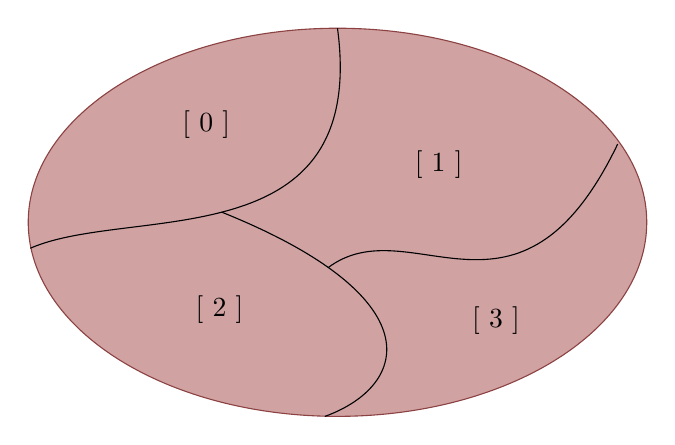
\begin{tikzpicture}[x=0.75pt,y=0.75pt,yscale=-1,xscale=1]
%uncomment if require: \path (0,300); %set diagram left start at 0, and has height of 300

%Shape: Ellipse [id:dp4829810342761349]
\draw  [color={rgb, 255:red, 140; green, 66; blue, 66 }  ,draw opacity=1 ][fill={rgb, 255:red, 208; green, 162; blue, 162 }  ,fill opacity=1 ] (171,152.5) .. controls (171,100.86) and (237.71,59) .. (320,59) .. controls (402.29,59) and (469,100.86) .. (469,152.5) .. controls (469,204.14) and (402.29,246) .. (320,246) .. controls (237.71,246) and (171,204.14) .. (171,152.5) -- cycle ;
%Curve Lines [id:da7772387220169334]
\draw    (172,165) .. controls (220,144) and (335,171) .. (320,59) ;
%Curve Lines [id:da0576638127246778]
\draw    (264.2,147.6) .. controls (366.2,188.6) and (355,231) .. (314,246) ;
%Curve Lines [id:da8789468342677784fig]
\draw    (315.4,174.4) .. controls (355.4,144.4) and (407.4,213.6) .. (455,114.8) ;

% Text Node
\draw (244,97.6) node [anchor=north west][inner sep=0.75pt]   [align=left] {[ 0 ]};
% Text Node
\draw (356,116.8) node [anchor=north west][inner sep=0.75pt]   [align=left] {[ 1 ]};
% Text Node
\draw (250.4,186.4) node [anchor=north west][inner sep=0.75pt]   [align=left] {[ 2 ]};
% Text Node
\draw (383.6,192) node [anchor=north west][inner sep=0.75pt]   [align=left] {[ 3 ]};


\end{tikzpicture}
\caption{Equivalence classes of $\mathbb{Z}$ under the relation $x \equiv y \mod \ 4$}\label{fig:eq-class-zmod4}
\end{figure}

The general idea of quotients based on normalisation may be represented in Typer
without extending the language, with the caveat that the previously mentioned
judgemental equality does not hold. Indeed, this can be done in any language
that supports dependent pairs, as is suggested in\cite[Chap~6.10]{HoTTbook}.
This is unsurprising given that Courtieu's implementation may also be translated
to the Calculus of Inductive Constructions\cite{werner-cic}, a close relative of
Typer. However, the above construction only works when the normalisation
function is idempotent. Further work has then been done by
Cohen\cite{cohen2013pragmatic} to generalise this to normalisation functions
that do not have the same domain and codomain, i.e.\ of type \fn{A $\rightarrow$
  B}. It is also required for such a function to have a right inverse of type
\fn{B $\rightarrow$ A}. In Cohen's work, the first function is known as \id{pi},
i.e.\ the projection into the quotient, whereas the second function is known as
\id{repr}, i.e.\ the representative function.

%% NOTE: I think that maybe its not interesting to show the entire construction,
%% it is sufficient to simply mention the possibility of doing so and direct
%% interested readers to the book for more details

%% We now describe the aforementioned construction in Typer, and then provide a
%% proof that it fulfils the universal property of a quotient.

%% We define a dependent pair as follows (this is why coproducts are related):

%% \begin{minted}[escapeinside=@@,mathescape=true]{haskell}
%% type Sigma (A : Type) (B : A @$\rightarrow$@ Type)
%%   | sigma (fst : A) (snd : B fst);
%% \end{minted}

%% Now, we can define the type $\kw{Qnorm}$ for some type $\id{A}$ and
%% normalisation function $\oftype{r}{A \rightarrow A}$ as a dependent pair that
%% contains some term of type $\id{A}$ and a proof that it has been normalised.
%% This of course requires the idempotency of the normalisation function. We note
%% as well that generally speaking, the codomain of the normalisation function need
%% not be of the same type as its domain, however for the purposes of this
%% construction such a constraint is necessary.

%% \begin{minted}[escapeinside=@@,mathescape=true]{haskell}
%% Qnorm : (A : Type) @$\rightarrow$@ isSet A @$\rightarrow$@ (r : A @$\rightarrow$@ A)
%%         @$\rightarrow$@ (i : (x : A) @$\rightarrow$@ Eq (r (r x)) (r x)) @$\rightarrow$@ Type
%% Qnorm A p r i = Sigma A (@$\lambda$@ (x : A) @$\rightarrow$@ Eq (r x) x)
%% \end{minted}

%% The surjection into $\kw{Qnorm}$ is simply the construction of a dependent pair
%% containing a term that has been normalised and a proof of its normalisation.
%% This is in contrast to the construction that was described previously with
%% $\id{Quotient}$ which applied the normalisation upon the elimination of a
%% quotient, whereas here, normalisation immediately occurs upon the construction
%% of a term of type $\kw{Qnorm}$.

%% We can prove that the equality of $\kw{Qnorm}$ terms is characterised by the
%% equality between the normalised forms of the underlying terms. As usual, we
%% require $\Funapp{\kw{isSet}}{\id{A}}$ to prove this equality. A simple
%% invocation of the \fn{${\Sigma}{\equiv}$\_prop} lemma completes the proof.

%% \begin{minted}[escapeinside=@@,mathescape=true]{haskell}
%% Qnorm_eq : (A : Type) @$\Rrightarrow$@ (x y : A) @$\Rightarrow$@ (p : HoTT_isSet A)
%%            @$\Rightarrow$@ (r : A @$\rightarrow$@ A) @$\Rightarrow$@ (i : (x : A) @$\rightarrow$@ Eq (r (r x)) (r x))
%%            @$\Rightarrow$@ Eq (r x) (r y) @$\rightarrow$@ Eq (Qnorm_in (p := p) (r := r) (i := i) x)
%%                                    (Qnorm_in (p := p) (r := r) (i := i) y)
%% Qnorm_eq = @$\lambda$@ A @$\Rrightarrow$@ @$\lambda$@ x y p r i @$\Rightarrow$@ @$\lambda$@ rx@$\equiv$@ry @$\rightarrow$@
%%   @${\Sigma}{\equiv}$@_prop (B := @$\lambda$@ x @$\rightarrow$@ Eq (r x) x)
%%            (@$\lambda$@ x @$\rightarrow$@ p (r x) x)
%%            (sigma (B := @$\lambda$@ x @$\rightarrow$@ Eq (r x) x) (r x) (i x))
%%            (sigma (B := @$\lambda$@ x @$\rightarrow$@ Eq (r x) x) (r y) (i y))
%%            rx@$\equiv$@ry
%% \end{minted}

%% We can easily prove the reverse of this too, i.e.\ if we have that
%% $\Funapp{\id{Eq}}{(\Funapp{\kw{Qnorm\_in}}{x})}{(\Funapp{\kw{Qnorm\_in}}{y})}$,
%% then $\Funapp{\id{Eq}}{(\Funapp{r}{x})}{(\Funapp{r}{y})}$ is immediate by taking
%% the first projection of the pairs.

%% Finally, we can also show that $\kw{Qnorm}$ fulfils the universal property of a
%% quotient. In other words, we want show the following equivalence:

%% \begin{align*}
%%   & (\Funapp{\kw{Qnorm}}{A}{p}{r}{i} \rightarrow B) \simeq \Sigma \ (A
%%   \rightarrow B) \ (\lambda g \rightarrow (x \ y : A) \rightarrow \Funapp{r}{x}
%%   \equiv \Funapp{r}{y} \rightarrow \Funapp{g}{x} \equiv \Funapp{g}{y})
%% \end{align*}

%% The proof itself is not very interesting as it is largely similar to the proof
%% of the universal property of \id{Quotient} that is provided in
%% \autoref{app:ump-quot} of the appendix. We note however that the reverse
%% direction of this equivalence characterises the elimination principle of
%% $\id{Qnorm}$, as was the case for $\id{Quotient}$.

\section{Cubical Equality and HITs in Cubical Agda}\label{sec:cubical-agda}

Cubical Agda\cite{vezzosi2021cubical} is an extension of the \Agda{} proof
assistant which serves to provide computational meaning to HoTT. This work is
of particular interest to us because of two of its prominent features, cubical
equality and higher inductive types (HITs).

\subsection{Equality} The thing that makes the type theory cubical is its
notion of equality that is represented by functions out of an interval type,
i.e.\ of type \fn{I $\rightarrow$ A}. More specifically, such equality types
are known as \emph{paths} in the literature, an interpretation inspired by
homotopy theory. If an equality between two terms is seen as a path, then we
may construct an equality between two paths to produce a square. This process
may be iterated to produce cubes, hypercubes, etc, justifying the name of the
type theory. Cubical Agda introduced the interval type as a primitive with two
endpoints \fn{i0 :\@ I} and \fn{i1 :\@ I}. Unlike normal types, we are not
allowed to observe the difference between \id{i0} and \id{i1}. This implies
that among other things, pattern matching on an interval variable is
disallowed. The type of homogeneous equality is represented by $\equiv$ with
the following type\footnote{The universe polymorphism of Agda functions is
omitted to simplify the presentation.}:

\begin{minted}[escapeinside=@@,mathescape=true]{agda}
    _@$\equiv$@_ : {A : Set} @$\rightarrow$@ A @$\rightarrow$@ A @$\rightarrow$@ Set
\end{minted}

Readers that are not familiar with \Agda{} are reminded that \fn{\_$\equiv$\_}
means that $\equiv$ is an infix operator\footnote{The underscores indicate
  where the arguments should go, in this case, there should be an argument
  before and after the $\equiv$ operator. Subsequently, we shall use the same
convention when introducing operators.}. We mention as well that parameters
that are within braces are implicit, i.e.\ to be inferred. \id{Set} in Agda is
analogous to Typer's \id{Type}. So if we have two terms \id{x} and \id{y} of
type \id{A}, the type representing a path between the two terms is \fn{x
$\equiv$ y}. In order to construct such an equality, we need to construct a
function \id{f:I $\rightarrow$ A} such that \fn{f i0} is equal to \id{x} and
\fn{f i1} is equal to \id{y}. For example, we construct the reflexive proof of
equality.

\begin{minted}[escapeinside=@@,mathescape=true]{agda}
    refl : {A : Set} {x : A} @$\rightarrow$@ x @$\equiv$@ x
    refl {x = a} = @$\lambda$@ i @$\rightarrow$@ a
\end{minted}

\fn{\{x = a\}} is how we tell \Agda{} that we would like to bind the implicit
argument \id{x} to the variable \id{a} such that it may be used on the
right-hand side. We constructed a constant function that returns \id{a} and
ignores that interval argument \id{i}. This example also illustrates why
explicit pattern matching on \id{i} is not allowed; if we could arbitrarily
assign return values to each endpoint of the interval, we could then prove
equalities between arbitrary terms. To emphasise that the equality proof is
indeed nothing more than a typical function in Agda, we could move the argument
\id{i} to the left-hand side of the equation as would be possible with normal
function arguments.

\begin{minted}[escapeinside=@@,mathescape=true]{agda}
    refl : {A : Set} {x : A} @$\rightarrow$@ x @$\equiv$@ x
    refl {x = a} i = a
\end{minted}

Although pattern matching is forbidden on interval variables, numerous primitives
act on the interval type, allowing us to manipulate them. We illustrate this with
a proof of the commutativity of equality.

\begin{minted}[escapeinside=@@,mathescape=true]{agda}
    comm : {A : Type} {x y : A} @$\rightarrow$@ x @$\equiv$@ y @$\rightarrow$@ y @$\equiv$@ x
    comm p i = p (~ i)
\end{minted}

Like before, we introduced a new interval variable \id{i} since we are
constructing an equality proof which is simply a function. We also make use of
the fact that the proof \id{p} of \fn{x $\equiv$ y} is also a function, hence we
may freely use function application on it. The primitive operator \id{\~{}}
swaps an interval endpoint, the symbol of the operator is inspired by boolean
negation. We can thus verify that \fn{comm p i0 = y} and \fn{comm p i1 = x} as
required.

Having equality proofs that are based on functions out of the interval type also
allows us to derive the theorem of functional extensionality. This theorem says
that functions that are pointwise equal are equal. This is a desirable property
that is not typically provable in Martin-Löf type
theory\cite{martin1975intuitionistic}.

\begin{minted}[escapeinside=@@,mathescape=true]{agda}
    funext : {A B : Type} {f g : A @$\rightarrow$@ B} @$\rightarrow$@ (@$\forall$@ (a : A) @$\rightarrow$@ f a @$\equiv$@ g a) @$\rightarrow$@ f @$\equiv$@ g
    funext p i = @$\lambda$@ x @$\rightarrow$@ p x i
\end{minted}

The proof \id{p} is a witness that the functions \id{f} and \id{g} agree on all
possible input arguments \id{a} of type \id{A}. An example of such a proof could
be constructed for the functions \fn{$\lambda$ x $\rightarrow$ x + 1} and
\fn{$\lambda$ x $\rightarrow$ 1 + x} which are extensionally equal. To prove the
aforementioned theorem, we need to construct a term such that \fn{funext p i0 =
  f} and \fn{funext p i1 = g}. Hence, we construct a lambda function that passes
its argument \id{x} to \id{p} to obtain a proof that \fn{f x $\equiv$ g x}, then
it applies the interval argument \id{i} obtain either \fn{f x} or \fn{g x}.
Summarising the above, \fn{funext p i0 = $\lambda$ x $\rightarrow$ f x} and
\fn{funext p i1 = $\lambda$ x $\rightarrow$ g x}. The $\eta$-equivalence of
functions makes it such that the proof is complete\footnote{For clarity's sake
we did not move the argument \id{x} to the left-hand side of the definition.} as
it implies that \fn{$\lambda$ x $\rightarrow$ f x} is definitionally equal to
\id{f}.

%% The type of paths is the following:

%% \begin{minted}[escapeinside=@@,mathescape=true]{agda}
%% PathP : @$\forall$@ {@$\ell$@} (A : I @$\rightarrow$@ Set @$\ell$@) @$\rightarrow$@ A i0 @$\rightarrow$@ A i1 @$\rightarrow$@ Set @$\ell$@
%% \end{minted}

\subsection{Higher Inductive Types}

Higher inductive types (HITs) are a generalisation of inductive types that has
been popularised by homotopy type theory\cite{HoTTbook}. Aside from the usual
term constructors of inductive types, HITs allow the definition of equality
constructors, i.e.\ equalities between terms of the inductive type. So far,
this is no different from QITs, i.e. the class of quotient types introduced by
Quotient Haskell as was presented in \autoref{sec:related-qit}. What sets HITs
apart from QITs is that HITs allow us to define equalities between equalities,
also known as \emph{higher paths}. In other words, HITs may be seen as a
generalisation of QITs. HITs provide us with an expressive and convenient way
of defining quotients. For instance, we could define the type of integers that
we previously saw\footnote{This definition could have benefited from another
constructor that produces a proof that all equality proofs between two
integers are themselves equal. This is known as the set truncation of the
type. We decided not to do it however as higher paths are not immediately
relevant to our work}.

\begin{minted}[escapeinside=@@,mathescape=true]{agda}
    data Int : Type where
      zero : Int
      pred : Int @$\rightarrow$@ Int
      succ : Int @$\rightarrow$@ Int
      predsucc@$\equiv$@id : (n : Int) @$\rightarrow$@ pred (succ n) @$\equiv$@ n
      succpred@$\equiv$@id : (n : Int) @$\rightarrow$@ succ (pred n) @$\equiv$@ n
\end{minted}

Here we define a new type \id{Int}. The first three constructors are known as
\emph{term constructors} and are no different from the constructors that one
defines with normal inductive types. While defining the term constructors, we
may simultaneously define equality constructors\footnote{They are more commonly
known as path constructors in a HoTT setting.} between terms of the inductive
type. The \id{predsucc$\equiv$id} constructor says that for any integer \id{n},
we may construct a proof of (propositional) equality between \fn{pred (succ n)}
and \id{n}, ditto for \id{succpred$\equiv$id}. Not only can we prove such
equalities, but they also have to be respected during elimination. Equality
constructors have to be handled as separate branches when we carry out case
analysis. We illustrate this by constructing a function that negates integers by
recursively switching every \id{pred} to a \id{succ} and vice versa.

\begin{minted}[escapeinside=@@,mathescape=true]{agda}
    Int-negate : Int @$\rightarrow$@ Int
    Int-negate zero = zero
    Int-negate (pred n) = succ (Int-negate n)
    Int-negate (succ n) = pred (Int-negate n)
    Int-negate (predsucc@$\equiv$@id n i) = succpred@$\equiv$@id (Int-negate n) i
    Int-negate (succpred@$\equiv$@id n i) = predsucc@$\equiv$@id (Int-negate n) i
\end{minted}

In the first three branches, we say what the function should do to the term
constructors. The last two branches are proof that the function behaves
coherently with respect to the two equality constructors of $\id{Int}$.
According to \fn{predsucc$\equiv$id n}, we know that \fn{pred (succ n)} and
\fn{n} are supposed to be equal. By congruence of equality, the application of
\id{Int-negate} to both sides of this equality should again yield two equal
terms, i.e.\ \fn{succ (pred (Int-negate n))} and \fn{Int-negate n} should be
equal. We can easily construct a proof of this equality by using the term
\fn{succpred$\equiv$id (Int-negate n)}. The other branch that deals with
\fn{succpred$\equiv$id n} may be handled similarly.

\subsubsection{Quotient Types as a HIT}\label{subsec:quot-as-hit}

We could also define quotient types as formulated by
Hoffman\cite{hofmann1995extensional} as a higher inductive type in \Agda{}.

\begin{minted}[escapeinside=@@,mathescape=true]{agda}
    data _/_ (A : Type) (R : A @$\rightarrow$@ A @$\rightarrow$@ Type) : Type
       where
       [_] : A @$\rightarrow$@ A / R
       eq/ : (a b : A) @$\rightarrow$@ (r : R a b) @$\rightarrow$@ [ a ] @$\equiv$@ [ b ]
\end{minted}

We define the quotient type former \fn{\_/\_} which has two parameters. \id{A}
is the base type of the quotient, and \id{R} a binary relation defined on the
type \id{A}. \fn{[\_]} is a mixfix operator that acts as the only term
constructor of the quotient type; conceptually it acts as the projection of a
term of the base type into the quotient. \fn{eq/} on the other hand is an
equality constructor that says that if we can provide a witness of \fn{R a b},
i.e.\ a proof that terms \id{a} and \id{b} fulfil the underlying relation of the
quotient, then their projections into the quotient are also equal.

To illustrate how this works, we present an example of a quotient type in the
form of unordered pairs. The type of pairs is \fn{A $\times$ B} and its terms
have the form \fn{(x , y)}. The concept of unordered pairs is such that \fn{(x ,
  y)} should be equal to \fn{(y , x)}. We thus define a relation on the type of
pairs such that permutations of the elements are equivalent.

\begin{minted}[escapeinside=@@,mathescape=true]{agda}
UPairR : @$\forall$@ {l} {A : Type} @$\rightarrow$@ A @$\times$@ A @$\rightarrow$@ A @$\times$@ A @$\rightarrow$@ Type
UPairR (x1 , y1) (x2 , y2) = ((x1 @$\equiv$@ x2) @$\times$@ (y1 @$\equiv$@ y2)) @$\uplus$@ ((x1 @$\equiv$@ y2) @$\times$@ (y1 @$\equiv$@ x2))
\end{minted}

$\uplus$ is the type theoretical equivalent of disjunction. We say that two
pairs are equivalent if they are equal element-wise or if by swapping the second
pair we get element-wise equality. With that, we can now define the type of
unordered pairs.

\begin{minted}[escapeinside=@@,mathescape=true]{agda}
    UnorderedPair : Type @$\rightarrow$@ Type
    UnorderedPair A = (A @$\times$@ A) / UPairR
\end{minted}

If we would like to define a map from \fn{UnorderedPair A} to some type \id{B},
intuitively speaking we would require some function \id{f} of type \fn{A
  $\times$ A $\rightarrow$ B} such that it is a commutative function so that the
ordering of the pairs does not matter, i.e.\ that \fn{$\forall$ x y. f x y
  $\equiv$ f y x}. Indeed, we can define the function \id{UPairR-elim} that
captures the above idea.

\begin{minted}[escapeinside=@@,mathescape=true]{agda}
    UPairR-elim : @$\forall$@ {A B} @$\rightarrow$@ (f : A × A @$\rightarrow$@ B)
                @$\rightarrow$@ ((x y : A) @$\rightarrow$@ f (x , y) @$\equiv$@ f (y , x))
                @$\rightarrow$@ UnorderedPair A @$\rightarrow$@ B
    UPairR-elim f h [ p ] = f p
    UPairR-elim f h (eq/ (x1 , y1) (x2 , y2) r i) = ?
\end{minted}

Pattern matching on an unordered pair gives us two cases to cover. The \id{[\_]}
constructor is handled easily as we simply pass the pair \id{p} to the function
\id{f}. The branch for the equality constructor on the other hand is more
interesting. The placeholder needs to be equal to \fn{f (x1 , y1)} when \fn{i =
  i0} and it needs to be \fn{f (x2 , y2)} when \fn{i = i1}, in other words we
need to construct an equality between \fn{f (x1 , y1)} and \fn{f (x2 , y2)} and
apply \id{i} to it. Here is a sketch of the proof: it may be constructed by
doing case analysis on \id{r}, a term of type \fn{UPairR (x1 , y1) (x2 , y2)}.
In the case of the left injection into the disjunction, we prove the required
equality using the congruence property of equality; in the other case, we just
cast \fn{h x1 y1} to the required type.

\section{Setoid Rewriting}

Quotient types are not provided as a primitive in the \Coq{} proof assistant.
To explain how quotient types are emulated in \Coq{}, we briefly introduce the
rewriting mechanism of \Coq{}, implemented in the form of the \kw{rewrite}
tactic. Instead of constructing a proof term from scratch by hand to prove a
theorem as we have seen so far, tactics allow us to transform the goal, i.e.
what we need to show to prove a theorem, into smaller or easier to prove
subgoals. For instance, if we had \fn{A $\wedge$ B} as a goal to prove, we
could use a tactic to split it into 2 subgoals, i.e. \id{A} and \id{B},
allowing to prove them separately. Tactics also allow us to manipulate
hypotheses. Suppose instead that we have the hypothesis that \fn{A $\wedge$ B}
is true, we may use a tactic to split it into two separate hypotheses. If we
have a certain proof goal that requires us to produce a term of type \fn{m + n
$\le$ n + m} and we have proof that \fn{m + n $\equiv$ n + m}, we may use the
\kw{rewrite} tactic in to rewrite the goal such that it becomes \fn{n + m $\le$
n + m}. The simplified goal may thus be easily proven using the reflexivity
property of $\le$. Every construction is congruent with respect to the equality
type, hence rewrites using the equality type may be carried out in any context,
however, this is not true of setoid rewriting as we shall discuss below.

Plain rewriting allows rewriting with \emph{equal} terms, generalised
rewriting\cite{sozeau2009new, coq-gen-rewriting} on the other hand enables
rewriting using terms that are \emph{related} by some binary relation, often
represented as a function of type \fn{A $\rightarrow$ A $\rightarrow$
  \kw{Prop}}\footnote{\kw{Prop} is \Coq{}'s universe of proof irrelevant
propositions.}. Unlike equality, this form of rewriting does not work in all
contexts, instead, it only works in contexts that are compatible with the
relation. A base type \id{A} equipped with an equivalence relation that is meant
to behave as an equality characterises a structure known as a
setoid\cite{hofmann1995simple}. Instead of constructing a new type to represent
the quotient of the base type, we would directly work with the base type.
Suppose that we had a proof of \fn{a R b} where \id{R} is an infix binary
relation, we would be able to rewrite \id{a} to \id{b} if the context of \id{a}
in the goal is compatible with the relation. However, every function definition
that interacts with the setoid needs to be accompanied by proof that setoid
equivalence is respected. This is in contrast to the ideal situation where such
coherence proofs are required \emph{only} in the function that eliminates
quotients, subsequent interaction and composition of this function should be
free of the burden of such proof obligations. The generalised rewriting approach
has historically been the go-to way of modelling quotient types in \Coq{},
however, such an approach is known to be rather laborious. This phenomenon is
often designated as \emph{setoid hell} by the community\footnote{Examples of
community discussions on this topic may be found at
\url{https://stackoverflow.com/questions/65493694/why-do-calculus-of-construction-based-languages-use-setoids-so-much/}
and
\url{https://proofassistants.stackexchange.com/questions/908/what-exactly-is-setoid-hell/}}.
Although \Coq{} offers numerous tactics to facilitate the usage of setoids, it
quickly becomes unwieldy in the case of large programs.

\section{Quotients in Lean}\label{sec:intro-lean-quotients}

Lean implements quotients by providing the below set of primitives in the core
library\footnote{Like before, we omit universe polymorphism to simplify the
presentation.}.

%% SM: Curious!  So they don't have an axiom that reflects the expected
%% reduction rule, like `Quot.lift f (Quot.mk x) = f x`?
\begin{minted}[escapeinside=@@,mathescape=true]{lean}
    opaque Quot {A : Sort} (r : A @$\rightarrow$@ A @$\rightarrow$@ Prop) : Sort

    opaque Quot.mk {A : Sort} (r : A @$\rightarrow$@ A @$\rightarrow$@ Prop) (a : A) : Quot r

    opaque Quot.lift {A : Sort} {r : A @$\rightarrow$@ A @$\rightarrow$@ Prop} {B : Sort} (f : A @$\rightarrow$@ B) :
      (@$\forall$@ a b : A, r a b @$\rightarrow$@ f a = f b) @$\rightarrow$@ Quot r @$\rightarrow$@ B

    opaque Quot.ind {A : Sort} {r : A @$\rightarrow$@ A @$\rightarrow$@ Prop} {B : Quot r @$\rightarrow$@ Prop} :
      (@$\forall$@ a : A, B (Quot.mk r a)) @$\rightarrow$@ @$\forall$@ q : Quot r, B q

    axiom Quot.sound : @$\forall$@ {A : Sort} {r : A @$\rightarrow$@ A @$\rightarrow$@ Prop} {a b : A}, r a b
      @$\rightarrow$@ Quot.mk r a = Quot.mk r b
\end{minted}

Lean has two universes of types, \kw{Prop} and \kw{Type}. \kw{Type} is analogous
to its counterpart in Typer as explained in \autoref{subsec:typer-comparison}.
\id{Prop}, on the other hand, is \Lean{}'s universe of proof-irrelevant
%% SM: Really?  My understanding was that Lean had propositional
%% proof irrelevance via an axiom, rather than definitional
%% proof irrelevance.  Hmm... it looks like you're right they made it
%% definitional in Lean 4, tho I don't know the detail of how they did it.
propositions. This implies that all proofs of a proposition are definitionally
equal. When we annotate a type to be of the universe \kw{Sort}, we are
essentially saying that it could belong to either \kw{Prop} or
\kw{Type}\footnote{Again, we provide a simplistic description of how things
really are.}. \kw{opaque} definitions are not expanded during simplification or
reduction, this may be seen as a means of abstraction to keep the internal
structure of a definition hidden. Lean also allows us to define \kw{axiom}s;
%% SM: Check all your uses of "only" which tend to be on the ambiguous
%% side.  Instead of "may only be used for" you should say "may be used only
%% for".  Yes, it's a very common (and hence minor) misuse.
they may be seen as variables without a concrete definition and may be
used only for for type-checking purposes.

First, they introduce the \id{Quot} type former, parametrised by some type
\id{A} and a binary relation on \id{A}. \id{Quot.mk} is the term former that
takes a term \fn{a :\@ A} and constructs a quotient term out of it. In contrast
to Cubical Agda that supports the elimination of quotients through direct
pattern-matching, \Lean{} provides two functions \id{Quot.lift} and
\id{Quot.ind} for normal elimination and dependent elimination respectively.
\id{Quot.lift} works in a similar way to how we did pattern matching on a
quotient type in \autoref{subsec:quot-as-hit}. To eliminate a quotient term, we
need to provide three things: first, a function that takes a term of type
\id{A} to some type \id{B}; second, proof that this function maps equivalent
terms of type \id{A} (based on the underlying relation) to equal outputs; and
third, the quotient term that we wish to eliminate.

The dependent eliminator \id{Quot.ind} is more interesting. The elimination
motive \id{B} is a family of propositions, implying that we are not allowed to
eliminate a quotient term to a type that lives in \kw{Type}. \id{Quot.ind}
expects a dependent function that takes a term \id{a} of type \id{A} and maps
it to \fn{B (Quot.mk a)}. Unlike \id{Quot.ind}, we do need to provide a proof
that this function respects the underlying relation since we are eliminating to
%% Suppose that we had r a b, then we can cast `f a` from `B (Quot.mk a)` to
%% `B (Quot.mk b)`, and since this type is a subsingleton, what we obtain will
%% necessarily be equal to `f b`.
\kw{Prop}. The \id{Quot.sound} axiom is the essence of quotient types, it
states that \id{Quot.mk} maps `related' terms to equal terms in the quotient.
It is comparable with the \id{eq/} constructor described in
\autoref{subsec:quot-as-hit}.

However, Lean's quotient types have a few shortcomings. The introduction of
axioms tends to block computation; that is, it breaks a desirable property of
type theory known as canonicity\cite{hofmann1995extensional}, which states that
every term in a closed context may be reduced to a canonical form. A term is of
canonical form if it is built up using only the constructors of its type. Using
\id{Bool} as an example, a closed term \fn{b :\@ Bool} must be able to be
reduced to either \id{true} or \id{false}. Type casts using equality proofs
that are axioms such as \id{Quot.sound} result in \emph{stuck terms}. Another
problem arises when we take the quotient of a \kw{Prop}. Such a construction is
not very meaningful as all proofs of a proposition are already definitionally
equal in \Lean{}, however, it is nevertheless allowed. This has been shown to
break subject reduction\cite{carneiro-lean-type-theory}, i.e., if we have a
term \fn{t :\@ A}, and \id{t} reduces to \id{u}, it might be the case that
\id{u} is not of type \id{A}, or worse, \id{u} may not even type-check. Our
implementation of quotients shares similarities with \id{Lean}; however, we aim
to circumvent the aforementioned problems.

\section{Quotients in Observational Type Theory (TT$^{obs}$)}

%% TODO: Be a bit more careful with this section as I'm reading about this for
%% the first time, so I might be prone to misunderstanding the article
%% (pujet2022observational)

We discuss how quotients may be implemented in observational type theory, more
specifically in TT$^{obs}$\cite{pujet2022observational}. We note, however, that
we do not have a programming language or proof assistant implemented based on
observational type theory to date. Hence, this discussion is on the addition of
quotients to TT$^{obs}$ on a theoretical level, readers who are not interested
in this should feel free to skip this section. In TT$^{obs}$, every type has a
built-in setoid structure which is preserved by all terms by construction.
Equality is represented by the setoid equality of types themselves, each type
is thus free to have its own notion of equality. The observational equality
type is denoted as \fn{t $\sim_A$ u}, this type represents the equality of
terms \id{t} and \id{u} at type \id{A}. However, this is not a typical type
former of equality types as we have previously seen, $\sim$ in reality pattern
matches on the type \id{A} and the two endpoints and computes to a type. We
show two typing rules to illustrate this point. First, we show the rule for
observational equality between two propositions. Note that in TT$^{obs}$,
$\Omega_i$ is the i$^{th}$ universe of proof irrelevant propositions. Readers
who are unfamiliar with natural deduction may consult
\autoref{app:natural-deduction} for a short introduction. Note, however, that
in this subsection, we make use of an additional type of judgement in the form
of $\oftype{\ctx}{t \Rightarrow{} u}{A}$. This judgement states that the
%% SM: Don't presume the reader knows what means "t reduces to u at type A".
term \id{t} reduces to \id{u} at type \id{A} in context $\ctx$, in other words,
term \id{t} of type \id{A} reduces to some other term \id{u} of the same type
in the given context.

\begin{prooftree*}
  \hypo{\oftype{\ctx}{A}{\Omega_i}}
  \hypo{\oftype{\ctx}{B}{\Omega_i}}

  \infer2[\kw{EQ-$\Omega$}]{\oftype{\ctx}{A \sim_{\Omega_i} B \Rightarrow{} (A
      \rightarrow{} B) \wedge{} (B \rightarrow{} A)}{\Omega_i}}
\end{prooftree*}

Observational equality between propositions is simply represented by their
logical equivalence, implying that propositional extensionality is baked into
the theory. Next, we discuss the reduction rule for observational equality
between functions.

\begin{prooftree*}
  \hypo{\oftype{\ctx}{f}{\Pi{} (x:A).B}}
  \hypo{\oftype{\ctx}{g}{\Pi{} (x:A).B}}

  \infer2[\kw{EQ-FUN}]{\oftype{\ctx}{f \sim_{\Pi{} A B} g \Rightarrow{}
      \Pi{} (x:A). \Funapp{f}{x} \sim_B \Funapp{g}{x} }{\Omega_i}}
\end{prooftree*}

We observe that observational equality between functions simply reduces to a
proof of pointwise equality of these functions, in other words, functional
extensionality is also built into the system.

All that to say this system lends itself well to the introduction of quotient
types. The quotient type \fn{A/R} is interpreted as a setoid with \id{A} as its
base type and the relation \id{R} as its setoidal equality. This of course
requires the relation \id{R} to be reflexive, symmetric, and transitive. In the
theory, equality between two terms that are projections into the quotient
(syntactically represented by $\pi(t)$) reduces to the underlying relation
between the base terms, as is illustrated by the following rule:

%% SM: This OITT section should maybe be a bit more careful to compare OTT
%% to your work (and a bit less about presenting OTT in general).
%% The rule below is directly relevant, which is good.
%% But what's missing is for example what the elimination form looks like.

%% NOTE: I want to aggressively summarise this section, and maybe mention it
%% again at the very end (i.e. not in this related works section that's going to
%% the front). Especially since all this is theoretical and hasn't really been
%% realised in a real proof assistant yet. For now, too many explanations need
%% to be given in order for readers to be able to make sense of this

\begin{prooftree*}
  \hypo{\oftype{\ctx}{t}{A}}
  \hypo{\oftype{\ctx}{u}{A}}

  \infer2{\oftype{\ctx}{\pi(t) \sim_{A/R} \pi(u) \Rightarrow{} \Funapp{R}{t}{u}
    }{\Omega_i}}
\end{prooftree*}

The fact that quotient equality shares the representation as the underlying
relation has interesting implications. This means that when we have a term of
type \fn{R t u}, the same term also doubles as a proof of equality between the
projections of \id{u} and \id{t} into the quotient, as opposed to other systems
such as Cubical Agda where such a proof would need to be constructed using a
dedicated constructor. Consider the (dependent) elimination rule of quotients:

\begin{prooftree*}
  \hypo{\oftype{\ctx}{B}{A/R \rightarrow U}}
  \hypo{\oftype{\ctx}{t_\pi}{\Pi (x: A). \Funapp{B}{\pi(x)}}}
  \hypo{\oftype{\ctx}{u}{A/R}}
  \infer[no rule]3{\oftype{\ctx}{t_{\sim{}}}{\Pi(x,y : A).\Pi(e : \Funapp{R}{x}{y}). (\Funapp{t_\pi}{x}) \sim_{\Funapp{B}{\pi(x)}} \kw{cast}(\Funapp{B}{\pi(y)}, \Funapp{B}{\pi(x)}, \Funapp{B}{e^{-1}}, \Funapp{t_\pi}{y})}}

  \infer1{\oftype{\ctx}{\Funapp{\kw{Q-elim}}(B, t_\pi, t_\sim, u)}{\Funapp{B}{u}}}
\end{prooftree*}

\id{t$_\pi$} is the function that gets to act on the term of the base type, not
unlike what we require in other implementations of quotients that we have seen.
\id{t$_\sim$}, the proof that \id{t$_\pi$} respects the quotient, is stated
somewhat differently from ours because of how quotient equality works in this
setting. We require a proof that \fn{t$_\pi$ x} is equal to \fn{t$_\pi$ y} cast
to the same type as the former, i.e.\ from \fn{B $\pi$(y)} to \fn{B $\pi$(x)}.
The third argument of \kw{cast} is a witness that the two types are equal. Since
\id{e} is a term of type \fn{R x y}, it is effectively a proof of \fn{$\pi$(t)
  $\sim_{A/R}$ $\pi$(u)}. \fn{B e$^{-1}$} is thus the functorial action of
\id{B} on the inversion of the equality proof \id{e}, in other words, this is
the application of the congruence property of equality.

\chapter{Cubical Equality and Quotient Types}
%% SM: It's probably a good place to talk about (as a kind of self-reflection)
%% the fact that your thesis on "quotient types in Typer" talks almost
%% more about equalities than about quotients.

This chapter starts by presenting cubical equality along with our adaptation of
it to Typer. We then build on that to discuss how we implemented quotient types
in Typer.

\section{Cubical Equality}\label{sec:cubical-equality}

We first present the existing version of Typer's equality type before presenting
our implementation of cubical equality in Typer. This is done notably to
familiarise readers with Typer's equality in general and to highlight the
advantages of cubical equality in subsequent sections. Then, we present the
typical definition of the \emph{interval type} defined as a higher inductive
type as can be found in various sources such as the HoTT
book\cite[Chap~6.3]{HoTTbook}, a recent work that describes the fundamental
concepts of HoTT and innovations in mathematics made possible by univalent
foundations. We subsequently present our alternative formulation of the interval
type and show that it is equivalent to the traditional definition. Finally, we
define \emph{cubical equality}, a different take on the equality type, based on
the aforementioned interval type.

\subsection{Typer's Equality Type}\label{sec:typer-old-eq}

Typer's primitive equality type is similar to that defined in Martin-Löf
intensional type theory\cite{martin1975intuitionistic} (ITT) such that the
equality is homogeneous and that equality reflection is not supported. Its type
former takes on the following form:

\begin{minted}[escapeinside=@@,mathescape=true]{agda}
Eq : (A : Type) @$\Rrightarrow$@ A @$\rightarrow$@ A @$\rightarrow$@ Type
\end{minted}

Its one and only term constructor is none other than the reflexivity constructor.

\begin{minted}[escapeinside=@@,mathescape=true]{agda}
Eq_refl : (x : ?A) @$\Rrightarrow$@ Eq x x
\end{minted}

As mentioned in the introduction, two equal things may be substituted for one
another according to the principle of the indiscernibility of identicals, also
known as Leibniz's law. This essentially means that a property that is true of
one type would necessarily also be true of another type that is equal to it. If
we are working in the realm of natural numbers, we could construct predicates
such as ``x is an even number'', ``x is greater than zero'' etc. In the spirit
of the Curry-Howard correspondence, such predicates would be represented by type
families. For instance, we could define the type family \id{Even} such that for
any natural number \id{m}, a term of type \fn{Even m} is a proof that \id{m} is
even. Naturally, if we know that \id{m} and \id{n} are equal and that \id{m} is
even, we should also be able to derive the fact that \id{n} is also even. The
\emph{cast} operation allows us precisely to do the above. We define the
primitive \id{Eq\_cast} such that it takes a proof that \id{x} and \id{y} of
type \id{A} are equal, a type family \fn{f :\@ A $\rightarrow$ Type} and
gives us a function that maps \fn{f x} to \fn{f y}.

\begin{minted}[escapeinside=@@,mathescape=true]{agda}
    Eq_cast : (x y : ?A) @$\Rrightarrow$@ (p : Eq x y) @$\Rrightarrow$@ (f : ?A @$\rightarrow$@ Type) @$\Rrightarrow$@ f x @$\rightarrow$@ f y
\end{minted}

It has the following reduction rule:

\begin{prooftree*}
  \hypo{\id{p} \simeq{} \id{Eq\_refl}}
  \infer1{\Funapp{\id{Eq\_cast}}{\id{x}}{\id{y}}{\id{p}}{\id{f}}{\id{fx}} \leadsto{} \id{fx}}
\end{prooftree*}

\id{Eq\_cast} only reduces when the equality proof passed to it is the
reflexivity proof. To illustrate how \id{Eq\_cast} may be used, we derive a
property of the equality type, namely the commutativity of equality, i.e.\ if
\id{x} is equal to \id{y}, then \id{y} is naturally also equal to \id{x}.

\begin{minted}[escapeinside=@@,mathescape=true]{agda}
    Eq_comm : (x y : ?A) @$\Rrightarrow$@ Eq x y @$\rightarrow$@ Eq y x
    Eq_comm p = Eq_cast (f := @$\lambda$@ a @$\rightarrow$@ Eq a x) (p := p) Eq_refl
\end{minted}

To prove this, we use \id{Eq\_cast} with an elimination motive that is an
equality with its right-hand side fixed to be \id{x}, whereas its left-hand side
is free to vary. By passing it the proof \id{p} that \id{x} is equal to \id{y},
we are left with a function that maps \fn{Eq x x} to \fn{Eq y x}, thus we pass
it a proof of reflexivity that \id{x} is equal to itself to obtain what we
require.

\subsection{Interval type}\label{sec:interval-introduction}

In this section, we base our definitions on the assumption that we have an
existing equality type similar to what was described in the previous subsection,
i.e.\ that we have a type former \fn{\_$\equiv$\_ :\@ A $\rightarrow$ A
  $\rightarrow$ Type} along with its constructor and eliminator. We assume that
we have access to the following syntax in the subsequent discussion.

\setlength{\grammarparsep}{20pt plus 1pt minus 1pt} % increase separation between rules
\setlength{\grammarindent}{4em} % increase separation between LHS/RHS

%% The `renewcommands` make the angle brackets go away
\renewcommand{\syntleft}{}
\renewcommand{\syntright}{}
\begin{grammar}
<$T$> ::= \ldots
\alt{} \fn{$T_{x}$ $\equiv$ $T_{y}$}
\alt{} \fn{\kw{refl}$_{T_x}$}
\alt{} \fn{\kw{cong}$_{T_f}$(${T_p}$)}
\alt{} \fn{\kw{cast}($T_{p}$, $T_{f}$, $T_{fx}$)}
\end{grammar}

A new addition here is \kw{cong} which refers to the congruence property of
equality, if we have a proof \id{p} of \fn{x $\equiv$ y} and some function
\id{f}, then $\kw{cong}_f(p)$ constructs a proof of \fn{f x $\equiv$ f y}.

This helps us to introduce the interval type and its relationship to the
equality type. We will ultimately define a new equality type that will then form
the backbone of the rest of this work.

\begin{center}
  \begin{prooftree}
      \infer0{\oftype{\ctx}{\bI}{\kw{Type}}}
  \end{prooftree}
  \qquad
  \begin{prooftree}
      \infer0{\oftype{\ctx}{i_{0}}{\bI}}
  \end{prooftree}
  \qquad
  \begin{prooftree}
      \infer0{\oftype{\ctx}{i_{1}}{\bI}}
  \end{prooftree}
  \qquad
  \begin{prooftree}
      \infer0{\oftype{\ctx}{\id{seg}}{\eqtype{i_0}{i_1}}}
  \end{prooftree}
\end{center}

We postulate the existence of the interval type $\bI$, along with its endpoints
\id{$i_0$} and \id{$i_1$}. The intuition is that elements of $\bI$ correspond
to points in the real unit interval $[0, 1]$. We also have \id{seg} which is a
witness of equality between \id{$i_0$} and \id{$i_1$}, or more specifically, a
continuous path between them. The path connecting the two endpoints represents
the continuum of points between them, analogous to the real interval which
consists of all real numbers between 0 and 1.

The elimination of $\bI$ is similar to that of \id{Bool} as described in
\autoref{subsec:intro-fn-ind-types}, the only difference is that we also need
to prove that $\id{seg} : \eqtype{i_0}{i_1}$ is respected. We define the
elimination principle of $\bI$ using the \fn{elim$_{\bI}^{A}$ (M, N, P, i)}
syntax. $A$ is the \emph{motive} of the elimination, i.e.\ the type we wish to
eliminate to. \id{M} and \id{N} are what we would like the output of the
elimination to be when \id{i} is equal to $\ileft$ and $\iright$ respectively,
this is analogous to what we would place in the \kw{then} and \kw{else}
branches during \id{Bool} elimination. \id{P} is a proof that \id{M} and
\id{N} are equal, thus ensuring that the elimination is coherent. More
formally, the typing rule of the elimination rule may be stated as follows:

\begin{prooftree*}
   \hypo{\oftype{\ctx}{M}{A}}
   \hypo{\oftype{\ctx}{N}{A}}
   \hypo{\oftype{\ctx}{P}{\eqtype{M}{N}}}
   \infer3{\oftype{\ctx, \oftype{i}{\bI}}{\kw{elim}_{\bI}^{A} (M, N, P, i)}{A}}
\end{prooftree*}

It has the below computation rules:

\begin{align*}
  & \kw{elim}_{\bI}^{A}(M, N, P, \ileft) \leadsto{} M \\
  & \kw{elim}_{\bI}^{A}(M, N, P, \iright) \leadsto{} N \\
  & \kw{cong}_{\kw{elim}_{\bI}^{A}(M, N, P)}(\id{seg}) \leadsto{} P
\end{align*}

We can expect the first two rules to hold definitionally. Definitional equality
of two terms is determined by expanding out definitions. So when we say that
$\kw{elim}_{\bI}^{A}(M, N , P, \ileft)$ is definitionally equal to \id{M}, we
are saying that the former reduces to the latter when we check for equality. If
we imagine that the first two computation rules were defined via
pattern-matching, it would make sense for these equations to hold
definitionally. The third rule is a more curious case, by the congruence of
equality, the application of the interval eliminator with the equality proof
$\id{P}$ to $\id{seg}$ should yield an equality proof between $\id{M}$ and
$\id{N}$. The rule suggests that this should compute to $\id{P}$ itself. From a
computational point of view, equalities between equality proofs are only an
important consideration in a proof-relevant setting, e.g.\ in the context of
HoTT\@. While working in synthetic homotopy theory, which is where the interval
type is often used, such a rule is deemed as natural and necessary. Since this
is not directly related to our work, we shall not further justify this rule. In
most cases, this rule does not hold definitionally as the \kw{cong} construct is
defined independently and it would be highly unusual to separately define how it
should compute on new constructs such as the interval type. In cases where we
are unable to make the third rule hold definitionally, we usually then postulate
a propositional equality between $\kw{cong}_{\kw{elim}_{\bI}^{A}(M, N,
  P)}(\id{seg})$ and P.

To provide an intuition for what $\bI$ is like, we use the eliminator to
construct a map from $\bI$ to \id{Bool}. For instance, two maps that we may
construct are $\lambda \id{i} \rightarrow \kw{elim}_{\bI}^{Bool}(\id{true},
\id{true}, \kw{refl}_{true}, \id{i})$ and $\lambda \id{i} \rightarrow
\kw{elim}_{\bI}^{A}(\id{false}, \id{false}, \kw{refl}_{\id{false}}, \id{i})$.
The proof term that is required by the eliminator forces us to map $\ileft$ and
$\iright$ to two equal terms. We would not be able to use the
eliminator to map $\ileft$ and $\iright$ to \id{true} and \id{false}
respectively as the type \fn{true $\equiv$ false} is uninhabited.

\subsection{Motivation}
We show that a function with an interval argument returning some type \id{A},
i.e.\ a function with type \fn{$\bI \rightarrow A$} is equivalent to an equality
proof between two terms of type \id{A}. To build an intuition as to why this
might be true, consider a \id{Bool} type where \id{true} and \id{false} are
indistinguishable. Then a function with this \id{Bool} type as an argument is
necessarily constant on its argument. Suppose that we have such a function named
\id{h}, we thus have a witness of the equality of \fn{h $\ileft$} and \fn{h
  $\iright$}.

In order to state the aforementioned theorem, we first introduce dependent
pairs. We use the usual syntax to denote the type of dependent pairs,
i.e.\ $\Sigma_{\oftype{x}{A}}. B$. Here, the first projection of type \id{A} and
is named \id{x}; the type of the second projection, \id{B} may depend on the
term \id{x}. Terms of dependent pairs have the following form $\braket{a, b}$.
Now, we formally state the theorem that we are interested in.

\begin{theo}\label{theo:i->a-equiv}
The following type is inhabited:

\begin{align}
  % & \bI \rightarrow A \ \simeq \ \Sigma_{\oftype{x}{A}} . \Sigma_{\oftype{y}{A}} . \eqtype{x}{y}\nonumber
  & \bI \rightarrow A \ \ \simeq \ \ \sum\limits_{(\oftype{x}{A})} \sum\limits_{(\oftype{y}{A})} \eqtype{x}{y}\nonumber
\end{align}

\end{theo}

$\sum\limits_{(\oftype{x}{A})} \sum\limits_{(\oftype{y}{A})}
\eqtype{x}{y}\nonumber$ may be seen as a triplet containing two terms of type
\id{A} along with a proof of their equality. We provide a proof of the above in
Appendix~\ref{app:proof-i->a-equiv}. By establishing the above equivalence, we
no longer require the \fn{_$\equiv$_} type former that we assume we had in
\autoref{sec:interval-introduction} as we may represent the equality type using
functions out of the interval.

\subsection{Adaptation to Typer}\label{sec:eq-justification}

We have established in the previous section that equality between two terms is
equivalent to a function out of the interval. Its defining characteristic is
that the output of such a function has to agree at both endpoints of $\bI$.
This is enforced by the elimination principle of the $\bI$ that ensures that
\id{seg} is respected. An alternate way of enforcing this is by using functions
with erasable arguments out of a $\mathbbm{2}$-type, i.e.\ a type with two
distinct constructors that take no arguments, such as the \id{Bool} type.
Recall that an argument that is marked as erasable has no computational role
during run time, as explained in \autoref{sec:intro-typer}. In other words, we
can first define the interval type as a normal inductive data type. Next, we
model the equality type as a function with an erasable argument out of the
interval type.

\begin{minted}[escapeinside=@@,mathescape=true]{agda}
    type I
      | @$i_0$@
      | @$i_1$@
\end{minted}

More concretely, we define a function with the following type:

\begin{minted}[escapeinside=@@,mathescape=true]{agda}
    h : I @$\Rrightarrow$@ A
\end{minted}

Intuitively, since \id{h} is not allowed to use its argument in a
computationally relevant manner, what it returns when passed $i_0$ and $i_1$
must be the same. With that, we can postulate the following equivalence.

\begin{align*}
  & \bI \Rrightarrow A \ \ \simeq \ \ \sum\limits_{(\oftype{x}{A})} \sum\limits_{(\oftype{y}{A})} \eqtype{x}{y}\nonumber
\end{align*}

The above shall be the basis of our new definition of equality types.

\subsection{Manipulation of the Interval type}\label{sec:interval-manipulation}

We introduce a few primitive operations on the interval type whose usefulness
will become clear after we introduce our version of the equality type that is
based on the interval type. When providing the reduction rules for these
operations, we omit the congruence rules for brevity. Readers who are
unfamiliar with the syntax of these rules are referred to
\autoref{app:reduction-rules}.

\subsubsection*{Negation}

The negation operator does what its name suggests, i.e.\ it simply negates or
swaps endpoints of the interval type. Unsurprisingly, it has the following type:

\begin{minted}[escapeinside=@@,mathescape=true]{agda}
    I_not : I @$\rightarrow$@ I
\end{minted}

The negation operator computes as follows:

\begin{mdframed}[nobreak=true]
  \begin{center}
    \begin{prooftree}
        \infer0[\textsc{I-Not$_1$}]{\Funapp{\fn{I\_not}}{i_0} \leadsto{} i_1}
    \end{prooftree}
    \qquad
    \begin{prooftree}
        \infer0[\textsc{I-Not$_2$}]{\Funapp{\fn{I\_not}}{i_1} \leadsto{} i_0}
    \end{prooftree}

    \hfill \break

    \begin{prooftree}
        \infer0[\textsc{I-Not-Not}]{\Funapp{\fn{I\_not}}{(\Funapp{\fn{I\_not}}{i})}
            \leadsto{} i}
    \end{prooftree}
  \end{center}
\end{mdframed}

\textsc{I-Not-Not} is a special rule that states that the composition of
\fn{I\_not} with itself is equal to the identity function. This is something
that we could have proven propositionally, however, we have set things up such
that this holds definitionally. This is not entirely necessary, though it makes
proofs that do indeed require this property a lot simpler and more elegant,
allowing us to fully benefit from having an interval-based equality type.

\subsubsection*{Meet}\label{subsubsec:interval-meet}

The meet operator returns the minimum of two terms of the Interval type. The
order of the Interval type is such that $i_0 \le i \le i_1, \forall i \in I$.

\begin{minted}[escapeinside=@@,mathescape=true]{agda}
    I_meet : I @$\rightarrow$@ I @$\rightarrow$@ I
\end{minted}

It has the following reduction rules:

\begin{mdframed}[nobreak=true]
    \begin{center}
        \begin{prooftree}
            \infer0[\textsc{I-Meet$_1$}]{\Funapp{\fn{I\_meet}}{i_0}{i}
                \leadsto{} i_0}
        \end{prooftree}
        \qquad
        \begin{prooftree}
            \infer0[\textsc{I-Meet$_2$}]{\Funapp{\fn{I\_meet}}{i_1}{i}
                \leadsto{} i}
        \end{prooftree}

        \hfill \break

        \begin{prooftree}
            \infer0[\textsc{I-Meet$_3$}]{\Funapp{\fn{I\_meet}}{i}{i_0}
                \leadsto{} i_0}
        \end{prooftree}
        \qquad
        \begin{prooftree}
            \infer0[\textsc{I-Meet$_4$}]{\Funapp{\fn{I\_meet}}{i}{i_1}
                \leadsto{} i}
        \end{prooftree}

        \hfill \break

        \begin{prooftree}
            \infer0[\textsc{I-Meet$_5$}]{\Funapp{\fn{I\_meet}}{i}{i}
                \leadsto{} i}
        \end{prooftree}
    \end{center}
\end{mdframed}

\textsc{I-Meet$_1$} is valid as $i_0$ is lesser or equal to anything else. In a
similar fashion, \textsc{I-Meet$_2$} is justified as everything is lesser or
equal to $i_1$. Since the operator is commutative, \textsc{I-Meet$_3$} and
\textsc{I-Meet$_4$} are complementary to \textsc{I-Meet$_1$} and
\textsc{I-Meet$_2$}. The minimum of $\id{i}$ and $\id{i}$ is $\id{i}$ itself,
justifying the \textsc{I-Meet$_5$} rule. Note that since the Interval type does
not behave like a Boolean algebra, it is not the case that
$\Funapp{\fn{I\_meet}}{i}{(\Funapp{\fn{I\_not}}{i})} \leadsto{} i_0$
holds definitionally, however, the two terms may be proven to be propositionally
equal.

\subsubsection*{Join}\label{subsubsec:interval-join}

The join operator returns the maximum of two terms of the Interval type. We
define it in terms of the meet and not operators by using De Morgan's law.

\begin{minted}[escapeinside=@@,mathescape=true]{agda}
    I_join : I @$\rightarrow$@ I @$\rightarrow$@ I
    I_join i j = I_not (I_meet (I_not i) (I_not j))
\end{minted}

The above definition allows the \id{I\_join} operator to inherit the required
reduction rules from the other primitives.

\begin{mdframed}[nobreak=true]
    \begin{center}
        \begin{prooftree}
            \infer0[\textsc{I-Join$_1$}]{\Funapp{\fn{I\_join}}{i_0}{i}
                \leadsto{} i}
        \end{prooftree}
        \qquad
        \begin{prooftree}
            \infer0[\textsc{I-Join$_2$}]{\Funapp{\fn{I\_join}}{i_1}{i}
                \leadsto{} i_1}
        \end{prooftree}

        \hfill \break

        \begin{prooftree}
            \infer0[\textsc{I-Join$_3$}]{\Funapp{\fn{I\_join}}{i}{i_0}
                \leadsto{} i}
        \end{prooftree}
        \qquad
        \begin{prooftree}
            \infer0[\textsc{I-Join$_4$}]{\Funapp{\fn{I\_join}}{i}{i_1}
                \leadsto{} i_1}
        \end{prooftree}

        \hfill \break

        \begin{prooftree}
            \infer0[\textsc{I-Join$_5$}]{\Funapp{\fn{I\_join}}{i}{i}
                \leadsto{} i}
        \end{prooftree}
    \end{center}
\end{mdframed}

These reduction rules behave in an opposite manner to those of \id{I\_meet} as
\id{I\_join} always returns the greater of its two arguments.


\subsection{Elimination of the Interval type}\label{sec:i-transp}

We present a special elimination principle of our interval type, \id{I\_transp}.
It is designed to be a primitive upon which we would like to redefine the cast
operation shown in \autoref{sec:typer-old-eq}. Consider some term \id{x}, an
equality proof \id{p}, and an expression \fn{Eq\_cast (p := p) (f := id) x}
which we denote as \id{y}. It makes sense to say that \id{x} and \id{y} are
related, although they are not (necessarily) of the same type, they should still
in some sense be `equal'. The elimination principle that we implement aims to
kill two birds with one stone, not only does it implement the cast
operation, it will eventually also allow us to prove a heterogeneous equality
between \id{x} and \id{y}. It is largely inspired by the (generalised) transport
operation used in Cubical Agda\cite{vezzosi2021cubical}. It has the following
typing rule:

\begin{prooftree*}
  \hypo{\oftype{\ctx}{\id{A}}{\bI \Rrightarrow \type{Type}}}
  \hypo{\oftype{\ctx}{\id{a}}{\Funapp{\id{A}}{(\earg{\id{i}_0})}}}
  \hypo{\oftype{\ctx}{\id{r}}{\bI}}
  \infer3{\oftype{\ctx}
                 {\Funapp{\id{I\_transp}}{\id{A}}{\id{a}}{(\earg{\id{r}}{\id{r}})}}
                 {\Funapp{\id{A}}{(\earg{\id{r}})}}}
\end{prooftree*}

And the following reduction rules:

\begin{prooftree*}
  \infer0{\Funapp{\id{I\_transp}}{\id{A}}{\ileft}{\id{a}} \leadsto \id{a}}
\end{prooftree*}

\begin{prooftree*}
  \hypo{\Funapp{\id{A}}{(\earg{\ileft})} \simeq{} \Funapp{\id{A}}{(\earg{\iright})}}
  \infer1{\Funapp{\id{I\_transp}}{\id{A}}{\iright}{\id{a}} \leadsto \id{a}}
\end{prooftree*}

We claim that this is a generalised version of the cast operation as the
argument \id{r} dictates when \id{I\_transp} should behave like the identity
function. This is the case when $\id{r} = \id{i}_0$, the type of
$\Funapp{\id{I\_transp}}{\id{A}}{\id{a}}{(\earg{\id{r}}{\id{i}_0})}$ is
$\Funapp{\id{A}}{(\earg{\id{i}_0})}$, i.e.\ this is coherent with its behaviour
as the identity function on \id{a}.

When $\id{r} = \id{1}_1$, then the type of
$\Funapp{\id{I\_transp}}{\id{A}}{\id{a}}{(\earg{\id{r}}{\id{i}_1})}$ is
$\Funapp{\id{A}}{(\earg{\id{i}_1})}$, we thus have a function that casts an
expression of type $\Funapp{\id{A}}{(\earg{\id{i}_0})}$ to type
$\Funapp{\id{A}}{(\earg{\id{i}_0})}$. We shall make use of this property
subsequently to define the actual cast function. The other property of
$\id{I\_transp}$ allows us to relate the casted value of \id{a} with \id{a}
itself by allowing us to prove that
$\Funapp{\id{I\_transp}}{\id{A}}{\id{a}}{(\earg{\id{r}}{\id{i}_1})}$ is equal to
$\id{a}$\footnote{This equality would be heterogeneous as the two terms may not
have the same type}. Indeed, $\Funapp{\id{I\_transp}}{\id{A}}{\id{a}}$ has the
type $(\id{r} : \bI) \Rrightarrow \Funapp{\id{A}}{(\earg{\id{r}})}$ and by
evaluating this function at both endpoints of $\bI$, we see that we have an
equivalent of an equality proof between
$\Funapp{\id{I\_transp}}{\id{A}}{\id{a}}{(\earg{\id{r}}{\id{i}_0})}$ and \id{a}.

The function is implemented in Typer as a primitive with the following type
signature:

\begin{minted}[escapeinside=@@,mathescape=true]{agda}
    I_transp : (A : I @$\Rrightarrow$@ Type) @$\Rrightarrow$@ A (_ := @$\ileft$@) @$\rightarrow$@ (r : I) @$\Rrightarrow$@ A (_ := r)
\end{minted}

Its implementation is simple in that its run-time behaviour involves returning
the argument $\id{a}$ untouched.

\subsection{Equality type}\label{sec:identity}

After having described the relationship between functions of the type \fn{I
  $\rightarrow$ A} and equality, we make use of it to define a cubical equality
type. First, we introduce heterogeneous equality, then we define regular
(homogeneous) equality as a special case of heterogeneous equality.

\subsubsection{Heterogeneous equality}
With the above definition of $\bI$, we are now ready to introduce the notion of
heterogeneous equality. Such an equality type allows us to identify two terms
that are not necessarily definitionally equal. The heterogeneous equality type
has the following type:

\begin{minted}[escapeinside=@@,mathescape=true]{agda}
    Heq : (t : I @$\Rrightarrow$@ Type) @$\Rrightarrow$@ t (_ := @$\ileft$@) @$\rightarrow$@ t (_ := @$\iright$@) @$\rightarrow$@ Type
\end{minted}

As we have previously proven, \fn{I $\Rrightarrow$ Type} is equivalent to an
equality between two terms. Although we say that \fn{Heq} allows us to equate
two terms of different types, in reality, the two types \fn{t (\_ := $\ileft$)} and
\fn{t (\_ := $\iright$)} have to be provably equal. \id{Heq\_eq}, the constructor of
\id{Heq} also leverages the property of erasable functions out of $\bI$ to
accept an argument of that form as a witness of the equality being constructed.

%% Heq_eq : (l : TypeLevel) ≡> (t : I ≡> Type_ l) ≡> (f : (i : I) ≡> t (_ := i))
%%           ≡> Heq (f (_ := i0)) (f (_ := i1))

\begin{minted}[escapeinside=@@,mathescape=true]{agda}
    Heq_eq : (t : I @$\Rrightarrow$@ Type) @$\Rrightarrow$@ (f : (i : I) @$\Rrightarrow$@ t (_ := i))
             @$\Rrightarrow$@ Heq (f (_ := @$\ileft$@)) (f (_ := @$\iright$@))
\end{minted}

The elimination of equality types merely does the opposite of the introduction
rule by returning a function out of the interval that represents the underlying
equality.

%% Heq_uneq : (l : TypeLevel) ≡> (t : I ≡> Type_ l)
%%                     ≡> (x : t (_ := i0)) => (y : t (_ := i1))
%%                     => (p : Heq x y) ≡> (i : I) ≡> t (_ := i)
\begin{minted}[escapeinside=@@,mathescape=true]{agda}
    Heq_uneq : (t : I @$\Rrightarrow$@ Type)
               @$\Rrightarrow$@ (x : t (_ := @$\ileft$@)) @$\Rightarrow$@ (y : t (_ := @$\iright$@))
               @$\Rightarrow$@ (p : Heq x y) @$\Rrightarrow$@ (i : I) @$\Rrightarrow$@ t (_ := i)
\end{minted}

Indeed, \id{Heq\_eq} and \id{Heq\_uneq} correspond to the forward and backward
functions of the equivalence presented in Theorem~\ref{theo:i->a-equiv}. Thus,
it comes as no surprise that the composition of $\id{Heq\_uneq}$ and
$\id{Heq\_eq}$ (modulo the implicit arguments) is equal to the identity
function, which gives us the $\eta$-equivalence for some \fn{p :\@ Heq x y}.

\begin{align*}
  & \Funapp{\id{Heq\_eq}}{(\earg{\id{f}}{\lambda \id{i} \Rrightarrow
      \Funapp{\id{Heq\_uneq}}{(\earg{\id{p}}{\id{p}})}{(\earg{\id{i}}{\id{i}})}})} \leadsto{} \id{p}
\end{align*}

\paragraph{Reduction rules}

\begin{prooftree*}
   \infer0[\textsc{Uneq-Left}]{\Funapp{\id{Heq\_uneq}}{\id{x}}{\id{y}}{\id{p}}{\ileft}
                     \leadsto{} \id{x}}
\end{prooftree*}

\begin{prooftree*}
   \infer0[\textsc{Uneq-Right}]{\Funapp{\id{Heq\_uneq}}{\id{x}}{\id{y}}{\id{p}}{\iright}
                       \leadsto{} \id{y}}
\end{prooftree*}

When $\fn{Heq\_uneq}$ is called with canonical values of $\bI$, it reduces to
the corresponding endpoint of the equality proof. This is a crucial property
that allows us to derive theorems such as functional extensionality as we shall
show in \autoref{subsec:funext}.

\subsubsection{Homogeneous equality}
Homogeneous equality is by far the more typical notion of equality. We are able
to define it as a special case of heterogeneous equality where $\fn{x}$ and
$\fn{y}$ are of the same type.

%% Eq_uneq : (l : TypeLevel) ≡> (t : Type_ l)
%%           ≡> (x : t) => (y : t)
%%           => (p : Eq x y) ≡> (i : I) ≡> t
%% Eq_uneq = lambda _ ≡> lambda t ≡>
%%             lambda _ => lambda _ =>
%%               lambda p ≡> lambda i ≡>
%%                 Heq_uneq (t := lambda _ ≡> t) (p := p) (i := i)
\begin{minted}[escapeinside=@@,mathescape=true]{agda}
Eq : (t : Type) @$\Rrightarrow$@ t @$\rightarrow$@ t @$\rightarrow$@ Type
Eq x y = Heq (t := @$\lambda$@ _ @$\Rrightarrow$@ t) x y

Eq_eq : (t : Type) @$\Rrightarrow$@ (f : I @$\Rrightarrow$@ t) @$\Rrightarrow$@ Eq (t := t) (f (_ := @$\ileft$@)) (f (_ := @$\iright$@))
Eq_eq t f = Heq_eq (t := @$\lambda$@ _ @$\Rrightarrow$@ t) (f := f)

Eq_uneq : (t : Type) @$\Rrightarrow$@ (x : t) @$\Rightarrow$@ (y : t) @$\Rightarrow$@ (p : Eq x y) @$\Rrightarrow$@ (i : I) @$\Rrightarrow$@ t
Eq_uneq p i = Heq_uneq (t := @$\lambda$@ _ @$\Rrightarrow$@ t) (p := p) (i := i)
\end{minted}

\subsection{Examples}\label{subsec:eq-examples}
Common properties of the equality type remain true, some of them are easier to
prove than with a traditional equality type as we presented in
\autoref{sec:typer-old-eq}.

\subsubsection*{Reflexivity}
A reflexive equality is the most trivial equality that we can construct, and
indeed, it is the one that we can construct with an erasable function out of
$\bI$ given that such a function is necessarily a constant function.

%% Eq_refl : (l : TypeLevel) ≡> (t : Type_ l)
%%            ≡> (x : t) ≡> Eq x x
%% Eq_refl = lambda _ ≡> lambda _ ≡> lambda x ≡>
%%             Eq_eq (f := lambda _ ≡> x)
\begin{minted}[escapeinside=||,mathescape=true]{agda}
    Eq_refl : (x : ?t) |$\Rrightarrow$| x |$\equiv$| x
    Eq_refl x = Eq_eq (f := |$\lambda$| _ |$\Rrightarrow$| x)
\end{minted}

\subsubsection*{Commutativity}
This is the first of many properties that can be proved elegantly by defining
the equality type based on functions out of the interval. It has many names,
such as the commutativity of equality, the symmetry of equality, or the
inversion of a path. Consider an equality between $\id{x}$ and $\id{y}$, we can
think of the two terms as points, the equality itself can then be thought of as
a continuous path between the two points. We think of the path as a directed
path from $\id{x}$ to $\id{y}$. The commutativity of equality means that we can
construct a path that goes in the opposite direction, in other words, we can
invert the path. This is the intuition behind the following proof.

%% Eq_comm : (x : ?t) ≡> (y : ?t) ≡> Eq x y -> Eq y x
%% Eq_comm p = Eq_eq (f := lambda i ≡> Eq_uneq (p := p) (i := I_not i))
\begin{minted}[escapeinside=||,mathescape=true]{agda}
    Eq_comm : (x y : ?t) |$\Rrightarrow$| x |$\equiv$| y |$\rightarrow$| y |$\equiv$| x
    Eq_comm x y = Eq_eq (f := |$\lambda$| i |$\Rrightarrow$| Eq_uneq (p := p) (i := I_not i))
\end{minted}

\begin{figure}
\centering
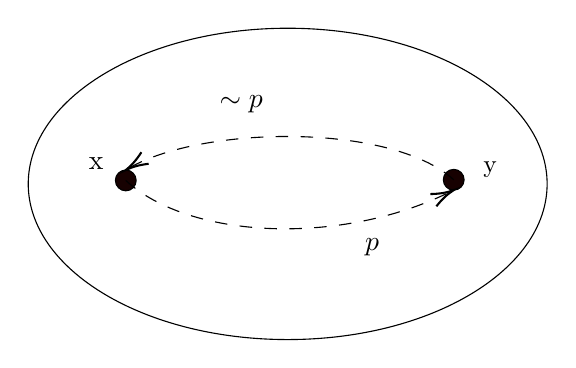
\begin{tikzpicture}[x=0.75pt,y=0.75pt,yscale=-1,xscale=1]
%uncomment if require: \path (0,300); %set diagram left start at 0, and has height of 300

%Shape: Ellipse [id:dp7216176657267284]
\draw   (220,155) .. controls (220,113.58) and (275.96,80) .. (345,80) .. controls (414.04,80) and (470,113.58) .. (470,155) .. controls (470,196.42) and (414.04,230) .. (345,230) .. controls (275.96,230) and (220,196.42) .. (220,155) -- cycle ;
%Shape: Circle [id:dp028557385614719877]
\draw  [fill={rgb, 255:red, 23; green, 1; blue, 1 }  ,fill opacity=1 ] (262,153.33) .. controls (262,150.56) and (264.24,148.33) .. (267,148.33) .. controls (269.76,148.33) and (272,150.56) .. (272,153.33) .. controls (272,156.09) and (269.76,158.33) .. (267,158.33) .. controls (264.24,158.33) and (262,156.09) .. (262,153.33) -- cycle ;
%Shape: Circle [id:dp44344880871890213]
\draw  [fill={rgb, 255:red, 23; green, 1; blue, 1 }  ,fill opacity=1 ] (420,153) .. controls (420,150.24) and (422.24,148) .. (425,148) .. controls (427.76,148) and (430,150.24) .. (430,153) .. controls (430,155.76) and (427.76,158) .. (425,158) .. controls (422.24,158) and (420,155.76) .. (420,153) -- cycle ;
%Curve Lines [id:da7287709889449594]
\draw  [dash pattern={on 4.5pt off 4.5pt}]  (267,153.33) .. controls (297.69,181.71) and (370.52,184.94) .. (423.4,158.8) ;
\draw [shift={(425,158)}, rotate = 153.7] [color={rgb, 255:red, 0; green, 0; blue, 0 }  ][line width=0.75]    (10.93,-3.29) .. controls (6.95,-1.4) and (3.31,-0.3) .. (0,0) .. controls (3.31,0.3) and (6.95,1.4) .. (10.93,3.29)   ;
%Curve Lines [id:da6566329581802051]
\draw  [dash pattern={on 4.5pt off 4.5pt}]  (425,153) .. controls (394.47,125.42) and (303.78,126.95) .. (268.57,147.38) ;
\draw [shift={(267,148.33)}, rotate = 327.9] [color={rgb, 255:red, 0; green, 0; blue, 0 }  ][line width=0.75]    (10.93,-3.29) .. controls (6.95,-1.4) and (3.31,-0.3) .. (0,0) .. controls (3.31,0.3) and (6.95,1.4) .. (10.93,3.29)   ;

% Text Node
\draw (438,143) node [anchor=north west][inner sep=0.75pt]  [font=\small] [align=left] {y};
% Text Node
\draw (381,180) node [anchor=north west][inner sep=0.75pt]   [align=left] {$\id{p}$};
% Text Node
\draw (248,141) node [anchor=north west][inner sep=0.75pt]   [align=left] {x};
% Text Node
\draw (311,111) node [anchor=north west][inner sep=0.75pt]   [align=left] {$\sim \id{p}$};

\end{tikzpicture}

\caption{A path from x to y along with its inversion, i.e.\ the commutativity of equality}
\end{figure}

Compared to the version of \id{Eq\_comm} presented in
\autoref{sec:typer-old-eq}, this version is more intuitive and more aptly
captures the idea of `inverting' an equality proof.

\subsubsection*{Functional extensionality}\label{subsec:funext}
The notion of functional extensionality implies that pointwise-equal functions
are indeed equal. This often makes an appearance in mathematical proofs, it will
especially be required to prove the effectiveness of quotients in
\autoref{ch:quotient-effectiveness}. However, as we shall see in
\autoref{sec:quot-implies-funext}, the existence of quotient types itself is
sufficient to derive functional extensionality. Although functional
extensionality is a property that is respected by all functions, in most proof
assistants, it is not provided nor is it derivable. If one requires it, it would
then have to be postulated as an axiom, therefore adversely affecting the
computational behaviour of a system as we would describe below. By postulating
%% Note: IIRC it suffices to define the interval type as a HIT for funext to be
%% derivable, is this worth mentioning? Maybe... maybe not...
the existence of the interval type along with an equality type that's
based on it, functional extensionality can be derived as a theorem as we
illustrate below.

\begin{minted}[escapeinside=||,mathescape=true]{agda}
    Eq_funExt : (f g : (?A |$\rightarrow$| ?B)) |$\Rightarrow$| (p : (x : ?A) |$\rightarrow$| f x |$\equiv$| g x) |$\rightarrow$| f |$\equiv$| g
    Eq_funExt p = Eq_eq (f := |$\lambda$| i |$\Rrightarrow$| |$\lambda$| x |$\rightarrow$| Eq_uneq (p := p x) (i := i))
\end{minted}

We note that the above proof makes use of the $\eta$-equivalence of functions,
i.e. $(\lambda \id{x} \rightarrow \Funapp{\id{f}}{\id{x}}) = \id{f}$.

%% NOTE: Skipping this because I would already have mentioned it while
%% introducing Cubical Agda in an earlier chapter

%% Another
%% %% SM: Funny, I tend to think of it the other way around, i.e. that
%% %% Eq_uneq lets us treat the equality type as a function from I.
%% thing that is worth noting is that we interpret erasable functions out of $\bI$
%% themselves as an equality type, i.e.\ if we do without the $\id{Eq\_eq}$
%% constructor, and if we think of $\id{Eq\_uneq}$ as the direct application of an
%% argument of type $\bI$ to such a function, we obtain the following
%% interpretation of $\id{Eq\_funExt}$ as is the case in Cubical Agda.

%% %% SM: You can't presume the readers are familiar with Cubical Agda and
%% %% its syntax.  So you need to hand-hold them through the code.
%% %% Maybe you can avoid some of it by showing it using a Typer-style syntax
%% %% and explaining the changes that would need to be taken from Cubical Agda
%% %% to make it work.
%% %% SM: IOW always keep in mind that the PL world loves to introduce
%% %% new notations but that makes our work impenetrable to outsiders.
%% %% So try and use as few different notations as possible.
%% \begin{minted}[escapeinside=||,mathescape=true]{agda}
%% funExt : |$\forall$| {A B : Type |$\ell$|} {f g: A |$\rightarrow$| B}
%%          |$\rightarrow$| (p : (x : A) |$\rightarrow$| f x |$\equiv$| g x)
%%          |$\rightarrow$| f |$\equiv$| g
%% funExt p i x = p x i
%% \end{minted}

%% The proof $\id{p}$ that the functions are extensionally equal may be seen to
%% have the type $\id{A} \rightarrow \bI \rightarrow B$, on other hand, a proof
%% that the functions are equal would have the type $\bI \rightarrow (A \rightarrow
%% B)$. In this case, it becomes clear that a proof of functional extensionality
%% merely needs to swap the order of its two arguments. This is observed in several
%% recent proof assistants that implement cubical type theory, such as Cubical Agda
%% as mentioned before, as well as coolTT and redTT.\@

\subsubsection*{Congruence of equality}\label{subsec:congruence-eq}
This is another typical property of equality whose proof is significantly
simplified in a system with a cubical equality.

%% Eq_cong : (x : ?A) => (y : ?A) =>
%%           (f : ?A -> ?) -> (p : Eq x y)
%%           -> Eq (f x) (f y)
%% Eq_cong = lambda f -> lambda p ->
%%             Eq_eq (f := lambda i ≡> f (Eq_uneq (p := p) (i := i)))
\begin{minted}[escapeinside=||,mathescape=true]{agda}
    Eq_cong : (x y : ?A) |$\Rightarrow$| (g : (?A |$\rightarrow$| ?B)) |$\rightarrow$| (p : x |$\equiv$| y) |$\rightarrow$| g x |$\equiv$| g y
    Eq_cong g p = Eq_eq (f := |$\lambda$| i |$\Rrightarrow$| g (Eq_uneq (p := p) (i := i)))
\end{minted}

To construct a proof of \fn{g x $\equiv$ g y}, we apply the \id{Eq\_eq}
constructor to a function that returns \fn{g x} when called with $\ileft$ and
\fn{g y} when called with $\iright$. We construct this function by
deconstructing the proof \id{p} using \id{Eq\_uneq} followed by applying it to
the function \id{g}. Conceptually speaking we are simply placing a call to
\id{g} `inside' the equality proof \id{p}. By the $\eta$-equivalence of the
equality type described in \autoref{sec:identity}, we also have that
$\fn{Eq\_cong id p = p}$ holds definitionally\footnote{\id{id} is the
polymorphic identity function}.

%% TODO: Let's skip this too since I skipped a similar thing in the prev section

%% Like before, we examine the definition of the theorem in Cubical Agda for a
%% change of perspective. We observe that the congruence of equality merely
%% involves applying the function $\id{f}$ to the terms at both endpoints of the
%% equality.

%% \begin{minted}[escapeinside=||,mathescape=true]{agda}
%% congS : |$\forall$| {A B : Type |$\ell$|} |$\rightarrow$| (f : A |$\rightarrow$|
%% B) (p : x |$\equiv$| y) |$\rightarrow$| f x |$\equiv$| f y congS f p i = f (p i)
%% \end{minted}

%% TODO: Figure this out
%%
%% \subsection{Limitations}
%% We don't have primitives such as $hcomp$, what does this imply? Is there a
%% certain class of proofs we are unable to construct? Or do we just suffer from
%% some amount of inconvenience?

%% From what I understand, this allows us to compose higher dimensional cubes, i.e.
%% we don't really need or care about this here I believe. So either don't mention it,
%% or briefly touch on it at the very end.

\section{Quotient Types}\label{sec:quot}

In this section, we introduce our implementation of quotient types in Typer. We
opted for an implementation more or less in accordance with the rules presented
by Hoffman\cite[Chap~5.1.5]{hofmann1995extensional}. This may be seen as a
compromise as our quotient types do not benefit from the convenience that one
gets with HITs and QITs that allow the definition of arbitrary equation
constructors. Our minimalistic approach provides an implementation of quotient
types that is sufficient for general programming without requiring an extensive
overhaul of the existing system. In the rest of this section, we give an
abstract presentation of the syntax of the new constructs followed by their
typing and computation rules. We then show how the above is adapted to Typer
code.

\subsection{Syntax}\label{sec:quot-syntax}

We give an abstract presentation of the syntax of the new constructs that we
introduce in this section:

\setlength{\grammarparsep}{20pt plus 1pt minus 1pt} % increase separation between rules
\setlength{\grammarindent}{4em} % increase separation between LHS/RHS

%% SM: BTW, I completely forgot about it, but the convention we usually
%% use in Type is to use capitalized names for types, non-capitalized
%% names for constants and functions, and to use the same name for a type
%% and for its constructor (modulo capitalization) if there's only one
%% constructor.  So `Quotient_in` could be `quotient`.

%% The `renewcommands` make the angle brackets go away
\renewcommand{\syntleft}{}
\renewcommand{\syntright}{}
\begin{grammar}
<$T$> ::= \ldots
\alt{} \fn{Quotient $T_{A}$ $T_{R}$}
\alt{} \fn{Quotient_in $T_{R}$ $T_{a}$}
\alt{} \fn{Quotient_eq $T_{r}$}
\alt{} \fn{Quotient_elim $T_{f}$ $T_{p}$ $T_{q}$}
\alt{} \fn{Quotient_trunc $T_{p}$ $T_{q}$}
\end{grammar}

We added a new \id{Quotient} type former, we can construct a quotient type using
the \fn{Quotient A R} syntax. Here, \id{A} is the base type of the quotient and
\id{R} is a binary relation defined on \id{A}. In order to project a term \id{a}
into the quotient \fn{Quotient A R}, we use the syntax \fn{Quotient\_in R a}.
The projection requires us to specify what the underlying relation of the
quotient should be. Given that we have some evidence \id{r} that two terms
\id{a$_1$} and \id{a$_2$} are related by some quotient, we can construct an
equality proof that says that their projections into a quotient based on the
aforementioned relation are equal using the \fn{Quotient\_eq r} syntax. For two
terms \id{p} and \id{q} that are both equality proofs between quotient terms,
\id{Quotient\_trunc p q} constructs a proof that the proof terms themselves are
equal, `trunc' here refers to the set \underline{trunc}ation of quotients. The
relevance of this is not immediately clear, we defer an explanation of this to
section \autoref{sec:rec2}, readers are encouraged to trust that this is a
necessary addition for now. Finally, the elimination of a term \id{q} of a
quotient type is done using the syntax \fn{Quotient\_elim f h q} where \id{f} is
a function out of the base type and \id{h} is proof that \id{f} is compatible
with the underlying relation of the quotient.

For instance, we could define the integers as a quotient \fn{Z = Quotient (Nat
  $\times$ Nat) R$_Z$}\footnote{The \fn{_$\times$_} syntax that we use is a
shorthand for the $\Sigma$ type when the second projection does not depend on
the first.} with \fn{R$_Z$ = $\lambda$ <a , b> <c , d> $\rightarrow$ a + d
  $\equiv$ c + b} . For instance, we can construct the integer 0 using the
syntax \fn{Quotient\_in R$_Z$ <0 , 0>}. We can also construct a proof that the
pair \fn{<1 , 1>} would also correspond to the integer 0 by using the fact that
natural number addition is commutative like so: \fn{Quotient\_eq (Nat+\_comm 0
  1) :\@ Quotient\_in R$_Z$ <0 , 0> $\equiv$ Quotient\_in R$_Z$ <1 , 1>}. Finally,
we may want to eliminate an integer \id{z} by negating it, for brevity, we omit
the full coherence proof term \id{p}, yielding the following term:
\fn{Quotient\_elim ($\lambda$ <a , b> $\rightarrow$ Quotient\_in R$_Z$ <b , a>)
  p z}.

\subsection{Typing rules}\label{sec:quot-typing-rules}

%% SM: Arguably the "syntax" above is not really new syntax, it's just new
%% primitives, and the typing rules below are renderings of actual types.
%% Maybe you could combine the two in a presentation of the 4 new primitives
%% using their "signature", which I think would be more helpful than
%% the BNF-style which just shows bland "T T T".  E.g.:

%%   Quotient (A : Type) (R : A -> A -> Type) : Type;
%%   Quotient_in (a : ?A) : Quotient ?A ?R;
%%   Quotient_eq (r : R ?a1 ?a2) : Eq (Quotient_in ?a1) (Quotient_in ?a2);
%%   Quotient_elim (f : ?A -> ?B)
%%                 (h : ∀a1,a2.?R a1 a2 -> Eq (f a1) (f a2))
%%                 (q : Quotient ?A ?R)
%%                 : ?B;

%% SM: It's not 100% indispensable that your presentation matches the actual
%% code, as long as the difference is there only to make the material easier
%% to understand.

Now, we present the typing rules of the primitives introduced above. Readers
who are unfamiliar with natural deduction may consult
\autoref{app:natural-deduction} for a short introduction.

\begin{prooftree*}
   \hypo{\oftype{\ctx}{\id{A}}{\kw{Type}}}
   \hypo{\oftype{\ctx}{\id{R}}{\id{A} \rightarrow \id{A} \rightarrow \kw{Type}}}
   \infer2[\textsc{Quot-Formation}]{\oftype{\ctx}{\Funapp{\id{Quotient}}{\id{A}}{\id{R}}}
                                             {\kw{Type}}}
\end{prooftree*}

The $\id{Quotient}$ type former is a function which takes a base type $\id{A}$
along with a relation $\id{R}$ as arguments. At this stage, just like
in\cite{hofmann1995simple}, we do not require the relation to be an equivalence
relation, however, our experience tells us that the above requirement is often
necessary to define a meaningful quotient type.

\begin{prooftree*}
   \hypo{\oftype{\ctx}{\id{a}}{\id{A}}}
   \hypo{\oftype{\ctx}{\Funapp{\id{Quotient}}{\id{A}}{\id{R}}}
                      {\kw{Type}}}
   \infer2[\textsc{Quot-Intro-In}]{\oftype{\ctx}{\Funapp{\id{Quotient\_in}}{\id{R}}{\id{a}}}
   %% \infer2[\textsc{Quot-Intro-In}]{\oftype{\ctx}{\Funapp{\id{Quotient\_in}}{\id{A}}{\id{R}}{\id{a}}}
                                         {\Funapp{\id{Quotient}}{\id{A}}{\id{R}}}}
\end{prooftree*}

$\id{Quotient\_in}$ takes a term \id{a} of type \id{A} and projects it into a
quotient of type \fn{Quotient A R} defined on some relation \id{R}.

\begin{prooftree*}
   \hypo{\oftype{\ctx}{\id{a}_1}{\id{A}}}
   \hypo{\oftype{\ctx}{\id{a}_2}{\id{A}}}
   \hypo{\oftype{\ctx}{\id{r}}{\Funapp{\id{R}}{\id{a}_1}}{\id{a}_2}}
   \infer3[\textsc{Quot-Intro-Eq}]{
\oftype{\ctx}{\Funapp{\id{Quotient\_eq}}{\id{r}}}
             {\Funapp{\id{Quotient\_in}}{\id{R}}{\id{a}_1} \equiv{} \Funapp{\id{Quotient\_in}}{\id{R}}{\id{a}_2}}}
\end{prooftree*}\label{quot-intro-eq-rule}

By definition, given that two terms $\id{a}_1$ and $\id{a}_2$ of type $\id{A}$
are related by some relation \id{R}, then the projections of these two terms
into a quotient under the relation \id{R} should be equal. $\id{Quotient\_eq}$
is a witness of the above property.

\begin{prooftree*}
   \hypo{\oftype{\ctx}{\id{a}_1}{\fn{Quotient A R}}}
   \hypo{\oftype{\ctx}{\id{a}_2}{\fn{Quotient A R}}}
   \infer[no rule]2{\oftype{\ctx}{p}{\id{a}_1 \equiv{} \id{a}_2} \ \ \ \oftype{\ctx}{q}{\id{a}_1 \equiv{} \id{a}_2}}
   \infer1[\textsc{Quot-Intro-Trunc}]{
\oftype{\ctx}{\Funapp{\id{Quotient\_trunc}}{\id{p}}{\id{q}}}
             {\id{p} \equiv{} \id{q}}}
\end{prooftree*}\label{quot-intro-trunc-rule}

\id{Quotient\_trunc} is a witness of the uniqueness of equality proofs between
quotient terms. For any two terms \id{p} and \id{q} that are equality proofs
between two quotient terms, \id{Quotient\_trunc} constructs a proof of equality
between \id{p} and \id{q}.

\begin{prooftree*}
   \hypo{\oftype{\ctx}{\id{P}}{\Funapp{\id{Quotient}}{\id{A}}{\id{R}} \rightarrow \kw{Type}}}
   \hypo{\oftype{\ctx}{\id{q}}{\Funapp{\id{Quotient}}{\id{A}}{\id{R}}}}
   \infer[no rule]2{\oftype{\ctx}{\id{f}}
                           {(\oftype{\id{a}}{\id{A}}) \rightarrow \Funapp{\id{P}}{(\Funapp{\id{Quotient\_in}}{\id{R}}{\id{a}})}}}
   \infer[no rule]1{\oftype{\ctx}{\id{h}}{(\oftype{\id{a}_1 \ \id{a}_2}{\id{A}})
                                          \rightarrow \Funapp{\id{R}}{\id{a}_1}{\id{a}_2}}
                                          \rightarrow \Funapp{\id{Heq}}{(\Funapp{\id{f}}{\id{a}_1})}
                                                                       {(\Funapp{\id{f}}{\id{a}_2})}}
   \infer1[\textsc{Quot-Elim}]{\oftype{\ctx}{\Funapp{\id{Quotient\_elim}}{\id{f}}{\id{h}}{\id{q}}}
                                        {\Funapp{\id{P}}{\id{q}}}}
\end{prooftree*}

We would like to enable the dependent elimination of quotients, in other words,
we want to eliminate a term of some quotient type
$\Funapp{\id{Quotient}}{\id{A}}{\id{R}}$ to some type family $\id{P}$ that is
indexed by the quotient type itself. So far, our implementation has been rather
similar to \Lean{}'s (see \autoref{sec:intro-lean-quotients}). However, unlike
\Lean{}'s \id{Quot.ind}, the elimination motive $\id{P}$ does not have to be a
proposition, giving us more flexibility. To construct an example of this, we
first introduce a new definition. A type is said to be \emph{decidable} if we
can decide whether the type is inhabited or not. In the case where it is
inhabited, we must have a witness of such an inhabitant. In Typer, decidability
can be represented by the following inductive type by using the `propositions
as types' variation of logical negation, \id{Not}, as introduced in
\autoref{subsec:log-neg}.

\begin{minted}[escapeinside=@@,mathescape=true]{agda}
    type Dec (A : Type)
      | yes A
      | no (Not A)
\end{minted}

For this example, we reuse the definition of integers given in
\autoref{sec:quot-syntax}. We might want to define a function that
\emph{decides} whether a certain integer is positive, i.e.\ of type \fn{(z
  :\@ Z) $\rightarrow$ Dec (isPos z)}. This is known as dependent
elimination as the term that we are trying to eliminate, \id{z}, is itself
present in the return type. To perform the elimination of a quotient, we require
some function $\id{f}$ that takes some $\id{a}$ of the base type $\id{A}$ to
$\Funapp{\id{P}}{(\Funapp{\id{Quotient\_in}}{\id{A}}{\id{R}}{\id{a}})}$. In a
way, this implies that the function $\id{f}$ has the chance of `looking inside'
the quotient, and thus we also require a proof that such a function $\id{f}$
behaves consistently when applied to terms that are related by the underlying
relation of the quotient. The usage of heterogeneous equality here is necessary
as $\Funapp{\id{f}}{\id{a}_1}$ and $\Funapp{\id{f}}{\id{a}_2}$ are not
necessarily of the \textbf{same} type.

\subsection{Reduction rules}\label{quot-red-rules}
We present the computation rule for the elimination of quotients.

\begin{prooftree*}
   \infer0{\id{Quotient\_elim} \ \ \id{f} \ \ \id{p}
     \ \ (\id{Quotient\_in} \ \ \id{R} \ \ \id{a}) \leadsto
     \Funapp{\id{f}}{\id{a}}}
\end{prooftree*}

We note that during \id{Quotient} elimination, the proof that the eliminator
function respects the \id{Quotient} is ignored. Instead, the function is applied
directly to the underlying element of the base type. The fact that the proof
that the elimination respects the quotient is unused during computation and is
merely utilised during type-checking justifies our subsequent choice of making
the proof an erasable argument of \id{Quotient\_elim}.

We opted not to provide $\eta$-rules for quotient types as it was unclear to us
which ones would actually be useful. One instance of it that we could possibly
define is the following:

\begin{align*}
  & \id{Quotient\_in} \ \ (\Funapp{\fn{Quotient\_elim}}{\id{f}}{\id{h}}{\id{q}}) \leadsto{} \id{q} \\
\end{align*}

This requires the condition that \id{f} be some function of type \fn{A
  $\rightarrow$ A} such that $\forall \id{a} \ . \ \fn{R a (f a)}$ is valid. For
instance, such a condition would, for instance, be fulfilled if \id{f} was a
normalisation function on \id{A}. However, the above requirement is not easily
enforced, not to mention that the $\eta$-rule itself is not necessarily that
useful to have. Another similar $\eta$-rule that is more easily enforced is the
following:

\begin{align*}
  & \fn{Quotient\_elim} \ \  \id{Quotient\_in} \ \ (\lambda \ \id{a} \ \id{a'} \ \id{r} \rightarrow \Funapp{\id{Quotient\_eq}}{\id{r}}) \ \id{q} \leadsto{} \id{q} \\
\end{align*}

This rule says that if the elimination of a quotiented term \id{q} simply
applies the projection into the quotient under the same relation, then the
entire elimination may be seen as a no-op on \id{q}. Such a rule makes a great
deal of sense, however we believe that it is of limited practical utility. We
show, however, that these $\eta$-equivalences may be proven propositionally in
\autoref{app:quotient-eta} of the appendix.

\subsection{Implementation}

In this section, we describe how the rules described above were added to Typer.
Subsequently, we describe some syntactic sugar that facilitates the usage of
quotient types.

\subsubsection{Primitives}

The quotient constructs presented in the previous sections are implemented in
Typer as primitives. In this subsection, we present their types and justify our
choices where appropriate. For brevity, we do not explicitly indicate that the
below functions are universe polymorphic.

\paragraph{Formation}
The $\id{Quotient}$ type former has the following type:

\begin{minted}[escapeinside=||,mathescape=true]{agda}
    Quotient : (A : Type) |$\rightarrow$| (R : A |$\rightarrow$| A |$\rightarrow$| Type) |$\rightarrow$| Type
\end{minted}

\paragraph{Introduction}
Two primitives are added, corresponding to the two introduction rules of $\id{Quotient}$.

\begin{minted}[escapeinside=||,mathescape=true]{agda}
Quotient_in : ?A |$\rightarrow$| Quotient ?A ?R
Quotient_eq : ?R ?a ?a' |$\rightarrow$| Quotient_in (R := ?R) ?a |$\equiv$| Quotient_in (R := ?R) ?a'
\end{minted}

The \id{Quotient\_in} primitive may be seen as a box that stores an expression
of the base type \id{A}. Such a value may only be accessed by a subsequent usage
of the eliminator, which we describe shortly. Arguments \id{A} and \id{R} are
made implicit as they can often be inferred from the context.

We postulated \id{Quotient\_eq} as an axiom to witness the equality between the
projections of two related terms.

\paragraph{Elimination}

\begin{minted}[escapeinside=||,mathescape=true]{agda}
Quotient_elim : (P : Quotient ?A ?R |$\rightarrow$| Type)
                |$\Rrightarrow$| (f : (a : ?A) |$\rightarrow$| P (Quotient_in a))
                |$\rightarrow$| ((a a' : ?A) |$\rightarrow$| ?R a a' |$\rightarrow$| Heq (f a) (f a'))
                |$\Rrightarrow$| (q : Quotient ?A ?R) |$\rightarrow$| P q
\end{minted}

The \id{Quotient\_elim} is implemented as a primitive with the appropriate
$\beta$-reduction rule mentioned in the previous section. When
$\id{Quotient\_elim}$ is passed a term of the form
$\Funapp{\id{Quotient\_in}}{\id{a}}$, the entire $\id{Quotient\_elim}$ term
reduces to just $\Funapp{\id{f}}{\id{a}}$, ignoring the coherence proof that is
passed to the function as it acts simply as a form of static information. Since
the proof itself is computationally irrelevant, it is made to be an erasable
argument.


The non-dependent eliminator, \id{Quotient\_rec}, is merely a special case of
\id{Quotient\_elim} where \id{P} is a constant type family. Hence, we define
\id{Quotient\_rec} in terms of \id{Quotient\_elim} as follows:

\begin{minted}[escapeinside=||,mathescape=true]{agda}
Quotient_rec : (f : ?A |$\rightarrow$| ?B)
               |$\rightarrow$| (p : (a a' : ?A) |$\rightarrow$| ?R a a' |$\rightarrow$| f a |$\equiv$| f a')
               |$\Rrightarrow$| Quotient ?A ?R |$\rightarrow$| ?B
Quotient_rec f q = Quotient_elim (R := R) (P := |$\lambda$| _ |$\rightarrow$| B) f (p := p) q
\end{minted}

\subsection{Syntactic sugar}

\paragraph{qcase}

We provide some syntactic sugar to simplify the non-dependent elimination
quotients. The syntax we opted for is reminiscent of that of
Arend's\cite{arend}. The elimination of a quotient expression is done in the
style of a case analysis where both the term and path constructors have to be
addressed with the following syntax:

\begin{minted}[escapeinside=@@,mathescape=true]{agda}
    qcase q
      | Quotient_in a @$\Rightarrow$@ e1
      | Quotient_eq x y r @$\Rightarrow$@ e2
\end{minted}

\id{q} is the scrutinee of the case analysis. A type annotation may be given to it
by specifying the base type and relation of the quotient, e.g. \fn{(e :\@ A / R)}.
The variable \id{a} is defined in the scope of \id{e1} and the variables \id{x},
\id{y}, and \id{r} are defined in the scope of \id{e2}. The bound variables are
the parameters of the two constructors of \id{Quotient}. In the first branch, we
say what we would like to map a quotient expression to. In the second branch, we
prove that the above mapping respects the quotient by constructing a term
\fn{e2 :\@ [x/a]e1 $\equiv$ [y/a]e2}.

To illustrate how this works, we construct a simple example based on the
quotient of the \id{A $\rightarrow$ B} type along with a relation
\id{PointwiseEq} that represents the pointwise equality of such functions. We
then define a function that composes quotiented functions with plain functions
of type \id{B $\rightarrow$ C} to produce functions of type \id{A $\rightarrow$
  C}.

%% SM: Using the Unit type makes it a bit too trivial, I think.
%% How 'bout using the Boolean type with:
%%     R a1 a2  = Unit    %% (not sure which of Unit or True is better here)
%% and have an elimination like:
%%     Quotient_in a => if a then 1 else 1
%%     Quotient_eq a a' r => Quotient_eq (not a) (not a') unit
%% \begin{minted}[escapeinside=@@,mathescape=true]{agda}
%% R : Unit @$\rightarrow$@ Unit @$\rightarrow$@ Type
%% R u1 u2 = Unit

%% e1 : Quotient Unit R @$\rightarrow$@ Unit
%% e1 q = qcase (q : Unit / R)
%%         | Quotient_in a @$\Rightarrow$@ ()
%%         | Quotient_eq a a' r @$\Rightarrow$@ Eq_refl
%% \end{minted}

\begin{minted}[escapeinside=@@,mathescape=true]{agda}
    PointwiseEq : (A : ?) @$\Rightarrow$@ (B : ?) @$\Rightarrow$@ (A @$\rightarrow$@ B) @$\rightarrow$@ (A @$\rightarrow$@ B) @$\rightarrow$@ Type
    PointwiseEq f g = (x : A) @$\rightarrow$@ f x @$\equiv$@ g x

    e1 : Quotient (?A @$\rightarrow$@ ?B) PointwiseEq @$\rightarrow$@ (?B @$\rightarrow$@ ?C) @$\rightarrow$@ ?A @$\rightarrow$@ ?C
    e1 q g a = qcase (q : (A @$\rightarrow$@ B) / PointwiseEq)
            | Quotient_in f @$\Rightarrow$@ g (f a)
            | Quotient_eq f f' r @$\Rightarrow$@ Eq_cong g (r a)
\end{minted}

Drawing inspiration from Arend, the \id{Quotient\_eq} branch may also be handled
by introducing an Interval variable into the scope. Instead of directly
constructing an equality proof, we simply specify what the given map for the
\id{Quotient\_in} branch would map us to for a certain endpoint \id{i} of the
\id{Quotient\_eq} proof. We may rewrite the above example as follows:

%% SM: Hmm... indeed my Boolean example doesn't work well here,
%% unless we changed Quotient_eq to return a function `I ≡> Quotient A R`
%% rather than an equality. 🙁
%% It would be good to find n example that's similarly simple as the
%% one I suggest above but which can also benefit from this "path notation",
%% \begin{minted}[escapeinside=@@,mathescape=true]{agda}
%% e2 : Quotient Unit R @$\rightarrow$@ Unit
%% e2 q = qcase (q : Unit / R)
%%         | Quotient_in a @$\Rightarrow$@ ()
%%         | Quotient_eq a a' r i @$\Rightarrow$@ ()
%% \end{minted}

\begin{minted}[escapeinside=@@,mathescape=true]{agda}
    e2 : Quotient (?A @$\rightarrow$@ ?B) PointwiseEq @$\rightarrow$@ (?B @$\rightarrow$@ ?C) @$\rightarrow$@ ?A @$\rightarrow$@ ?C
    e2 q g a = qcase (q : (A @$\rightarrow$@ B) / PointwiseEq)
            | Quotient_in f @$\Rightarrow$@ g (f a)
            | Quotient_eq f f' r i @$\Rightarrow$@ g (Eq_uneq (p := r a) (i := i))
\end{minted}

More examples of usages of this macro are given in subsequent sections.

\chapter{Equality Theorems}\label{ch:eq-theorems}
In addition to the examples given in \autoref{subsec:eq-examples}, we derive
more theorems related to the equality type, some of which shall facilitate the
use of quotient types.

\section{Cast}\label{sec:eq-transport}
As mentioned in \autoref{sec:typer-old-eq}, the cast operation\footnote{This is
also known as the transport operation, as is most often the case in a HoTT
setting.} is an implementation of Leibniz's principle of the indiscernibility of
identicals. Instead of defining it as a primitive as was done in the
aforementioned section, we now define it in terms of the interval primitive,
\id{I\_transp} described in \autoref{sec:i-transp}.

%% Eq_cast : (x : ?) ≡> (y : ?) ≡> (p : Eq x y) ≡> (f : ? -> ?)
%%             ≡> f x -> f y
%% Eq_cast = lambda _ ≡> lambda _ ≡> %% Two level variables
%%            lambda A ≡> %% Type of x and y
%%            lambda x ≡> lambda y ≡>
%%            lambda p ≡> lambda f ≡>
%%              lambda fx ->
%%                 I_transp (A := lambda i ≡> f (Heq_uneq
%%                                               (t := lambda _ ≡> A)
%%                                               (p := p) (i := i)))
%%                          (r := i0) fx
%%

\begin{minted}[escapeinside=||,mathescape=true]{agda}
    Eq_cast : (x y : ?A) |$\Rrightarrow$| (p : x |$\equiv$| y) |$\Rrightarrow$| (f : ?A |$\rightarrow$| Type) |$\Rrightarrow$| f x |$\rightarrow$| f y
    Eq_cast A x y p f fx =
      I_transp (A := |$\lambda$| t |$\Rrightarrow$| f (Eq_uneq (t := t) (p := p) (i := i)))
               fx (r := |$\iright$|)
\end{minted}

Here, we make use of the built-in function $\id{I\_transp}$ by passing it the
argument $\earg{\id{r}}{\iright}$, intending it to behave as a cast function. In
other words, by passing it something of type $\Funapp{\id{f}}{\id{x}}$, it
returns something of type $\Funapp{\id{f}}{\id{y}}$, which is precisely what the
cast function is meant to do.

\paragraph{Equality Between \id{x} and \kw{cast}$_x$}\label{app:cast-is-eq}

Transporting across a reflexive path should be equivalent to a no-op, as
illustrated in the following proof.

\begin{minted}[escapeinside=||,mathescape=true]{agda}
    Eq_cast_refl : (A : Type) |$\Rrightarrow$| (x : A)
                   |$\rightarrow$| x |$\equiv$| Eq_cast (p := Eq_refl (x := A)) (f := id) x
    Eq_cast_refl A x = Eq_refl
\end{minted}

The above is possible because of the first reduction rule of \id{I\_transp},
allowing us to recover the reduction rule of Typer's existing implementation of
\id{Eq\_cast} as presented in \autoref{sec:typer-old-eq}. With cubical equality,
this property is not restricted to reflexivity, it may be generalised to
arbitrary equality proofs by using the special property of \id{I\_transp}.

\begin{minted}[escapeinside=@@,mathescape=true]{agda}
castIsEq : (A : I @$\Rrightarrow$@ Type) @$\Rrightarrow$@ (x : A (_ := @$\ileft$@))
           @$\rightarrow$@ Heq (t := A) x (Eq_cast (p := Eq_eq (f := A)) (f := id) x)
castIsEq = @$\lambda$@ A @$\Rrightarrow$@ @$\lambda$@ x @$\rightarrow$@
  let
    p : I_transp (A := A) x (r := @$\iright$@) @$\equiv$@ Eq_cast (p := Eq_eq (f := A)) (f := id) x
    p = Eq_eq (f := @$\lambda$@ j @$\Rrightarrow$@
                    I_transp (A := @$\lambda$@ i @$\Rrightarrow$@ Eq_uneq (p := Eq_@$\eta$@ (A := A) i) (i := j))
                             x (r := @$\iright$@))

   h : Heq (t := A) x (I_transp (A := A) x (r := @$\iright$@))
   h = Heq_eq (t := A)
              (f := @$\lambda$@ i @$\Rrightarrow$@ I_transp (A := A) x (r := i))
  in
    Eq_cast (p := p) (f := @$\lambda$@ e @$\rightarrow$@ Heq (t := A) x e) h
\end{minted}


\fn{I_transp (A := A) x (r := $\iright$)} and \fn{Eq_cast (p := Eq_eq (f := A)) (f :=
  id) x} are not definitionally equal since the $\eta$-equivalence \fn{A (_ :=
  i)) $\equiv$ (Eq_uneq (p := Eq_eq (f := A)) (i := i))} does not hold
definitionally. Hence, we prove the $\eta$-equivalence propositionally and use
it to complete our proof.

\begin{minted}[escapeinside=@@,mathescape=true]{agda}
    Eq_@$\eta$@ : (A : I @$\Rrightarrow$@ Type) @$\Rrightarrow$@ (i : I)
           @$\rightarrow$@ A (_ := i) @$\equiv$@ Eq_uneq (p := Eq_eq (f := A)) (i := i)
    Eq_@$\eta$@ = @$\lambda$@ A @$\Rrightarrow$@ @$\lambda$@ i @$\rightarrow$@
      case i return A (_ := i) @$\equiv$@ Eq_uneq (p := Eq_eq (f := A)) (i := i)
        | @$\ileft$@ @$\Rightarrow$@ Eq_refl
        | @$\iright$@ @$\Rightarrow$@ Eq_refl
\end{minted}

%% NOTE: This is just an extra piece of information that may or may not interest
%% readers, i.e. the kind of thing that I could potentially remove

In Typer and in intensional type theory in general, we need to explicitly invoke
a cast function of some sort, this is in contrast with extensional type theory
(ETT)\cite{martin1982constructive} where equality proofs in the context are
automatically used by the type-checker to perform casts whenever necessary. This
is shown by the following judgment in ETT that states that equality proofs can
be converted to judgemental equalities.

\begin{prooftree*}
  \hypo{\oftype{\ctx}{t}{a \equiv b}}
  \infer1{\ctx \vdash a \simeq b}
\end{prooftree*}

This is also the reason why type-checking is not decidable in ETT as the
necessity to invoke the above rule is not syntax-directed.

\section{Transitivity}\label{sec:eqtransitivity}
Continuing our analogy of equality proofs as paths, the transitivity property
allows us to concatenate two paths. We join the right endpoint of the first path
with the left endpoint of the second path to produce a new path, represented by
the dotted line in \autoref{fig:eq-trans}. The proof of this theorem is as
follows:

\begin{minted}[escapeinside=||,mathescape=true]{agda}
    Eq_trans : (x y z : ?t) |$\Rrightarrow$| x |$\equiv$| y |$\rightarrow$| y |$\equiv$| z |$\rightarrow$| x |$\equiv$| z
    Eq_trans x=y y=z = Eq_cast (p := y=z) (f := |$\lambda$| x' |$\rightarrow$| x |$\equiv$| x') x=y
\end{minted}

\begin{figure}
\centering
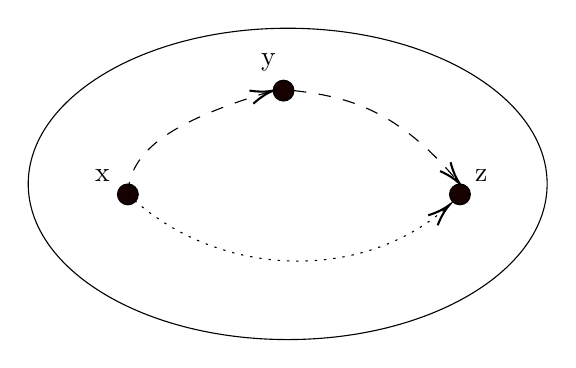
\begin{tikzpicture}[x=0.75pt,y=0.75pt,yscale=-1,xscale=1]
%uncomment if require: \path (0,300); %set diagram left start at 0, and has height of 300

%Shape: Ellipse [id:dp014634117148388581]
\draw   (210,155) .. controls (210,113.58) and (265.96,80) .. (335,80) .. controls (404.04,80) and (460,113.58) .. (460,155) .. controls (460,196.42) and (404.04,230) .. (335,230) .. controls (265.96,230) and (210,196.42) .. (210,155) -- cycle ;
%Shape: Circle [id:dp26323124675512766]
\draw  [fill={rgb, 255:red, 23; green, 1; blue, 1 }  ,fill opacity=1 ] (253,160.06) .. controls (253,157.3) and (255.24,155.06) .. (258,155.06) .. controls (260.76,155.06) and (263,157.3) .. (263,160.06) .. controls (263,162.82) and (260.76,165.06) .. (258,165.06) .. controls (255.24,165.06) and (253,162.82) .. (253,160.06) -- cycle ;
%Shape: Circle [id:dp6819431699402925]
\draw  [fill={rgb, 255:red, 23; green, 1; blue, 1 }  ,fill opacity=1 ] (328,110.06) .. controls (328,107.3) and (330.24,105.06) .. (333,105.06) .. controls (335.76,105.06) and (338,107.3) .. (338,110.06) .. controls (338,112.82) and (335.76,115.06) .. (333,115.06) .. controls (330.24,115.06) and (328,112.82) .. (328,110.06) -- cycle ;
%Curve Lines [id:da09243595336985422]
\draw  [dash pattern={on 4.5pt off 4.5pt}]  (338,110.06) .. controls (364.73,112.97) and (388.52,119.86) .. (417.13,154.01) ;
\draw [shift={(418,155.06)}, rotate = 229.87] [color={rgb, 255:red, 0; green, 0; blue, 0 }  ][line width=0.75]    (10.93,-3.29) .. controls (6.95,-1.4) and (3.31,-0.3) .. (0,0) .. controls (3.31,0.3) and (6.95,1.4) .. (10.93,3.29)   ;
%Curve Lines [id:da576198955407853]
\draw  [dash pattern={on 4.5pt off 4.5pt}]  (258,160.06) .. controls (258.99,139.27) and (277.62,125.28) .. (326.51,110.51) ;
\draw [shift={(328,110.06)}, rotate = 163.36] [color={rgb, 255:red, 0; green, 0; blue, 0 }  ][line width=0.75]    (10.93,-3.29) .. controls (6.95,-1.4) and (3.31,-0.3) .. (0,0) .. controls (3.31,0.3) and (6.95,1.4) .. (10.93,3.29)   ;
%Shape: Circle [id:dp7540304044235371]
\draw  [fill={rgb, 255:red, 23; green, 1; blue, 1 }  ,fill opacity=1 ] (413,160.06) .. controls (413,157.3) and (415.24,155.06) .. (418,155.06) .. controls (420.76,155.06) and (423,157.3) .. (423,160.06) .. controls (423,162.82) and (420.76,165.06) .. (418,165.06) .. controls (415.24,165.06) and (413,162.82) .. (413,160.06) -- cycle ;
%Curve Lines [id:da43079739398707617]
\draw  [dash pattern={on 0.84pt off 2.51pt}]  (258,160.06) .. controls (302.55,202.13) and (372.58,201.57) .. (411.82,166.14) ;
\draw [shift={(413,165.06)}, rotate = 136.9] [color={rgb, 255:red, 0; green, 0; blue, 0 }  ][line width=0.75]    (10.93,-3.29) .. controls (6.95,-1.4) and (3.31,-0.3) .. (0,0) .. controls (3.31,0.3) and (6.95,1.4) .. (10.93,3.29)   ;

% Text Node
\draw (321,91) node [anchor=north west][inner sep=0.75pt]   [align=left] {y};
% Text Node
\draw (241,147.06) node [anchor=north west][inner sep=0.75pt]   [align=left] {x};
% Text Node
\draw (424,147.06) node [anchor=north west][inner sep=0.75pt]   [align=left] {z};

\end{tikzpicture}

\caption{The concatenation of a path between x and y and a path between y and z to produce a new path between x and z.}\label{fig:eq-trans}
\end{figure}


\section{J-rule}\label{subsec:j-rule}
The sole term former of the \id{Eq} only allows the construction of reflexive
equalities. At first sight, this leads us to believe that not much can be done
with the \id{Eq} type. After all, if all we had were proofs of the form \fn{x
  $\equiv$ x}, it would be difficult to imagine achieving anything meaningful
with them. The true magic of the equality type lies in its elimination
principle. Traditionally, the equality type comes with an elimination principle
known as the J-rule. This was first introduced by Per Martin-Löf
in\cite{martin1975intuitionistic}. Consider a type family \id{C} that is
parametrised by two terms \id{x} and \id{y} of some type \id{A} as well as a
proof that they are equal, i.e.\ of type \fn{x $\equiv$ y}. If we have a proof
term \id{p} that witnesses the equality of two arbitrary terms \id{a} and \id{b}
of type \id{A}, and we wish to produce a term of type \fn{C a b p}, then the
J-rule says that it suffices for us to provide a means of producing for all
\fn{x :\@ A} a term of type \fn{C x x (refl x)}. We now state the type of the
J-rule:

\begin{minted}[escapeinside=@@,mathescape=true]{agda}
    J : (C : (x y : ?A) @$\rightarrow$@ x @$\equiv$@ y @$\rightarrow$@ Type)
        @$\Rrightarrow$@ ((x : ?A) @$\rightarrow$@ C x x Eq_refl)
        @$\rightarrow$@ (x y : ?A) @$\rightarrow$@ (p : x @$\equiv$@ y)
        @$\rightarrow$@ C x y p
\end{minted}

This rule essentially says that to know what to do with an equality between an
arbitrary \id{x} and \id{y}, we merely need to know how to handle the case where
we are dealing with a reflexivity proof. Now, given the fact that the
reflexivity constructor is the only constructor of the \id{Eq} type, one would
think that the above elimination principle is well justified. Recall that the
elimination principle of strictly positive types\cite{abbott2005containers} can
usually be derived based on the constructors of the datatype itself. For
instance, consider the below inductive definition of the Peano natural numbers.

\begin{minted}{agda}
    type Nat
        | zero
        | succ Nat
\end{minted}

The corresponding elimination principle then takes on the following logical form:

\begin{minted}[escapeinside=@@,mathescape=true]{agda}
    Nat_elim : (P : Nat @$\rightarrow$@ Type) @$\Rrightarrow$@ P zero @$\rightarrow$@ ((n : Nat) @$\rightarrow$@ P n @$\rightarrow$@ P (succ n))
               @$\rightarrow$@ (n : Nat) @$\rightarrow$@ P n
\end{minted}

First, we need to define what needs to be done if the natural number we are
trying to eliminate is \id{zero}. Next, if the natural number we want to
eliminate is something of the form \fn{succ n}, then we can imagine making a
recursive call to the eliminator to produce a result for \fn{succ n} for \id{n},
and now we need a means of transforming a proof of \fn{P n} to one of \fn{P
  (succ n)}. Indeed, the elimination principle of natural numbers is just
mathematical induction. Hence, it is reasonable to say that to eliminate an
equality proof, it suffices for us to define what needs to be done for
reflexivity proofs.

In Typer, the elimination rule for the \id{Eq} type was not provided in the form
of the J-rule before this work, instead, a cast function was provided as
mentioned in a previous section. It is possible to derive \id{Eq\_cast} from the
J-rule. The natural question that we should now ask ourselves is whether the
J-rule can be derived from \id{Eq\_cast}, in other words, we would like to know
if the two elimination principles are equivalent. It turns out that one way of
doing it hinges upon whether we can inhabit the following type:

\begin{minted}[escapeinside=@@,mathescape=true]{agda}
eqUnique : (a b : ?A) @$\rightarrow$@ (p : a @$\equiv$@ b) @$\rightarrow$@ Eq (t := @$\Sigma_{a':A}. a \equiv a'$@) <a, Eq_refl>  <b, p>
\end{minted}

This can be seen as a justification of the J-rule, by fixing one endpoint of an
equality proof to be $\fn{a}$, it is provable that any equality proof between
$\fn{a}$ and some other arbitrary $\fn{b}$ may be proved to be equal to the
reflexivity proof at $\fn{a}$. The exact details of the construction of the
above are given in Appendix~\ref{sec:interval-connections}. Once we have that,
we may easily define the J-rule by performing a cast from \fn{P a Eq\_refl} to
\fn{P b p}:

\begin{minted}[escapeinside=@@,mathescape=true]{agda}
    J h x y p = Eq_cast (p := eqUnique p) (f := @$\lambda$@ <b, p> @$\rightarrow$@ C x b p) (h x)
\end{minted}

\section{Hedberg's theorem}\label{subsec:hedberg}

Although we say that our equality type is a proposition, it is by no means
necessarily a mere proposition (HoTT book\cite[Chap~3.3]{HoTTbook}). This
implies that it is not a given that two proofs of the same equality are
provably equal\cite{hofmann1998groupoid}. In other words, when we ask ourselves
the question ``Is it the case that a = b'', we do not only care if the answer
is yes or no, if they are indeed equal, we could interest ourselves in what
ways exactly are they equal. This is in contrast to other systems where the
Uniqueness of Identity Proofs principle (UIP) applies to all types. Notably,
this is true of systems that admit axiom K\cite{streicher1993investigations}
that states that all equality proofs are equal to the reflexivity proof, and by
extension all proofs of the same equality are equal. An example of a system
%% SM: Does it admit UIP?  I thought it provided it via (yet) an(other) axiom.
%% Oh, I guess it's because it's a Prop, so it's also new in Lean 4.
that admits UIP is \id{Lean}. In the remainder of this section, we show that
UIP is a property that is true for a certain class of types in Typer.

To set the stage, we provide a few definitions. A type is said to be
\emph{decidable} if we can decide whether the type is inhabited or not, this was
presented in more detail in \autoref{sec:quot-typing-rules}. A type is said to
be \emph{collapsed} if any two inhabitants of the type may be proved to be
equal, this corresponds directly to the notion of a mere proposition. The two
definitions that we just stated may also be used in the context of equality
types. If we say that a type has decidable equality, this implies that for any
two terms of this type, we can decide whether or not they are equal. On top of
that, if the type has collapsed equality types, then for any pair of terms of
this type, any two proofs that they are equal are also equal. The notion of
collapsible equality types corresponds to the notion of a \textbf{Set} or
homotopy 0-type in HoTT\cite[Chap~3.1]{HoTTbook}. We represent this using the
following proposition.

\begin{minted}[escapeinside=@@,mathescape=true]{agda}
    isSet : Type @$\rightarrow$@ Type
    isSet A = (x y : A) @$\rightarrow$@ (p q : x @$\equiv$@ y) @$\rightarrow$@ p @$\equiv$@ q
\end{minted}

We shall see in a subsequent section that this property plays a substantial role
in the elimination of quotients in \autoref{sec:rec2}.

\begin{theo}[Hedberg's theorem\cite{hedberg1998coherence}]
If a type \fn{A} has decidable equality, then \fn{A} has collapsed equality
types.
\end{theo}

In this work, we provide a proof of this theorem in the form of Typer code. We
present the type of the function without going into the details of its
implementation\footnote{The actual implementation may be found in the
\href{https://gitlab.com/jamestjw/typer/-/blob/quot-types-v1.0.0/samples/hedberg.typer}{\id{samples/hedberg.typer}}
file}.

\begin{minted}[escapeinside=@@,mathescape=true]{agda}
    dici : (di : (x y : ?A) @$\rightarrow$@ Dec (x @$\equiv$@ y)) @$\rightarrow$@ (a b : ?A) @$\rightarrow$@ (u v : a @$\equiv$@ b)
           @$\rightarrow$@ u @$\equiv$@ v
\end{minted}

The equality of quotient types is not decidable in general, implying that we
cannot use Hedberg's theorem to prove that quotients are Sets. For instance, we
know that the integer type should have decidable equality, however, if we
construct integers by quotienting pairs of natural numbers, we are unable to
prove that the resulting quotient type has decidable equality. This is the
reason why it was necessary to add the \id{Quotient\_trunc} axiom. In the
absence of this axiom, we are unable to prove certain properties of quotient
types. For example, we would not be able to prove that the quotient of
\id{Unit} by the total relation is equivalent to \id{Unit}
itself\cite{vezzosi2021cubical}. Such an axiom was not required in the setting
of \Lean{}(\autoref{sec:intro-lean-quotients}) as all equality proofs are
definitionally equal in \Lean{}.

\chapter{Quotient Examples}\label{ch:quot-examples}
The addition of quotient types to Typer allows us to define certain constructs
that are typically defined in set theory as quotient sets. In this chapter, we
evaluate the practicality of our quotient types by describing some types that
are now natively definable by taking the quotient of existing types in the
system. We also prove some theorems related to quotient types that we believe
facilitate their usage.

\section{Rational numbers}
To define the rational numbers as a quotient type, we have two obvious options for the base type.

The first option is as follows:

\begin{align*}
  & \mathbb{Q} \ \coloneqq \mathbb{Z} \times \mathbb{N} / \sim_{\mathbb{Q}} \\
  & \braket{z_1 , n_1} \sim_{\mathbb{Q}} \braket{z_2 , n_2} \ \coloneqq z_1 * (n_2 + 1) \equiv z_2 * (n_1 + 1)
\end{align*}

A pair $\braket{z , n}$ represents the rational number $\frac{z}{n + 1}$, this
trick allows us to ensure that the denominator is non-zero.

The second option is similar to the first\footnote{We employ some abuse of
notation by destructuring n-ary tuples using the $\braket{x_1, \ldots,
  x_n}$ syntax.}:

\begin{align*}
  & \mathbb{Q} \ \coloneqq \Sigma_{\oftype{\braket{x, y}}{\mathbb{Z} \times \mathbb{Z}}} . y \ne 0\; / \sim_{\mathbb{Q}} \\
  & \braket{x_1 , y_1, \_} \sim_{\mathbb{Q}} \braket{x_2 , y_2, \_} \ \coloneqq x_1 * y_2 \equiv y_1 * x_2
\end{align*}

In this definition, the base type of a quotient is a pair of integers, along
with a proof that the denominator is non-zero. We chose to use this as the basis
of our definition of the rationals as it is more convenient to work with a pair
of elements of the same type.

Given that the equivalence of rational numbers is captured by a relation, we do
not need to normalise our rational numbers before or after each computation,
instead, we prove that all of our operations respect the equivalence of rational
numbers. We hoped that this would give us better run-time efficiency, as opposed
to more naive implementations. To make this clearer, we illustrate one possible
naive implementation. To ensure that operations on the base type of the quotient
type that we intend to use to represent the rational numbers respect the
equivalence relation, we may be tempted to simply normalise the operands before
actually carrying out any computation. This implies that if the operands were
indeed equivalent, then the normalisation of the operands would have yielded two
provably equal terms. Hence by the congruence property of equality, the
operation would necessarily respect the underlying relation. However, it is
clear that such an approach might be expensive. To normalise the base type,
which we could imagine to be a pair of integers, we would have to divide both
integers by their greatest common divisor (GCD). The calculation of their GCD
could in itself be more costly than the actual operation itself. Thus, this
unnecessary normalisation could potentially adversely affect the run-time
efficiency of our operations on rational numbers. Hence, our definitions of
operations on rational numbers do not rely on normalisation. However, this is
not without its downsides as it entails heavier proof obligations as we shall
discuss subsequently.

Typer has a built-in \id{Integer} type. Behind the scenes, this is based on
arbitrary-precision integers in OCaml, leveraging the Zarith
library\cite{ocaml-zarith}. When the integers are `small', Zarith uses 31-bit
integers from the OCaml standard library on a 32-bit platform and 63-bit
integers on a 64-bit platform. When the integers grow too large, the
representation of the integers switches internally to GNU Multiple Precision
Arithmetic Library\cite{gnu-gmp} integers allocated on the heap. Operations on
Typer's \id{Integer} type such as addition, multiplication, etc are implemented
as primitives. At run time, the responsibilities of these functions are simply
delegated to their corresponding OCaml functions to carry out the necessary
computations. So far, we are unable to reason about these operations in Typer
as they are merely primitives that are implemented in the host language. In the
following section, we propose the addition of several axioms that serve as
witnesses of certain properties of the built-in \id{Integer} type, this will be
crucial when we start reasoning about operations on rational numbers.

\subsection*{Integer axioms}
We start by axiomatising the associativity and commutativity of the addition and multiplication operations.

\begin{minted}[escapeinside=||,mathescape=true]{agda}
    Integer_+-comm : (x y : Integer) |$\rightarrow$| x + y |$\equiv$| y + x

    Integer_+-assoc : (x y z : Integer) |$\rightarrow$| x + (y + z) |$\equiv$| (x + y) + z

    Integer_*-comm : (x y : Integer) |$\rightarrow$| x * y |$\equiv$| y * x

    Integer_*-assoc : (x y z : Integer) |$\rightarrow$| x * (y * z) |$\equiv$| (x * y) * z
\end{minted}

We also want to be able to show that multiplication is distributive with respect
to addition. We only add left distributivity as an axiom, as right
distributivity can be easily proven as a theorem, this is also the case for the
other axioms that we will describe below.

\begin{minted}[escapeinside=||,mathescape=true]{agda}
    Integer_*DistL+ : (x y z : Integer) |$\rightarrow$| (x + y) * z |$\equiv$| (x * z) + (y * z)
\end{minted}

The above properties can also be stated for the subtraction operation. We also
want to be able to say that we have additive inverses for all integers and that
0 is the additive identity.

\begin{minted}[escapeinside=||,mathescape=true]{agda}
    Integer_+Linv : (x : Integer) |$\rightarrow$| (0 - x) + x |$\equiv$| 0

    Integer_+Lid : (x : Integer) |$\rightarrow$| 0 + x |$\equiv$| x
\end{minted}

Of course, we should also be able to say that 1 is the multiplicative identity.

\begin{minted}[escapeinside=||,mathescape=true]{agda}
    Integer_*Lid : (x : Integer) |$\rightarrow$| 1 * x |$\equiv$| x
\end{minted}

Now that we have all these axioms, we can say that \id{Integer} fulfills the
properties of a commutative ring. Aside from these axioms, there are some other
properties that we require in order to be able to construct some useful
operations on the resulting \id{Rational} type. Notably, we need to be able to
say that if the product of two integers is zero, then at least one of them is
zero. We formulate this in the following manner:

\begin{minted}[escapeinside=||,mathescape=true]{agda}
Integer_isIntegral : (x y : Integer) |$\rightarrow$| x * y |$\equiv$| 0 |$\rightarrow$| Not (x |$\equiv$| 0) |$\rightarrow$| y |$\equiv$| 0
\end{minted}

Another useful axiom to have is one that asserts that 0 is an absorbing element
with respect to multiplication. In other words, multiplying by 0 always yields 0
as a result.

\begin{minted}[escapeinside=||,mathescape=true]{agda}
    Integer_*Lzero : (x : Integer) |$\rightarrow$| 0 * x |$\equiv$| 0
\end{minted}

\subsection*{Integer theorems}\label{subsec:int-theorems}
As stated in the subsequent section, we only added the `left' version of some
axioms, as their `right' counterparts may be trivially proven as theorems based
on the commutativity property of addition and multiplication.

\begin{minted}[escapeinside=||,mathescape=true]{agda}
Integer_+Rid : (x : Integer) |$\rightarrow$| x + 0 |$\equiv$| x
Integer_+Rid x = Eq_trans (Integer_+-comm x 0) (Integer_+Lid x)

Integer_+Rinv : (x : Integer) |$\rightarrow$| x + (0 - x) |$\equiv$| 0
Integer_+Rinv x = Eq_trans (Integer_+-comm x (0 - x))
                           (Integer_+Linv x)

Integer_*Rid : (x : Integer) |$\rightarrow$| x * 1 |$\equiv$| x
Integer_*Rid x = Eq_trans (Integer_*-comm x 1) (Integer_*Lid x)

Integer_*Rzero : (x : Integer) |$\rightarrow$| x * 0 |$\equiv$| 0
Integer_*Rzero x = Eq_trans (Integer_*-comm x 0) (Integer_*Lzero x)

Integer_*DistR+ : (x y z : Integer) |$\rightarrow$| x * (y + z) |$\equiv$| (x * y) + (x * z)
Integer_*DistR+ x y z =
  Eq_trans (Integer_*-comm x (y + z))
           (Eq_trans (Integer_*DistL+ y z x)
                     (Eq_trans (Eq_cong (|$\lambda$| e |$\rightarrow$| e + (z * x) (Integer_*-comm y x))
                               (Eq_cong (|$\lambda$| e |$\rightarrow$| (x * y) + e) (Integer_*-comm z x))))
\end{minted}

Another useful theorem that we can prove states that the product of two
non-zero integers is necessarily non-zero.

\begin{minted}[escapeinside=||,mathescape=true]{agda}
    Integer_0-product : (x y : Integer) |$\rightarrow$| Not (x |$\equiv$| 0) |$\rightarrow$| Not (y |$\equiv$| 0)
                        |$\rightarrow$| Not (Integer_* x y |$\equiv$| 0)
    Integer_0-product x y x|$\ne$|0 y|$\ne$|0 xy|$\ne$|0 =
        y|$\ne$|0 (Integer_isIntegral x y xy|$\ne$|0 x|$\ne$|0)
\end{minted}

We will eventually also make use of the below theorem that states that the
negation of an integer may be distributed over multiplication. Its `right'
counterpart may also be proven in a similar manner.

\begin{minted}[escapeinside=||,mathescape=true]{agda}
    Integer_NegateDistL* : (x y : Integer) |$\rightarrow$| 0 - (x * y) |$\equiv$| (0 - x) * y
    Integer_NegateDistL* x y =
      0 - (x * y)
      ==< Eq_cong (|$\lambda$| e |$\rightarrow$| e - (x * y))
                  (Eq_comm (Integer_*Lzero y)) >==
      (0 * y) - (x * y)
      ==< Eq_comm (Integer_*DistL- 0 x y) >==
      (0 - x) * y |$\qed$|
\end{minted}

We introduced equational reasoning to facilitate the development and reading of
such proofs. To construct an equality proof between \id{x} and \id{y}, this
syntax allows us to go from \id{x} to \id{y} in an arbitrary number of steps by
chaining equality proofs. For instance, the below example constructs a proof
of \fn{x $\equiv$ y} by using the fact \id{x} is equal to \id{i} as witnessed by
\id{p1} and that \id{i} is equal to \id{j} according to the proof \id{p2} etc.
The $\qed$ symbol indicates the end of the equational reasoning. More details
are given in Section~\ref{app:eq-reasoning} of the appendix.

\begin{minted}[escapeinside=||,mathescape=true]{agda}
    x ==< p1 >== i ==< p2 >== j ==< p3 >== k ... ==< pn >== y |$\qed$|
\end{minted}

\subsection*{Implementation of Rationals}
As stated before, the base type of our quotient type is a pair of integers along
with an erasable proof that the second integer is non-zero. We decided to
implement this as an inductive type with a single constructor.

\begin{minted}[escapeinside=@@,mathescape=true]{agda}
    type @$\mathbb{Z}{\times}\mathbb{Z}{\ne}0$@
      | inR (@$z_1$@ : Integer) (@$z_2$@ : Integer) (p ::: Not (@$z_2$@ @$\equiv$@ 0))
\end{minted}

The underlying relation takes on the following form which may be proven to be
both an equivalence relation as well as a mere proposition. These properties are
useful if we wish to prove that the resulting quotient is effective and that
\id{Rational} is discrete.

\begin{minted}[escapeinside=@@,mathescape=true]{agda}
    equalQ : @$\zpair$@ @$\rightarrow$@ @$\zpair$@ @$\rightarrow$@ Type
    equalQ p1 p2 = case (p1 , p2)
        | (inR fst1 snd1, inR fst2 snd2) @$\Rightarrow$@ fst1 * snd2 @$\equiv$@ snd1 * fst2
\end{minted}

Finally, we can state the definition of the Rationals.

\begin{minted}[escapeinside=@@,mathescape=true]{agda}
    Rational : Type
    Rational = Quotient @$\zpair$@ equalQ
\end{minted}

Negation is the simplest operation that we can define on the rationals, it is
achieved by simply negating the integer numerator. This is done via the below
function.

\begin{minted}[escapeinside=@@,mathescape=true]{agda}
    negate_fst : @$\zpair \rightarrow \zpair$@
    negate_fst x = case x
        | inR z1 z2 (_ := p) @$\Rightarrow$@ inR (-1 * z1) z2 (_ := p)
\end{minted}

We also need to prove that \id{negate\_fst} respects the underlying relation
\id{equalQ}. In other words, we need to prove the following:

\begin{minted}[escapeinside=@@,mathescape=true]{agda}
negate_compat : (a b : @$\zpair$@) @$\rightarrow$@ equalQ a b @$\rightarrow$@ equalQ (negate_fst a) (negate_fst b)
negate_compat a b r =
  case a return (equalQ (negate_fst a) (negate_fst b))
    | inR fst1 snd1 (_ := p1) @$\Rightarrow$@
      let
        branch=a : inR fst1 snd1 (_ := p1) @$\equiv$@ a
        branch=a = ##DeBruijn 0
      in
        case b return equalQ (negate_fst (inR fst1 snd1 (_ := p1))) (negate_fst b)
          | inR fst2 snd2 (_ := p2) @$\Rightarrow$@
            let
              branch=b : inR fst2 snd2 (_ := p2) @$\equiv$@ b
              branch=b = ##DeBruijn 0
              r' : equalQ (inR fst1 snd1 (_ := p1)) (inR fst2 snd2 (_ := p2))
              r' = Eq_cast (f := @$\lambda$@ b' @$\rightarrow$@ equalQ (inR fst1 snd1 (_ := p1)) b')
                           (p := Eq_comm branch=b)
                           (Eq_cast (f := @$\lambda$@ a' @$\rightarrow$@ equalQ a' b)
                                    (p := Eq_comm branch=a) r)
            in
            ((-1 * fst1) * snd2
               ==< Eq_comm (Integer_*-assoc -1 fst1 snd2) >==
             -1 * (fst1 * snd2)
               ==< Eq_cong (@$\lambda$@ e @$\rightarrow$@ -1 * e) r' >==
             -1 * (snd1 * fst2)
               ==< Integer_*-assoc -1 snd1 fst2 >==
             (-1 * snd1) * fst2
               ==< Eq_cong (@$\lambda$@ e @$\rightarrow$@ e * fst2)
                           (Integer_*-comm -1 snd1) >==
             (snd1 * -1) * fst2
               ==< Eq_comm (Integer_*-assoc snd1 -1 fst2) >==
             snd1 * (-1 * fst2) @$\qed$@)
\end{minted}

We remark that the type of \id{r} is not specialised in the case branches, thus
requiring us to use explicit type casts to align the types. In each case branch,
Typer inserts an equality proof between the scrutinee and the pattern of the
branch that we may access at Debruijn index 0.

Finally, the negation operation of rational numbers may be constructed like so:

\begin{minted}[escapeinside=@@,mathescape=true,samepage]{agda}
    Rational_negate : Rational @$\rightarrow$@ Rational
    Rational_negate x =
      qcase (x : @$\zpair$@ / equalQ)
        | Quotient_in a @$\Rightarrow$@ Quotient_in (R := equalQ) (negate_fst a)
        | Quotient_eq a a' r @$\Rightarrow$@ Quotient_eq (R := equalQ)
                                            (a := negate_fst a)
                                            (a' := negate_fst a')
                                            (negate_compat a a' r)
\end{minted}

We can also define the addition operation on the rationals. As before, we start
off by defining a function that operates on expressions of the base type.

\begin{minted}[escapeinside=@@,mathescape=true,samepage]{agda}
@$\zpairplus$@ : @$\zpair$@ @$\rightarrow$@ @$\zpair$@ @$\rightarrow$@ @$\zpair$@
@$\zpairplus$@ a b =
  case (a , b)
    | (inR x1 y1 (_ := p1) , inR x2 y2 (_ := p2)) @$\Rightarrow$@
      inR ((x1 * y2) + (x2 * y1)) (y1 * y2) (_ := Integer_0-product y1 y2 p1 p2)
\end{minted}

This is an operation that can be shown to be commutative with respect to the
relation.

\begin{minted}[escapeinside=@@,mathescape=true,samepage]{agda}
@$\zpairplus$-Comm@ : (a : @$\zpair$@) @$\rightarrow$@ (b : @$\zpair$@)
               @$\rightarrow$@ Quotient_in (@$\zpairplus$@ a b) @$\equiv$@ Quotient_in (@$\zpairplus$@ b a)
@$\zpairplus$-Comm@ a b =
  let
    compat =
      case a return equalQ (@$\zpairplus$@ a b) (@$\zpairplus$@ b a)
        | inR x1 y1 (_ := p1) @$\Rightarrow$@
          case b return equalQ (@$\zpairplus$@ (inR x1 y1 (_ := p1)) b)
                               (@$\zpairplus$@ b (inR x1 y1 (_ := p1)))
            | inR x2 y2 (_ := p2) @$\Rightarrow$@
              ((x1 * y2 + x2 * y1) * (y2 * y1)
                ==< Eq_cong (@$\lambda$@ e @$\rightarrow$@ (x1 * y2 + x2 * y1) * e)
                            (Integer_*-comm y2 y1) >==
              (x1 * y2 + x2 * y1) * (y1 * y2)
                ==< Integer_*-comm (x1 * y2 + x2 * y1) (y1 * y2) >==
              y1 * y2 * (x1 * y2 + x2 * y1)
                ==< Eq_cong (@$\lambda$@ e @$\rightarrow$@ y1 * y2 * e)
                            (Integer_+-comm (x1 * y2) (x2 * y1)) >==
              y1 * y2 * (x2 * y1 + x1 * y2) @$\qed$@)
  in
      Quotient_eq (R := equalQ) compat
\end{minted}

We still need to show that the $\zpairplus$ function itself respects the
underlying relation, and since this is a binary operation, we will have to prove
it for `both sides'. In other words, we have to produce the below proofs.

\begin{minted}[escapeinside=@@,mathescape=true,samepage]{agda}
    @$\mathbb{Q}$+\_feql@ : (a a' b : @$\zpair$@) @$\rightarrow$@ equalQ a a'
              @$\rightarrow$@ Quotient_in (@$\zpairplus$@ a b) @$\equiv$@ Quotient_in (@$\zpairplus$@ a' b)
    @$\mathbb{Q}$+\_feql@ = ?

    @$\mathbb{Q}$+\_feqr@ : (a : @$\zpair$@) @$\rightarrow$@ (b : @$\zpair$@) @$\rightarrow$@ (b' : @$\zpair$@) @$\rightarrow$@ equalQ b b'
              @$\rightarrow$@ Quotient_in (@$\zpairplus$@ a b) @$\equiv$@ Quotient_in (@$\zpairplus$@ a b')
    @$\mathbb{Q}$+\_feqr@ = ?
\end{minted}

The proof of $\mathbb{Q}{+}\_\id{feql}$ is long and uninteresting and thus will
not described here\footnote{Interested readers may find the proof in
\href{https://gitlab.com/jamestjw/typer/-/blob/quot-types-v1.0.0/btl/rational.typer}{\id{btl/rational.typer}}}.
However, once this has been proved, its counterpart is a trivial corollary by
virtue of the commutativity of $\zpairplus$.

\begin{minted}[escapeinside=@@,mathescape=true,samepage]{agda}
    @$\mathbb{Q}$+\_feqr@ a b b' p =
        Eq_trans (@$\zpairplus$-Comm@ a b)
                 (Eq_trans (@$\mathbb{Q}$@+_feql b b' a p) (@$\zpairplus$-Comm@ b' a))
\end{minted}

We can now assemble the above to define both the addition and subtraction of
rationals as follows:

\begin{minted}[escapeinside=@@,mathescape=true,samepage]{agda}
    Rational_+ : Rational @$\rightarrow$@ Rational @$\rightarrow$@ Rational
    Rational_+ a b =
      Quotient_rec2 (R := equalQ) (S := equalQ)
                    Rational_isSet (@$\lambda$@ x y @$\rightarrow$@ Quotient_in (@$\zpairplus$@ x y))
                    @$\mathbb{Q}$+\_feql@ @$\mathbb{Q}$+\_feqr@ a b

    Rational_- : Rational @$\rightarrow$@ Rational @$\rightarrow$@ Rational
    Rational_- a b = Rational_+ a (Rational_negate b)
\end{minted}

$\id{Quotient\_rec2}$ is a library function that allows us to simultaneously
eliminate two quotient expressions by providing it with a function that deals
with two terms of the base type, more details are given in \autoref{sec:rec2}.
Finally, we want to prove that the negation of a rational produces its additive
inverse. We define $\id{Rational\_0}$ to be the additive identity using a
trivial representative of its equivalence class.

\begin{minted}[escapeinside=@@,mathescape=true]{agda}
@$\zpairplus$@-Linv : (a : @$\zpair$@) @$\rightarrow$@ Quotient_in (@$\zpairplus$@ (negate_fst a) a) @$\equiv$@ Rational_0
@$\zpairplus$@-Linv a =
  let
    h = case a return equalQ (@$\zpairplus$@ (negate_fst a) a)
                             (inR 0 1 (_ := Integer_1@$\ne$@))
      | inR x y (_ := p) @$\Rightarrow$@
        ((-1 * x * y + x * y) * 1
          ==< Eq_cong (@$\lambda$@ e @$\rightarrow$@ (e * y + x * y) * 1)
                      (Integer_Negate@$\equiv$@ x) >==
        ((0 - x) * y + x * y) * 1
          ==< Integer_*Rid ((0 - x) * y + x * y) >==
        (0 - x) * y + x * y
          ==< Eq_cong (@$\lambda$@ e @$\rightarrow$@ e + x * y)
                      (Eq_comm (Integer_NegateDistL* x y)) >==
        (0 - (x * y)) + x * y
          ==< Integer_+-comm (0 - (x * y)) (x * y) >==
        x * y + (0 - (x * y))
          ==< Integer_+Rinv (x * y) >==
        0
          ==< Eq_comm (Integer_*Rzero (y * y)) >==
        y * y * 0 @$\qed$@)
  in
    Quotient_eq (R := equalQ)
                (a := @$\zpairplus$@ (negate_fst a) a)
                (a' := inR 0 1 Integer_1@$\ne$@0)
                h

Rational_+Linv : (q : Rational) @$\rightarrow$@ Rational_+ (Rational_negate q) q @$\equiv$@ Rational_0
Rational_+Linv q =
  Quotient_elimProp (R := equalQ)
                    (P := @$\lambda$@ q @$\rightarrow$@
                            Rational_+ (Rational_negate q) q @$\equiv$@ Rational_0)
                    (@$\lambda$@ q @$\rightarrow$@
                        Rational_isSet (Rational_+ (Rational_negate q) q)
                                       Rational_0)
                    @$\zpairplus$@-Linv q

Rational_+Rinv : (q : Rational) @$\rightarrow$@ Rational_+ q (Rational_negate q) @$\equiv$@ Rational_0
Rational_+Rinv q = Eq_trans (Rational_+-Comm q (Rational_negate q))
                            (Rational_+Linv q)

\end{minted}

For brevity, we do not describe the proofs for multiplication as they can be
carried out similarly as above. As a sanity check of the validity of our
construction of the rational numbers, we provided proofs of other interesting
properties of \id{Rational} in the
\href{https://gitlab.com/jamestjw/typer/-/blob/quot-types-v1.0.0/btl/rational.typer}{\id{btl/rational.typer}}
file, proving that it does indeed satisfy the characteristics of a \emph{ring}.

\section{Multiset}\label{sec:multiset}

A multiset is an abstract data type that may be seen as a generalisation of
sets. In sets, multiple occurrences of the `same' item are ignored, whereas
multisets keep track of repeated occurrences of items. One way of defining such
a data type (albeit not a very efficient one) is by taking a quotient of the
list data type with an equivalence relation such that all permutations of a
given list are equivalent.

To that end, we wish to define a relation $\fn{ListPerm l1 l2}$ such that
\id{l1} and \id{l2} are permutations of each other. The relation would thus need
a constructor of the following form:

\begin{minted}[escapeinside=@@,mathescape=true]{agda}
    swapPerm : (x y : A) @$\rightarrow$@ (l : List A)
               @$\rightarrow$@ ListPerm ?A (cons y (cons x l)) (cons x (cons y l))
\end{minted}

The relation is symmetric as it is, however, for it to be an equivalence
relation, we also require the relation to be reflexive and transitive. We thus
need to complement it with additional constructors, this is analogous to
constructing the reflexive and transitive closure of this relation. This may be
compared to a similar definition of \id{Multiset} as a QIT where one would need
to add \textbf{only} \id{swapPerm} as an equation constructor as the equality
type itself is already an equivalence relation. This suggests that QITs are more
convenient to work with in practice compared to quotient types.

For our relation to be reflexive, we would require the following constructors
such that $\fn{ListPerm}$ is closed under the base constructors of the List
datatype.

\begin{minted}[escapeinside=@@,mathescape=true]{agda}
    nilPerm : ListPerm ?A nil nil

    consPerm : (x : ?A) @$\rightarrow$@ (l1 l2 : List ?A) @$\rightarrow$@ ListPerm ?A l1 l2
               @$\rightarrow$@ ListPerm ?A (cons x l1) (cons x l2)
\end{minted}

Finally, the following addition makes the relation transitive:

\begin{minted}[escapeinside=@@,mathescape=true]{agda}
    transPerm : (l1 l2 l3 : List ?A) @$\rightarrow$@ ListPerm ?A l1 l2 @$\rightarrow$@ ListPerm ?A l2 l3
                @$\rightarrow$@ ListPerm ?A l1 l3
\end{minted}

How the $\fn{ListPerm}$ relation has been presented so far suggests that it
would most appropriately be defined as a GADT\@. Typer does not have built-in
support for GADTs, however, we draw inspiration from\cite{sulzmann2007systemfeq}
to encode such a GADT as an inductive type with explicit equality proofs.

\begin{minted}[escapeinside=@@,mathescape=true]{agda}
    type ListPerm (A : Type) (l1 : List A) (l2 : List A) : Type
      | nilPerm (p1 :: l1 @$\equiv$@ nil) (p2 :: l2 @$\equiv$@ nil)
      | consPerm (x : A) (l1' : List A) (l2' : List A) (ListPerm A l1' l2')
                 (p1 :: l1 @$\equiv$@ (cons x l1')) (p2 :: l2 @$\equiv$@ (cons x l2'))
      | swapPerm (x : A) (y : A) (l : List A)
                 (p1 :: l1 @$\equiv$@ (cons x (cons y l)))
                 (p2 :: l2 @$\equiv$@ (cons y (cons x l)))
      | transPerm (l1' : List A) (l2' : List A) (l3' : List A)
                  (ListPerm A l1' l2') (ListPerm A l2' l3')
                  (p1 :: l1 @$\equiv$@ l1') (p2 :: l2 @$\equiv$@ l3')
\end{minted}

With that, we may now define the $\fn{Multiset}$ type former.

\begin{minted}[escapeinside=@@,mathescape=true]{agda}
    Multiset : Type @$\rightarrow$@ Type
    Multiset A = Quotient (List A) (ListPerm A)
\end{minted}

An empty multiset is simply the canonical projection of the $\fn{nil}$ List into
the Quotient.

\begin{minted}[escapeinside=@@,mathescape=true]{agda}
    Multiset_empty : Multiset ?A
    Multiset_empty = Quotient_in nil
\end{minted}

Insertion is merely the application of the $\fn{cons}$ constructor of List with the help
of $\fn{consPerm}$ that we previously defined.

\begin{minted}[escapeinside=@@,mathescape=true]{agda}
    Multiset_cons : ?A @$\rightarrow$@ Multiset ?A @$\rightarrow$@ Multiset ?A
    Multiset_cons a s =
      qcase (s : List A / ListPerm A)
        | Quotient_in l @$\Rightarrow$@ Quotient_in (R := ListPerm A) (cons a l)
        | Quotient_eq l l' r @$\Rightarrow$@ Quotient_eq (R := ListPerm A)
                                            (a := cons a l)
                                            (a' := cons a l')
                                            (consPerm a l l' r (_ := Eq_refl)
                                                               (_ := Eq_refl))
\end{minted}

Other useful operations on the Multiset datatype may be defined, such as
$\fn{Multiset\_append}$, $\fn{Multiset\_length}$, $\fn{Multiset\_mem}$ etc. The
first two may be defined in a routine manner, hence we briefly describe the
definition $\fn{Multiset\_mem}$ as it is more interesting. This function
determines if a certain term of type $\fn{A}$ is a member of a multiset. Its
type is as follows:

\begin{minted}[escapeinside=@@,mathescape=true]{agda}
    Multiset_mem : Discrete ?A @$\rightarrow$@ ?A @$\rightarrow$@ Multiset ?A @$\rightarrow$@ Bool
\end{minted}

In order for this function to work, the underlying type $\fn{A}$ must be
discrete, i.e.\ the equality between two terms of this type must be decidable.
We define $\fn{Any}$ to be a witness that a certain predicate is valid for some
element in a given list. We then define a predicate $\fn{isMember}$ such that
$\fn{isMember a l}$ means that $\fn{a}$ is a member of the list $\fn{l}$.

\begin{minted}[escapeinside=@@,mathescape=true]{agda}
    type Any (A : Type) (P : (a : A) @$\rightarrow$@ Type) (l : List A) : Type
      | here (x : A) (xs : List A) (p ::: P x) (eq ::: l @$\equiv$@ cons x xs)
      | there (x : A) (xs : List A) (@$\neg$@p ::: Not (P x)) (Any A P xs)
              (eq ::: l @$\equiv$@ cons x xs)

    isMember : ?A @$\rightarrow$@ List ?A @$\rightarrow$@ Type
    isMember = @$\lambda$@ A @$\Rightarrow$@ @$\lambda$@ x l @$\rightarrow$@ Any A (@$\lambda$@ x' @$\rightarrow$@ x @$\equiv$@ x') l
\end{minted}

%% The omitted proofs are uninteresting so far as quotient types are concerned
We need to prove a lemma that says that if $\fn{isMember a $l_1$}$ is valid,
then for some other $\fn{$l_2$}$ that is a permutation of $\fn{$l_1$}$,
$\fn{isMember a $l_2$}$ is also valid, we omit this proof. Next, we just need to
define $\fn{isMemberDec}$, whose details we shall once again omit, we refer
readers to the
\href{https://gitlab.com/jamestjw/typer/-/blob/quot-types-v1.0.0/btl/multiset.typer}{\id{btl/multiset.typer}}
file for more details. Finally, we may proceed to define $\fn{Multiset\_mem}$.

\begin{minted}[escapeinside=@@,mathescape=true]{agda}
isMemberDec : Discrete ?A @$\rightarrow$@ (a : ?A) @$\rightarrow$@ (l : List ?A) @$\rightarrow$@ Decidable (isMember a l)
isMemberDec = ...

Multiset_mem : Discrete ?A @$\rightarrow$@ ?A @$\rightarrow$@ Multiset ?A @$\rightarrow$@ Bool
Multiset_mem disc a s =
  let
    Dec2Bool : Decidable ?A @$\rightarrow$@ Bool
    Dec2Bool d = case d
      | yes @$\Rightarrow$@ true
      | no @$\Rightarrow$@ false

    compat : (l1 l2 : List A) @$\rightarrow$@ ListPerm A l1 l2
             @$\rightarrow$@ Dec2Bool (isMemberDec disc a l1) @$\equiv$@ Dec2Bool (isMemberDec disc a l2)
    compat l1 l2 r = ...
  in
    qcase (x : List A / ListPerm A)
        | Quotient_in l @$\Rightarrow$@ Dec2Bool (isMemberDec disc a l)
        | Quotient_eq a a' r @$\Rightarrow$@ compat a a' r
\end{minted}

Although this has not been done in this work, another operation that one may
find useful to count how many elements of the multiset are equal to a certain
term of type $\fn{A}$. All in all, our implementation of \id{Multiset} is
similar to the implementation in \Lean{}'s mathematics library,
\textbf{mathlib}\cite{lean-mathlib}. However, their implementation features a
much more extensive amount of operations and theorems than ours. The other
operations and theorems should also be implementable in Typer; we leave this
for future work.

\section{Propositional Truncation}\label{sec:prop-trunc}

The concept of a mere proposition is such that if the proposition is true, then
it has a unique inhabitant. We may define a proposition \id{isProp} that
captures this idea as proposed in the HoTT book\cite[Chap~3.3]{HoTTbook}.

\begin{minted}[escapeinside=@@,mathescape=true]{agda}
    isProp : (p q : ?P) @$\rightarrow$@ Type
    isProp p q = p @$\equiv$@ q
\end{minted}

Propositional truncation is the truncation of a proposition such that it becomes
a mere proposition. We may encode this as a quotient type. The required properties
are:

\begin{itemize}
	\item $A \ \kw{true} \rightarrow \norm{A} \ \kw{true}$ and $\norm{A}$
      is a subsingleton (exists unique)
%% 	\item $\id{A}  \ $subsingleton$ \rightarrow (\norm{A} \ \kw{true} \rightarrow \id{A} \ \kw{true})$
	\item For some P that is a subsingleton and some $f : A \rightarrow P$, there exists a function $g : \norm{A} \rightarrow P$ s.t. $ \forall a : A \ . \ g(a^*) = f(a)$, where $a^* \in \norm{A}$.
\end{itemize}

The encoding is simple, we simply define the following type former along with its term former:

\begin{minted}[escapeinside=@@,mathescape=true]{agda}
    PropTrunc : (P : Type) @$\rightarrow$@ Type
    PropTrunc P = Quotient P (@$\lambda$@ p1 p2 @$\rightarrow$@ Unit)

    inPropTrunc : ?P @$\rightarrow$@ PropTrunc ?P
    inPropTrunc p = Quotient_in (R := @$\lambda$@ p1 p2 @$\rightarrow$@ Unit) p
\end{minted}

The choice of $\id{R}$ here essentially implies that every term of the base type
\id{P} shall be equated in the resulting quotient type as the \id{Unit} type is
trivially inhabited. This is witnessed by the following function:

\begin{minted}[escapeinside=@@,mathescape=true]{agda}
    squash : (x y : PropTrunc ?P) @$\rightarrow$@ x @$\equiv$@ y
    squash x y =
      let
        rel : P @$\rightarrow$@ P @$\rightarrow$@ Type
        rel _ _ = Unit
      in
        elimProp2 (R := rel) (S := rel)
                  (P := @$\lambda$@ x y @$\rightarrow$@ x @$\equiv$@ y)
                  (@$\lambda$@ x y @$\rightarrow$@ Quotient_trunc (R := rel) (x := x) (y := y))
                  (@$\lambda$@ a a' @$\rightarrow$@ Quotient_eq (R := rel) (a := a) (a' := a') unit)
                  x y
\end{minted}

\id{inPropTrunc} and \id{squash} combined imply that the first property is satisfied. Next, we state the elimination principle of the propositional truncation of some type \id{P}.

\begin{minted}[escapeinside=@@,mathescape=true]{agda}
    propTruncRec : isProp ?P @$\rightarrow$@ (?A @$\rightarrow$@ ?P) @$\rightarrow$@ PropTrunc ?A @$\rightarrow$@ ?P
    propTruncRec prop f a = elimProp (R := @$\lambda$@ _ _ @$\rightarrow$@ Unit)
                                     (P := @$\lambda$@ _ @$\rightarrow$@ P)
                                     (@$\lambda$@ _ @$\rightarrow$@ prop)
                                     f a
\end{minted}

By partially applying a proof that P is a proposition and a function of type
$\id{A} \rightarrow \id{P}$ to \id{propTruncRec}, we obtain the second property.

\section{Normalised Types}

Nomalised types introduced in \autoref{sec:normalised-types-courtieu} are a
strict subset of our quotient types, we show how we encode them in our system.

\begin{minted}[escapeinside=@@,mathescape=true]{agda}
    Qnorm : (A : Type) @$\rightarrow$@ (nf : A @$\rightarrow$@ A) @$\rightarrow$@ Type
    Qnorm A nf = Quotient A (@$\lambda$@ x y @$\rightarrow$@ nf x @$\equiv$@ nf y)

    Qnorm_in : ?A @$\rightarrow$@ Qnorm ?A ?nf
    Qnorm_in a = Quotient_in a

    Qnorm_elim : Qnorm ?A ?nf @$\rightarrow$@ (?A @$\rightarrow$@ ?B) @$\rightarrow$@ ?B
    Qnorm_elim q f = Quotient_rec (f @$\circ$@ nf)
                                  (p := @$\lambda$@ x y r @$\rightarrow$@ Eq_cong f r)
                                  q

    Qnorm_eq : (a a' : ?A) @$\rightarrow$@ nf a @$\equiv$@ nf a' @$\rightarrow$@ Qnorm_in a @$\equiv$@ Qnorm_in a'
    Qnorm_eq a a' eq = Quotient_eq (a := a') (a' = a') eq
\end{minted}

The \id{Qnorm} type former is constructed as a quotient with a relation defined
by the equality of normalised terms. The construction of a term of type
\id{Qnorm A nf} is simply a projection into the quotient. The elimination
principle simply applies the function \id{f} after normalising the term of the
base type. Note that we use \fn{_$\circ$_} operator to represent function
composition. The user is not required to provide additional coherence proofs as
we immediately appeal to the congruence property of equality. We can also
construct \id{Qnorm\_eq}, a proof that terms that share the same normal form are
necessarily equal after their projection into the quotient. We mention however
that this may only be proven propositionally, as opposed to Courtieu's system
where such an equality would hold judgementally.

\section{Elimination (Special cases)}

The elimination of quotients involves numerous proof obligations, and this
quickly gets tedious especially if we are eliminating multiple quotient
expressions at once. We provide a library that aims to reduce repetitive
boilerplate in user code.

\subsection*{rec$_2$}\label{sec:rec2}
We start by describing \id{Quotient\_rec2}, which serves to eliminate two arbitrary quotient expressions.

\begin{minted}[escapeinside=@@,mathescape=true]{agda}
Quotient_rec2 : (C_isSet : isSet ?C)
                @$\Rrightarrow$@ (f : ?A @$\rightarrow$@ ?B @$\rightarrow$@ ?C)
                @$\rightarrow$@ ((a b : ?A) @$\rightarrow$@ (c : ?B) @$\rightarrow$@ ?R a b @$\rightarrow$@ f a c @$\equiv$@ f b c)
                @$\Rrightarrow$@ ((a : ?A) @$\rightarrow$@ (b c: ?B) @$\rightarrow$@ ?S b c @$\rightarrow$@ f a b  @$\equiv$@ f a c)
                @$\Rrightarrow$@ Quotient ?A ?R @$\rightarrow$@ Quotient ?B ?S @$\rightarrow$@ ?C
Quotient_rec2 =
  @$\lambda$@ A B C R S C_isSet @$\Rrightarrow$@
    @$\lambda$@ f @$\rightarrow$@ @$\lambda$@ feql feqr @$\Rrightarrow$@
      Quotient_rec (R := R)
        (@$\lambda$@ a b @$\rightarrow$@ Quotient_rec (R := S) (f a) (p := feqr a) b)
        (p := @$\lambda$@ a a' r @$\rightarrow$@
          let
            eqf : (b : B) @$\rightarrow$@ f a b @$\equiv$@ f a' b
            eqf b = feql a a' b r
            p : (x : Quotient B S) @$\rightarrow$@
                isProp (Quotient_rec (f a) (p := feqr a) x
                        @$\equiv$@ Quotient_rec (f a') (p := feqr a') x)
            p x = C_isSet (Quotient_rec (f a) (p := feqr a) x)
                          (Quotient_rec (f a') (p := feqr a') x)
            compat : (x : Quotient B S) @$\rightarrow$@
                     Quotient_rec (f a) (p := feqr a) x
                     @$\equiv$@ Quotient_rec (f a') (p := feqr a') x
            compat x = elimProp (R := S)
                                (P := @$\lambda$@ x @$\rightarrow$@
                                  Quotient_rec (f a) (p := feqr a) x
                                    @$\equiv$@ Quotient_rec (f a') (p := feqr a') x)
                                p eqf x
          in
            Eq_funext (f := Quotient_rec (f a) (p := feqr a))
                      (g := Quotient_rec (f a') (p := feqr a'))
                      compat)
\end{minted}

The function itself does the only logical thing it could do, it uses
\id{Quotient\_rec} to eliminate the first quotient, and then it makes another
nested call to \id{Quotient\_rec} to eliminate the second one. Essentially, the
result of the elimination of the first quotient is a function that takes another
quotient as an argument and then eliminates that. This is the intuition behind
the requirement that the output type $\id{C}$ be a $\kw{Set}$. In other words,
this enables us to prove that for two quotients of type $\id{Quotient A R}$, we
are indeed producing two equal output functions. We also made use of
$\id{elimProp}$, a function that we shall describe next.

\subsection*{elimProp}
$\id{elimProp}$ is a function that simplifies the elimination of a quotient when
the target type is a mere proposition as was introduced in
\autoref{sec:prop-trunc}. We will see that the nature of the function \id{f} has
no bearing on our proof obligations, as they can be discharged in a very
systematic way by leveraging the fact that the output type is a \kw{Prop}.
First, we need to prove a lemma, \id{castEqToHeq}. Suppose that we have a type
former \fn{A :\@ I $\Rrightarrow$ Type}, two terms \id{x} and \id{y} of
types $\Funapp{\id{A}}{(\earg{\_}{\ileft})}$ and
$\Funapp{\id{A}}{(\earg{\_}{\iright})}$ respectively, and a term \id{cast\_x}
that we obtain by casting \id{x} to $\Funapp{\id{A}}{(\earg{\_}{\iright})}$, we
get the following diagram.

\begin{center}
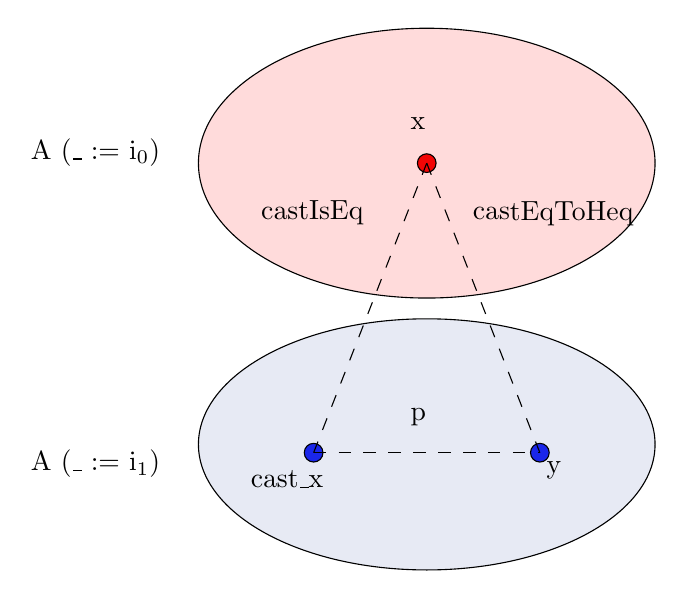
\begin{tikzpicture}[x=0.75pt,y=0.75pt,yscale=-1,xscale=1]
%uncomment if require: \path (0,300); %set diagram left start at 0, and has height of 300

%Shape: Ellipse [id:dp6858943436655307]
\draw  [fill={rgb, 255:red, 231; green, 234; blue, 244 }  ,fill opacity=1 ] (230,220.5) .. controls (230,187.09) and (279.25,160) .. (340,160) .. controls (400.75,160) and (450,187.09) .. (450,220.5) .. controls (450,253.91) and (400.75,281) .. (340,281) .. controls (279.25,281) and (230,253.91) .. (230,220.5) -- cycle ;
%Shape: Ellipse [id:dp4978096684614166]
\draw  [fill={rgb, 255:red, 255; green, 219; blue, 219 }  ,fill opacity=1 ] (230,85) .. controls (230,49.1) and (279.25,20) .. (340,20) .. controls (400.75,20) and (450,49.1) .. (450,85) .. controls (450,120.9) and (400.75,150) .. (340,150) .. controls (279.25,150) and (230,120.9) .. (230,85) -- cycle ;
%Shape: Circle [id:dp2462377080592002]
\draw  [fill={rgb, 255:red, 242; green, 5; blue, 5 }  ,fill opacity=1 ] (335.5,85) .. controls (335.5,82.51) and (337.51,80.5) .. (340,80.5) .. controls (342.49,80.5) and (344.5,82.51) .. (344.5,85) .. controls (344.5,87.49) and (342.49,89.5) .. (340,89.5) .. controls (337.51,89.5) and (335.5,87.49) .. (335.5,85) -- cycle ;
%Shape: Circle [id:dp1552015327211651]
\draw  [fill={rgb, 255:red, 26; green, 38; blue, 234 }  ,fill opacity=1 ] (390,224.5) .. controls (390,222.01) and (392.01,220) .. (394.5,220) .. controls (396.99,220) and (399,222.01) .. (399,224.5) .. controls (399,226.99) and (396.99,229) .. (394.5,229) .. controls (392.01,229) and (390,226.99) .. (390,224.5) -- cycle ;
%Shape: Circle [id:dp924511868212545]
\draw  [fill={rgb, 255:red, 26; green, 38; blue, 234 }  ,fill opacity=1 ] (281,224.5) .. controls (281,222.01) and (283.01,220) .. (285.5,220) .. controls (287.99,220) and (290,222.01) .. (290,224.5) .. controls (290,226.99) and (287.99,229) .. (285.5,229) .. controls (283.01,229) and (281,226.99) .. (281,224.5) -- cycle ;
%Straight Lines [id:da43777492366231496]
\draw  [dash pattern={on 4.5pt off 4.5pt}]  (285.5,224.5) -- (394.5,224.5) ;
%Straight Lines [id:da5251303335065973]
\draw  [dash pattern={on 4.5pt off 4.5pt}]  (340,85) -- (394.5,224.5) ;
%Straight Lines [id:da2553652396779533]
\draw  [dash pattern={on 4.5pt off 4.5pt}]  (340,85) -- (285.5,224.5) ;

% Text Node
\draw (331,62) node [anchor=north west][inner sep=0.75pt]   [align=left] {x};
% Text Node
\draw (396.5,227.5) node [anchor=north west][inner sep=0.75pt]   [align=left] {y};
% Text Node
\draw (254,232) node [anchor=north west][inner sep=0.75pt]  [font=\normalsize] [align=left] {cast\_x};
% Text Node
\draw (331,202) node [anchor=north west][inner sep=0.75pt]   [align=left] {p};
% Text Node
\draw (148,72) node [anchor=north west][inner sep=0.75pt]   [align=left] {A (\_ := i$_0$) };
% Text Node
\draw (148,222) node [anchor=north west][inner sep=0.75pt]   [align=left] {A (\_ := i$_1$) };
% Text Node
\draw (361,102) node [anchor=north west][inner sep=0.75pt]  [rotate=-0.06] [align=left] {castEqToHeq};
% Text Node
\draw (259,102) node [anchor=north west][inner sep=0.75pt]  [font=\normalsize] [align=left] {castIsEq};

\end{tikzpicture}

\end{center}

The circles represent the two types and points in the circle are elements of the
corresponding types. With our definition of equality, we can construct an
equality between $\Funapp{\id{A}}{(\earg{\_}{\ileft})}$ and
$\Funapp{\id{A}}{(\earg{\_}{\iright})}$ using \id{Eq\_eq}. Now, given that the
two circles are `equal', intuitively speaking, every point in one circle should
have a counterpart in the other circle, and this can be obtained by transporting a
point along the equality between the two types. Additionally, suppose also that
we have an equality between $\id{cast\_x}$ and $\id{y}$, this is indicated
by the path $\id{p}$ between the two points in the diagram. Given that $\id{x}$
is casted to $\id{cast\_x}$, and that $\id{cast\_x}$ is equal to
$\id{y}$, we also want to be able to say something about the relationship
between $\id{x}$ and $\id{y}$. Since they are not of the same type, all we can
do is construct a heterogeneous equality between them, and this is precisely
what the function $\id{castEqToHeq}$ seeks to do.

\begin{minted}[escapeinside=@@,mathescape=true]{agda}
    castEqToHeq : (A : I @$\Rrightarrow$@ Type) @$\Rrightarrow$@ (x : A (_ := @$\ileft$@)) @$\Rightarrow$@ (y : A (_ := @$\iright$@))
                  @$\Rightarrow$@ Eq_cast (p := Eq_eq (f := A)) (f := id) x @$\equiv$@ y
                  @$\rightarrow$@ Heq (t := A) x y
    castEqToHeq = @$\lambda$@ A @$\Rrightarrow$@ @$\lambda$@ x y @$\Rightarrow$@ @$\lambda$@ p @$\rightarrow$@
      whiskerRight (A := A) (castIsEq (A := A) x) p
\end{minted}

First, we construct a heterogeneous equality between $\id{x}$ and $\id{cast\_x}$
using the \id{castIsEq} lemma that we prove in \autoref{app:cast-is-eq}. Then,
we use the \id{whiskerRight} lemma described in \autoref{app:whiskering} of the
appendix to concatenate the above proof with \id{p} to produce a proof of
heterogeneous equality between \id{x} and \id{y}.

\begin{minted}[escapeinside=@@,mathescape=true]{agda}
elimProp : (P : Quotient ?A ?R @$\rightarrow$@ Type)
           @$\Rrightarrow$@ (prop : (x : Quotient ?A ?R) @$\rightarrow$@ isProp (P x))
           @$\rightarrow$@ (f : (x : ?A) @$\rightarrow$@ P (Quotient_in x))
           @$\rightarrow$@ (x : Quotient ?A ?R) @$\rightarrow$@ P x
elimProp prop f =
  Quotient_elim
    (R := R) (P := P) f
    (p := @$\lambda$@ a a' r @$\rightarrow$@
      let
        a=a' : Quotient_in (R := R) a @$\equiv$@ Quotient_in (R := R) a'
        a=a' = Quotient_eq (R := R) (a := a) (a' := a') r
        fa=fa' : Heq (f a) (f a')
        fa=fa' = castEqToHeq (A := @$\lambda$@ i @$\Rrightarrow$@ P (Eq_uneq (p := a=a') (i := i)))
                             (prop (Quotient_in a')
                                   (Eq_cast (p := a=a') (f := P) (f a))
                                   (f a'))
      in
        fa=fa')
\end{minted}

$\fn{castEqToHeq}$ does the heavy lifting in this proof by allowing us to leverage $\Funapp{\fn{isProp}}{(\Funapp{\id{P}}{\id{x}})}$ to easily produce a proof of $\Funapp{\id{Heq}}{(\Funapp{\id{f}}{\id{a}})}{(\Funapp{\id{f}}{\id{a}'})}$. We can also iterate this to define $\fn{elimProp}_2$, $\fn{elimProp}_3$ etc. In general, we can define $\fn{elimProp}_n$ in terms of $\fn{elimProp}_{n-1}$ and $\fn{elimProp}$. To illustrate this, we define $\fn{elimProp}_2$.

\begin{minted}[escapeinside=@@,mathescape=true]{agda}
elimProp2 : (P : Quotient ?A ?R @$\rightarrow$@ Quotient ?B ?S @$\rightarrow$@ Type)
            @$\Rrightarrow$@ (prop : (x : Quotient ?A ?R) @$\rightarrow$@ (y : Quotient ?B ?S)
                       @$\rightarrow$@ isProp (P x y))
            @$\rightarrow$@ (f : (x : ?A) @$\rightarrow$@ (y : ?B) @$\rightarrow$@ P (Quotient_in x) (Quotient_in y))
            @$\rightarrow$@ (x : Quotient ?A ?R) @$\rightarrow$@ (y : Quotient ?B ?S) @$\rightarrow$@ P x y
elimProp2 prop f =
  elimProp (P := @$\lambda$@ x @$\rightarrow$@ (y : Quotient B S) @$\rightarrow$@ P x y)
           (@$\lambda$@ x @$\rightarrow$@ isProp@$\Pi$@ (B := P x) (prop x))
           (@$\lambda$@ a @$\rightarrow$@ elimProp (P := P (Quotient_in a))
                            (prop (Quotient_in a)) (f a))
\end{minted}

We make use of \id{isProp$\Pi$}, a lemma that states that the property of being
a mere proposition is closed under the $\Pi$ type former. A proof of this is
provided in \autoref{app:closure-mp-pi} of the appendix.

\section{Functional Extensionality}\label{sec:quot-implies-funext}

In intensional type theory, functional extensionality is a property that is
respected by all functions, however, typically this may not be proven. In this
section, we demonstrate that the existence of quotient types implies functional
extensionality. Note that this proof requires quotient types, and not normalised
types which are a strict subset of quotient types.

\begin{minted}[escapeinside=@@,mathescape=true]{agda}
funext : (A : Type) @$\rightarrow$@ (B : A @$\rightarrow$@ Type)
         @$\rightarrow$@ (f1 f2 : (a : A) @$\rightarrow$@ B a) @$\rightarrow$@ (h : (a : A) @$\rightarrow$@ f1 a @$\equiv$@ f2 a)
         @$\rightarrow$@ f1 @$\equiv$@ f2
funext A B f1 f2 h =
  let
    fn_type = (a : A) @$\rightarrow$@ B a

    equiv_rel : fn_type @$\rightarrow$@ fn_type @$\rightarrow$@ Type
    equiv_rel f1 f2 = ((a : A) @$\rightarrow$@ f1 a @$\equiv$@ f2 a)

    extfun_app : Quotient fn_type equiv_rel @$\rightarrow$@ fn_type
    extfun_app f a = Quotient_rec (R := equiv_rel)
                                  (f := @$\lambda$@ f @$\rightarrow$@ f a)
                                  (p := @$\lambda$@ f1 f2 r @$\rightarrow$@ r a) f

    sound : Quotient_in (R := equiv_rel) f1 @$\equiv$@ Quotient_in (R := equiv_rel) f2
    sound = Quotient_eq (R := equiv_rel) (a := f1) (a' := f2) h

  in
    Eq_cong extfun_app sound
\end{minted}

We quotient functions by a relation \id{equiv\_rel} that represents pointwise
equality. By making use of the $\beta$-rule of \id{Quotient\_rec} and the
$\eta$-equivalence of functions, we construct the desired proof by using the
congruence property of equality.

\chapter{Quotient Effectiveness}\label{ch:quotient-effectiveness}

We show that if it is the case that two projections of two terms into a quotient
are equal, i.e. \fn{Quotient_in (R := R) a $\equiv$ Quotient (R := R) a'}, then
the two terms \id{a} and \id{a'} must necessarily be related under the relation.
In other words, we want to show that the reverse of
\hyperref[quot-intro-eq-rule]{\textsc{Quot-Intro-Eq}} is also valid. We note
however that this is only valid for relations that are equivalence relations
(i.e.\ reflexive, symmetric, and transitive).

\section{Propositional Extensionality}
We provide an alternative version of propositional extensionality that is
slightly weaker. Consequently, the version of quotient effectiveness that we
prove is also weaker.

\subsection*{Representation of propositions}\label{subsec:mere-propositions}

Intuitively speaking, mere propositions are a type that contain no intrinsic
data, it is their mere existence that counts. This is precisely the notion of
proof irrelevance. In Typer, one way of representing this notion is via
erasability. We introduce a built-in data type that captures this idea.

\begin{minted}{agda}
    type Erased (T : Type)
      | erased (t ::: T)
\end{minted}

By ensuring that the witness $\id{t}$ of the type $\id{T}$ is erasable, this
provides us with a guarantee that during elimination, the witness $\id{t}$ can
only be used in an erasable, i.e.\ proof irrelevant manner.

%% FIXME: This would no longer work without conv_erase!
%% I guess we just have to live without this proof?

%% To convince ourselves that this type does indeed capture the essence of a
%% mere proposition, we provide a proof of
%% $\Funapp{\id{isProp}}{(\Funapp{\id{Erased}}{?\id{T}})}$. We first state the
%% definition of $\id{isProp}$:

%% \begin{minted}[escapeinside=||,mathescape=true]{agda}
%% isProp : (T : Type) |$\rightarrow$| Type
%% isProp T = (x y : T) |$\rightarrow$| Eq x y
%% \end{minted}

%% We now present the proof in the form of Typer code.

%% \begin{minted}[escapeinside=@@,mathescape=true]{agda}
%% erasedIsProp : (T : Type) @$\Rrightarrow$@ isProp (Erased T)
%% erasedIsProp t1 t2 =
%%   case t1
%%     | erased (_ := e1) @$\Rightarrow$@
%%         let
%%           p1 = ##DeBruijn 0 : Eq (erased (t := e1)) t1
%%         in
%%           case t2
%%             | erased (_ := e2) @$\Rightarrow$@
%%                 let
%%                   p2 = ##DeBruijn 0 : Eq (erased (t := e2)) t2
%%                 in
%%                   Eq_trans (Eq_comm p1) p2
%% \end{minted}

%% Typer does not offer the direct specialisation of $\kw{case}$ targets in
%% branches. In other words, in the first case branch, we do not have a
%% definitional equality between $\id{t1}$ and
%% $\Funapp{\id{erased}}{(\earg{\_}{\id{e1}})}$. Instead, an equality proof between
%% them is injected into the context, which can be accessed as the variable at
%% deBruijn index 0. Now that we have the two equality proofs, to
%% concatenate them\footnote{By considering equalities as paths, the application of
%% the transitivity property of equality is conceptually similar to concatenating
%% two paths.}, we require $\Funapp{\id{erased}}{(\earg{\_}{\id{e1}})}$ and
%% $\Funapp{\id{erased}}{(\earg{\_}{\id{e2}})}$ to be equal. A priori, the two
%% terms are not equal as $\id{e1}$ and $\id{e2}$ are completely arbitrary.
%% However, Typer ignores erasable terms when checking the convertibility of terms,
%% this is a property that was proven to be sound in\cite{barras2008implicit} as
%% convertibility is tested on extracted terms. This allows the concatenation to
%% succeed and thus concludes the proof.

\subsection*{Implementation details}

Propositional extensionality essentially means that if two logically equivalent
propositions, i.e.\ each proposition implies the other, then we can say that
they are equal. And precisely because we are postulating a new equality
constructor, we have to be very careful that the resulting equality proof is
indeed proof irrelevant. In other words, we need this equality proof to not have
any run-time relevance. This is principally because we insist that the transport
operation be a no-op during run time. This is the motivation behind our choice to
use the $\id{Erased}$ type to represent propositions, as it is a guarantee that
such a type carries no useful run-time information. This implies that a transport
operation from one $\id{Erased}$ type to another is necessarily simply a no-op.

In a setting with univalence, propositional extensionality is simply a theorem
that may be proven, more specifically, it may be seen as a degenerate case of univalence\cite{sozeau2013univalence}. This is a result that is
immediate as an equivalence between logically equivalent propositions is
trivial. In the setting of Typer, however, propositional extensionality is
implemented as an axiom with the following type signature:

\begin{minted}[escapeinside=@@,mathescape=true]{agda}
propExt : (Erased ?A @$\rightarrow$@ Erased ?B) @$\rightarrow$@ (Erased ?B @$\rightarrow$@ Erased ?A)
          @$\rightarrow$@ Erased ?A @$\equiv$@ Erased ?B
\end{minted}

The above is a weaker notion of propositional extensionality compared to what is
proposed in Cubical Agda, which has the following type signature:

\begin{minted}[escapeinside=@@,mathescape=true]{Agda}
propExt : {A B : Type} @$\rightarrow$@ isProp A @$\rightarrow$@ isProp B @$\rightarrow$@ (A @$\rightarrow$@ B) @$\rightarrow$@ (B @$\rightarrow$@ A) @$\rightarrow$@ A @$\equiv$@ B
\end{minted}

However, this produces an equality proof that is not proof irrelevant, as
$\id{A}$ and $\id{B}$ are not necessarily the \emph{same} type. We illustrate
the above with a simple example. We define two instances of the unit type which
are trivially \emph{logically equivalent}.

\begin{minted}[escapeinside=@@,mathescape=true]{Agda}
    data Unit1 : Type where
      unit1 : Unit1

    data Unit2 : Type where
      unit2 : Unit2
\end{minted}

$\Funapp{\id{isProp}}{\id{Unit1}}$ and $\Funapp{\id{isProp}}{\id{Unit2}}$ are
trivially true, as is the case for all $\mathbb{1}$-types\footnote{Types with
exactly one inhabitant.}. $\id{Unit1} \rightarrow \id{Unit2}$ and $\id{Unit2}
\rightarrow \id{Unit1}$ are also inhabited. Propositional extensionality thus
gives us a proof of $\id{Unit1} \equiv \id{Unit2}$. This implies that we should
be able to use said proof to transport $\id{unit1}$ to $\id{unit2}$, but since
the two terms do not have the same run-time representation, this simply cannot be
a no-op. This is in stark contrast to the version of propositional extensionality
that we are proposing in Typer which only accepts types that are boxed in the
$\id{Erased}$ type. We would have no qualms about having a proof of equality
between $\Funapp{\id{Erased}}{\id{Unit1}}$ and
$\Funapp{\id{Erased}}{\id{Unit2}}$ as terms of these two types would essentially
have the same run-time representation. It is also for this precise reason that
our version of propositional extensionality is weaker, as we are constrained to
construct an equality proof that is not computationally relevant.

Another worthy comparison to make is with \Lean{}, which has a $\kw{Prop}$ sort.
Terms of this sort are not authorised to be used in a proof-relevant manner. Its
version of propositional extensionality has the following form:

\begin{minted}[escapeinside=@@,mathescape=true]{lean}
    axiom propext {a b : Prop} : (a @$\leftrightarrow$@ b) @$\rightarrow$@ a = b
\end{minted}

This is similar to what we have in Typer, except that proof irrelevance is
enforced differently.

\section{Equivalence relation}

First, we state what we mean when we say \emph{relation} to set the stage for
the subsequent discussion. For our purposes, we consider binary relations, which
are type formers that take two arguments of some type $\id{A}$. Assuming that we
call the relation $\id{R}$ and its two arguments $\id{a}$ and $\id{a}'$
respectively, inhabitants of the type $\Funapp{\id{R}}{\id{a}}{\id{a}'}$ are
witnesses of this binary relation. The type signature of a binary relation has
the below form:

\begin{minted}[escapeinside=||,mathescape=true]{agda}
    R : (a : ?A) |$\rightarrow$| (a' : ?A) |$\rightarrow$| Type
\end{minted}

For a quotient to be effective, its underlying relation has to be an equivalence
relation, we shall use this property in the proof in the subsequent section.
Recall that an equivalence relation implies that the relation is reflexive,
symmetric and transitive. For it to be reflexive, it needs to be the case that
given an arbitrary $\oftype{\id{a}}{\id{A}}$, $\Funapp{\id{R}}{\id{a}}{\id{a}}$
must be trivially inhabited. The symmetry of the relation implies that if we are
given an arbitrary witness of $\Funapp{\id{R}}{\id{a}}{\id{a}'}$, we need to be
able to transform that into an inhabitant of $\Funapp{\id{R}}{\id{a}'}{\id{a}}$.
The relation is transitive if we are able to transform witnesses of
$\Funapp{\id{R}}{\id{a}}{\id{b}}$ and $\Funapp{\id{R}}{\id{b}}{\id{c}}$ into
witnesses of $\Funapp{\id{R}}{\id{a}}{\id{c}}$\footnote{The equality type
fulfills these criteria and is an equivalence relation.}.

In the built-in library, we define the following type as a witness that a
certain relation is indeed an equivalence relation.

\begin{minted}[escapeinside=@@,mathescape=true]{agda}
    type isEquivRel (A : Type) (R : A @$\rightarrow$@ A @$\rightarrow$@ Type) : Type
      | equivRel (isRefl : (a : A) @$\rightarrow$@ R a a)
                 (isSym : (a b : A) @$\rightarrow$@ R a b @$\rightarrow$@ R b a)
                 (isTrans : (a b c : A) @$\rightarrow$@ R a b @$\rightarrow$@ R b c @$\rightarrow$@ R a c)
\end{minted}

\section{Proof}
Given two arbitrary elements $\id{a}$ and $\id{a}'$ of a base type $\id{A}$, a
quotient is said to be effective if given a proof that the projection of $\id{a}$
and $\id{a}'$ into the quotient are equal, then it must be the case that
$\Funapp{\id{R}}{\id{a}}{\id{a}'}$ is true, i.e.\ we are able to find an
inhabitant of it. A sufficient condition for a quotient to be effective is that
the underlying relation must be an equivalence relation.

For an arbitrary binary relation $\id{R}$, we can define the following:

\begin{minted}[escapeinside=||,mathescape=true]{agda}
    ErasedR : (?A |$\rightarrow$| ?A |$\rightarrow$| Type) |$\rightarrow$| ?A |$\rightarrow$| ?A |$\rightarrow$| Type
    ErasedR R a b = Erased (R a b)
\end{minted}

Now, we state the proof of the effectiveness of quotients in the form of Typer code

\begin{minted}[escapeinside=||,mathescape=true]{agda}
effective : isEquivRel ?A (ErasedR ?R) |$\rightarrow$| (a b : A)
            |$\rightarrow$| Quotient_in (R := ErasedR R) a |$\equiv$| Quotient_in (R := ErasedR R) b
            |$\rightarrow$| ErasedR R a b
effective equiv a b eq =
  let
    helper : Quotient A (ErasedR R) |$\rightarrow$| Type
    helper x =
      Quotient_rec
        (R := ErasedR R)
        (|$\lambda$| |$\rightarrow$| ErasedR R a c)
        (p := |$\lambda$| c d cd |$\rightarrow$|
          let
            ac|$\rightarrow$|ad : Erased (R a c) |$\rightarrow$| Erased (R a d)
            ac|$\rightarrow$|ad ac = equiv.isTrans a c d ac cd
            ad|$\rightarrow$|ac : Erased (R a d) |$\rightarrow$| Erased (R a c)
            ad|$\rightarrow$|ac ad = equiv.isTrans a d c ad
                                      (equiv.isSym c d cd)
          in
            propExt ac|$\rightarrow$|ad ad|$\rightarrow$|ac)
        x
    aa=ab : Erased (R a a) |$\equiv$| Erased (R a b)
    aa=ab = Eq_cong helper eq
  in
    Eq_cast (p := aa=ab) (f := id) (equiv.isRefl a)
\end{minted}

Compared to the more general version of the theorem we stated before, here we
insist that the quotient we consider be based on the erased version of some
binary relation $\id{R}$. And instead of proving that the base relation itself
holds for some $\id{a}$ and $\id{b}$, we can only show that the erased version
of this relation holds.

In this proof, we can see that all aspects of the sufficient condition are at
play. It is mainly used to prove that for arbitrary terms $\id{a}$, $\id{b}$ and
$\id{c}$ of type $\id{A}$, if it is the case that if
$\Funapp{\id{Erased}}{(\Funapp{\id{R}}{\id{b}}{\id{c}})}$ is inhabited, then
$\Funapp{\id{Erased}}{(\Funapp{\id{R}}{\id{a}}{\id{b}})}$ $\iff$
$\Funapp{\id{Erased}}{(\Funapp{\id{R}}{\id{a}}{\id{c}})}$. Intuitively speaking
this makes a lot of sense,
$\Funapp{\id{Erased}}{(\Funapp{\id{R}}{\id{b}}{\id{c}})}$ implies that $\id{b}$
and $\id{c}$ are in the same equivalence class of the quotient. Hence, if we
know that $\id{a}$ is in the same equivalence class as $\id{b}$, we should
naturally be able to infer that $\id{a}$ and $\id{c}$ are also in the same
equivalence class, and vice versa. Propositional extensionality takes us even
further, by allowing us to prove that
$\Funapp{\id{Erased}}{(\Funapp{\id{R}}{\id{a}}{\id{b}})}$ and
$\Funapp{\id{Erased}}{(\Funapp{\id{R}}{\id{a}}{\id{c}})}$ are equal since they
are both mere propositions.

\chapter{Evaluation}\label{ch:evaluation}

At the start of this work, we first set out to augment Typer with a more
powerful and expressive notion of equality. We achieved this by basing our new
equality type on an Interval type. We showed the benefits of such an equality
type by demonstrating that the manipulation of propositional equality is greatly
simplified. To that end, we illustrated the derivation of various
equality-related theorems in a clean and elegant manner. Some desirable
properties such as functional extensionality that we are now able to derive were
previously unprovable by using Typer's original equality type.

We then introduced quotient types to Typer. We convinced ourselves that our
quotient types behave as they should by proving that they fulfil the universal
property of quotients. We note as well that our dependent elimination of
quotients is not limited to motives that live in the universe of \type{Prop},
as opposed to when quotient types are added to a theory interpreted in a setoid
model as proposed by Li\cite{li2015quotient} as well as the implementation in
\Lean{} described in \autoref{sec:intro-lean-quotients}. A library was provided
with proofs of many other properties fulfilled by our quotient types. We also
explored the practical aspects of our quotient types by using them to construct
several examples. We then observed that when the identifications that we wish
to impose on the base type may be immediately represented as an equivalence
relation, the resulting construction was a lot simpler as was the case with
\id{Rational}. However, our experience constructing \id{Multiset} in
\autoref{sec:multiset} showed that when the identifications that we require do
not immediately induce an equivalence relation, we need to manually construct
the equivalence closure of the resulting relation. This complicates the
underlying relation of the quotient, leading to additional proof obligations
that are often easily satisfied but unnecessary. This may be seen as a glaring
disadvantage of our approach as opposed to QITs that allow the direct
definition of path constructors on inductive types. We initially intended to
encode QITs as quotient types with the help of a macro, however, we then
realised that the construction of the equivalence closure of arbitrary equality
constructors using a macro is non-trivial. Hence, we ultimately decided to
abandon this idea as even if such a macro were to come to fruition, it would
most likely be user-unfriendly.

HITs and QITs are also strictly more expressive than the combination of ordinary
inductive types with quotient types\cite{fiore2022quotients}. This implies that
our above endeavour to encode QITs as quotient types was not a feasible task to
begin with. In practice, we think that the additional expressivity is often
unrequired for general programming. The example provided by the aforementioned
paper of a QIT that we may not trivially define using quotient types in the form
of unordered infinitely branching trees is indeed not a data type that one would
expect to make a frequent appearance in daily programming tasks. The simpler
implementation of our quotient types thus gives us the benefit of preserving the
modularity of the existing implementation of inductive types in Typer while
providing users with the power of quotients.

\section*{Proof Obligations of Quotient Types}

As the examples in the previous sections would suggest, the usage of quotient
types is often accompanied by a considerable amount of proof obligations. As we
have seen, such proofs are not always trivial to construct, mainly because of
Typer's current lack of support for the development of proofs as opposed to
other contemporary programming languages. For instance, the Quotient Haskell
extension\cite{hewer2023quotient} is implemented with the help of SMT solvers.
This enables many proof obligations generated by quotient types to be satisfied
automatically. In other words, most of the proofs that we had to write by hand
in \autoref{ch:quot-examples} while constructing the types \id{Rational} and
\id{Multiset} could have been solved automatically without too much hassle. The
proof development experience can also be contrasted to interactive proof
assistants that feature tactics such as \Coq{} and \Lean{}. Tactics generally
allow us to write our proofs in a less verbose manner by preventing unnecessary
repetition. Most of our long chains of equational reasoning involved the
repeated application of the congruence property of equality. This is analogous
to the usage of the \emph{rewrite} tactics of the aforementioned proof
assistants with the difference that invocation of \id{Eq\_cong} requires us to
manually specify the context in which the rewrite should occur. The more
verbose proofs are more readable in certain situations by allowing intermediate
steps of the proof to be explicitly stated, although this is not always the
case. The added verbosity makes their development a laborious endeavour. During
the construction of \id{Rational}, we had to do a lot of monotonous reasoning
related to linear arithmetic to prove propositions that were seemingly obvious
to the human eye. Such goals may typically be solved using tactics such as
\Coq{}'s \kw{lia} tactic and \Lean{}'s \kw{linarith} tactic that are
essentially solvers for linear goals over $\mathbb{Z}$. For the moment, Typer
also lacks the powerful dependent pattern-matching system of \Agda{}. This
inconvenience is somewhat mitigated by the presence of the
\fn{\kw{case}...\kw{return}...} construct that is reminiscent of \Coq{}.
However, just like \Coq{}, while we are in \kw{case} branches, we still lack
the specialisation of types of other variables in the context that depend on
the scrutinee. This was an inconvenience that we had to reckon with on numerous
occasions while working with quotient types. The above seems to be desirable
features that we should contemplate introducing to Typer in some shape or form
to facilitate proof development.

\section*{Computational Behaviour}\label{sec:eval-computation-behaviour}

The introduction of \id{Quotient\_eq} as an axiom also leads to the absence of a
desirable computational property. Suppose that the following terms \fn{a :\@ A},
\fn{a' :\@ A}, and \fn{r :\@ R a a'} as well as a function \fn{f :\@ A $\rightarrow$
  B} and a proof that it respects the relation \id{R}, i.e.\ \fn{p :\@ (a a' :\@ A)
  $\rightarrow$ R a a' $\rightarrow$ f a $\equiv$ f a'}. Unfortunately, the
following equality does not hold definitionally \fn{Eq\_cong (Quotient\_rec f (p
  := p)) (Quotient\_eq r) $\equiv$ p a a' r}. This would indeed be a
definitional equality in Cubical Agda if we were to use the construction that
was shown in \autoref{sec:cubical-agda}. However, it was not clear to us how the
same could be done in Typer as it would involve the hard coding of this
equivalence in an ad hoc manner.

The traditional approach of adding functional extensionality to an ITT as an
axiom breaks canonicity (introduced in \autoref{sec:intro-lean-quotients}).
This is because the transport function does not know how to compute on
arbitrary equality proofs. Fortunately for us, our new implementation of
equality has a transport function that computes not on the proof term itself,
but on the two types involved in the cast. For instance, the example given
in\cite{altenkirch2007observational} involving a cast on an equality proof
constructed by functionality extensionality does not lead to a stuck term in
our system as shown in the following code snippet:

\begin{minted}[escapeinside=@@,mathescape=true]{agda}
    plus0 : (x : Nat) @$\rightarrow$@ zero + x @$\equiv$@ x + zero
    plus0 x = Nat+_comm zero x

    eqf = Eq_funext (f := @$\lambda$@ x @$\rightarrow$@ zero + x) (g := @$\lambda$@ x @$\rightarrow$@ x + zero) plus0

    canon0 : Eq_cast (p := eqf) (f := @$\lambda$@ _ @$\rightarrow$@ Nat) zero @$\equiv$@ zero
    canon0 = Eq_refl
\end{minted}

\id{plus0} is a proof that both ways of adding \id{zero} to an integer \id{x}
are equal since the addition of natural numbers is commutative. This is a
witness that the two functions that are passed to \id{Eq\_funext} are
extensionally equal, allowing us to use functional extensionality to construct
an equality proof between them. The implementation of \kw{cast} in proof
assistants that implement ITT typically only reduces on reflexive proofs of
equality. This implies that a term such as \fn{Eq\_cast (p := eqf) (f :=
$\lambda$ \_ $\rightarrow$ Nat) zero} would not reduce to \id{zero} despite the
fact that this cast does not even utilise the proof constructed by
\id{Eq\_funext} as the motive \id{f} does not use its argument. For instance,
this problem would occur in \Lean{}, regardless of whether we define functional
extensionality as an axiom or if we derive it as a theorem from quotient types
as we did in \autoref{sec:quot-implies-funext}. Our implementation of \kw{cast}
recognises the fact that we are performing a cast between two definitionally
equal types, i.e., \id{Nat} and \id{Nat}, and thus successfully reduces. i.e.,
\id{Nat} and \id{Nat}, and thus successfully reduces \fn{Eq_cast (p := eqf) (f
:= $\lambda$ _ $\rightarrow$ Nat) zero} to \id{zero}. This is another one of
the benefits of our interval-based equality type.

However, this is not without its pitfalls. Consider the below example:

\begin{minted}[escapeinside=@@,mathescape=true]{agda}
    type NatFnPred (f : Nat @$\rightarrow$@ Nat)
      | natFnPred

    np1 : NatFnPred (@$\lambda$@ x @$\rightarrow$@ zero + x)
    np1 = natFnPred

    np2 : NatFnPred (@$\lambda$@ x @$\rightarrow$@ x + zero)
    np2 = Eq_cast (p := eqf) (f := NatFnPred) np1
\end{minted}

Here, the motive \id{f} does make use of its argument. Since \fn{NatFnPred
($\lambda$ x $\rightarrow$ zero + x)} and \fn{NatFnPred ($\lambda$ x
$\rightarrow$ x + zero)} are not definitionally equal, \id{np2} is a stuck
term, i.e., it does not reduce to \id{natFnPred}, the only constructor of its
type. This implies that canonicity is not preserved for all types. We could
also construct a similar example using \id{Quotient_eq} by constructing a type
family indexed by a quotient type. Unfortunately, we were not able to find a
satisfactory solution to this problem; hence, we leave it for future work.

\section*{Benchmarks}\label{sec:quot-benchmark}

In this section, we use our implementation of \id{Rational} and \id{Multiset}
to explore the run-time cost of using quotient types in Typer. Quotient types
are nothing more than a means of using the type system to ensure that
programmers respect a certain relation on a base type through proof
obligations. By carefully setting things up so that these proofs are always
erasable, we can expect them to be absent in the generated code. As a result,
we hope for quotient types to be a zero-cost abstraction at run time. The tests
in our benchmark were designed to help us identify the overhead cost of using
quotient types (if any) and what we need to do to mitigate it.

\subsection*{Rational}

Since the operations on rational numbers are essentially wrappers around
operations on the base type $\zpair$, our benchmark simply compares the
execution time of operations on $\zpair$ with their $\fn{Rational}$
counterparts\footnote{The code for this may be found in the
\href{https://gitlab.com/jamestjw/typer/-/blob/quot-types-v1.0.0/samples/rational_benchmark.typer}{\id{samples/rational\_benchmark.typer}}
file.}. We examine the run-time cost\footnote{The tests were executed on the
author's 2018 Macbook Pro with a quadcore 2.3GHz Intel Core i5 processor with
8GB of RAM.} of executing the functions $\fn{Rational\_negate}$,
$\fn{Rational\_+}$, $\fn{Rational\_-}$ and $\fn{Rational\_*}$ on 50000 pairs of
rational numbers with 100 iterations. We also ensured that we only used
integers that fit within the 63-bit limit of the OCaml standard library's
integer type to avoid the use of heap-allocated integers. We then report the
average execution time over the 100 iterations along with the standard
deviation. The overhead is defined to be the difference in the average
execution time.

%% SM: Personally I find the overhead to make more sense when expressed
%% as a percentage.
\begin{table}[]
\centering
\begin{tabular}{@{}ccccccc@{}}
\toprule
\multirow{3}{*}{Operation} & \multicolumn{4}{c}{Execution Time (seconds)}                         & \multicolumn{2}{c}{Overhead}                   \\ \cmidrule(l){2-7}
                           & \multicolumn{2}{c}{Average} & \multicolumn{2}{c}{Standard Deviation} & \multirow{2}{*}{seconds} & \multirow{2}{*}{\%} \\
               & $\zpair$ & Rational & $\zpair$ & Rational &        &      \\ \midrule
Negation       & 0.2825   & 0.3872   & 0.0272   & 0.0201   & 0.1047 & 37.0 \\
Addition       & 0.5268   & 0.8354   & 0.0308   & 0.0415   & 0.3086 & 58.6 \\
Subtraction    & 0.6899   & 1.1180   & 0.0411   & 0.0286   & 0.4281 & 62.1 \\
Multiplication & 0.4877   & 0.8000   & 0.0346   & 0.0372   & 0.3123 & 64.0 \\ \bottomrule
\end{tabular}
\caption{The run-time cost of operations on rational numbers with and without the
  use of quotient types.}\label{tab:rational-benchmark}
\end{table}

We observe that there is a non-negligible overhead caused by the usage of
quotient types, which we will now try to justify. Without loss of generality, we
discuss the addition operation. Once the $\zpairplus$ function that handles the
addition of $\zpair$ and its $\fn{Rational}$ counterpart, $\fn{Rational\_+}$
have undergone erasure, the resulting functions are extensionally equal. By
definition of erasure\cite{monnier2019typer}, all erasable arguments are
removed, hence all proof objects required by the quotient type will be absent in
the erased versions of the above functions. The two erased functions are
nevertheless not completely equal, as we shall see by examining the Elexp
(erased lambda expression)\cite{delaunay2017implementation} of
$\fn{Rational\_+}$:

\begin{minted}[escapeinside=@@,mathescape=true]{scheme}
    (@$\lambda$@ (a) @$\rightarrow$@ (@$\lambda$@ (b) @$\rightarrow$@
      (Quotient_rec2 (@$\lambda$@ (x) @$\rightarrow$@ (@$\lambda$@ (y) @$\rightarrow$@ Quotient_in (@$\zpairplus$@ x y)))
                     a b)))
\end{minted}

Through a series of $\eta$-reductions and inlinings, we can see that the above
expression is equivalent to $\zpairplus$.

\begin{figure}
\begin{mdframed}
\begin{minted}[escapeinside=@@,mathescape=true]{scheme}
    (@$\lambda$@ (a) @$\rightarrow$@ (@$\lambda$@ (b) @$\rightarrow$@
      (Quotient_rec2 (@$\lambda$@ (x) @$\rightarrow$@ (@$\lambda$@ (y) @$\rightarrow$@ Quotient_in (@$\zpairplus$@ x y)))
                     a b)))

        @$\leadsto$@ @$\eta$@-reduction of lambdas

    Quotient_rec2 (@$\lambda$@ (x) @$\rightarrow$@ (@$\lambda$@ (y) @$\rightarrow$@ Quotient_in (@$\zpairplus$@ x y)))

        @$\leadsto$@ Inlining of Quotient_rec2

    Quotient_rec (@$\lambda$@ (a) @$\rightarrow$@
        Quotient_rec ((@$\lambda$@ (x) @$\rightarrow$@ (@$\lambda$@ (y) @$\rightarrow$@ Quotient_in (@$\zpairplus$@ x y))) a))

        @$\leadsto$@ Inlining of Quotient_rec

    (@$\lambda$@ (a) @$\rightarrow$@
        Quotient_rec ((@$\lambda$@ (x) @$\rightarrow$@ (@$\lambda$@ (y) @$\rightarrow$@ Quotient_in (@$\zpairplus$@ x y))) a))

        @$\leadsto$@ Inlining of Quotient_rec

    (@$\lambda$@ (a) @$\rightarrow$@ (@$\lambda$@ (x) @$\rightarrow$@ (@$\lambda$@ (y) @$\rightarrow$@ Quotient_in (@$\zpairplus$@ x y))) a)

        @$\leadsto$@ @$\eta$@-reduction of lambdas

    (@$\lambda$@ (x) @$\rightarrow$@ (@$\lambda$@ (y) @$\rightarrow$@ Quotient_in (@$\zpairplus$@ x y)))

        @$\leadsto$@ Inlining of Quotient_in

    (@$\lambda$@ (x) @$\rightarrow$@ (@$\lambda$@ (y) @$\rightarrow$@ @$\zpairplus$@ x y))

        @$\leadsto$@ @$\eta$@-reduction of lambdas

    @$\zpairplus$@
\end{minted}
\end{mdframed}
\caption{Proposed optimisations for \id{Rational\_+}}\label{fig:optim-rational-add}
\end{figure}

A desirable optimisation is the inlining of \id{Quotient\_in}, \id{Quotient\_rec} and
\id{Quotient\_rec2} as follows:

\begin{itemize}
  \item{\fn{Quotient\_in e} $\leadsto$ \id{e}}

  \item{\fn{Quotient\_rec f} $\leadsto$ \id{f}}

  \item{\fn{Quotient\_rec2 f} $\leadsto$ \fn{Quotient\_rec ($\lambda$ a $\rightarrow$ Quotient\_rec (f a))}}
\end{itemize}

We also would require a multi-argument version of the $\eta$-reduction rule for
lambda functions like so:

\begin{itemize}
  \item{\fn{($\lambda$ (e$_1$) ($\lambda$ (e$_2$) ... ($\lambda$ (e$_n$) f e$_1$ e$_2$ ... e$_n$))) $\leadsto$ f}}
\end{itemize}

With that, we show a possible series of reductions and optimisations that
simplify \fn{Rational\_+} to $\zpairplus$ in \autoref{fig:optim-rational-add}.
This implies that with an appropriate optimisation phase, Elexps containing
quotient primitives could be simplified to completely neutralise the overhead of
quotient types. We would also like to point out that as far as optimisations go,
our propositions are fairly standard, we thus leave them for future work. These
optimisations are indeed rather desirable as we have observed that incurred
overhead increases the execution time by up to a 64\% in the case of the simple
operations that we investigated.

We believe that the incurred overhead for these operations should be a constant
cost based on whether the operation is defined using \id{Quotient\_rec} or
\id{Quotient\_rec2}. Since \id{Quotient\_rec2} is defined in terms of
\id{Quotient\_rec}, \id{Quotient\_rec2} logically incurs a larger overhead than
\id{Quotient\_rec}. \id{Rational\_negate} being a unary function, was the only
one that was defined using \id{Quotient\_rec}, and thus suffers from the least
amount of overhead. \id{Rational\_+} and \id{Rational\_*} were both defined
using \id{Quotient\_rec2}, hence we observe how the two operations have a
similar overhead. Since we defined \id{Rational\_-} based on \id{Rational\_+}
combined with \id{Rational\_negate}, it is well justified that its overhead is
similar to the combined overhead of the two operations that it was defined on.

\subsection*{Multiset}

We do a similar set of experiments on our construction of \id{Multiset} with the
\id{Multiset\_append} and \id{Multiset\_mem} operations.

\begin{table}[]
\centering
\begin{tabular}{@{}ccccccc@{}}
\toprule
\multirow{3}{*}{Operation} & \multicolumn{4}{c}{Execution Time (seconds)}                         & \multicolumn{2}{c}{Overhead}                   \\ \cmidrule(l){2-7}
                           & \multicolumn{2}{c}{Average} & \multicolumn{2}{c}{Standard Deviation} & \multirow{2}{*}{seconds} & \multirow{2}{*}{\%} \\
       & List   & Multiset & List   & Multiset &        &      \\ \midrule
Append & 1.3081 & 1.5472   & 0.0497 & 0.0516   & 0.2390 & 18.3 \\
Member & 0.8417 & 0.8730   & 0.0278 & 0.0227   & 0.0314 & 3.7  \\ \bottomrule
\end{tabular}
\caption{The run-time cost of operations on multisets with and without the use of quotient types.}\label{tab:benchmark-multiset}
\end{table}

The \id{Multiset\_append} operation was tested by appending multisets containing
25 integers 50000 times. For the \id{Multiset\_mem} operation, we ran the
membership test with 50000 integers on a multiset containing 10 integers. For
lists, we ran the benchmark using the \id{List\_mem} function that we show
below. We ran 100 iterations for each experiment and like before, we report the
average execution time along with the standard deviation.

\begin{minted}[escapeinside=@@,mathescape=true]{agda}
    List_mem : Discrete ?A @$\rightarrow$@ ?A @$\rightarrow$@ List ?A @$\rightarrow$@ Bool
    List_mem disc a l = Dec2Bool (isMemberDec disc a l)
\end{minted}

We observe that the average overhead cost of \id{Multiset\_append} is similar to
the cost incurred by \id{Rational\_+} and \id{Rational\_*} as
\id{Multiset\_append} was defined in a largely similar manner using
\id{Quotient\_rec2}. We then compare \id{Multiset\_mem} and
\id{Rational\_negate} since they were both defined using \id{Quotient\_rec}. We
observe, however, that the overhead cost of \id{Multiset\_mem} is less than
\id{Rational\_negate}. We believe that this is because unlike
\id{Rational\_negate}, \id{Multiset\_mem} does not construct a new quotient term
as it returns a \id{Bool}, hence it does not incur the cost of invoking the
\id{Quotient\_in} primitive. We notice here that when the base operations
themselves are more expensive, then the incurred overhead cost becomes close to
negligible.

We also observe that the generated Elexps for \id{Multiset\_append} and
\id{Multiset\_mem} are devoid of their related proof terms. The same
optimisations proposed for \id{Rational} also work here, we do not discuss
\id{Multiset\_append} as its Elexps shares a similar form to \id{Rational\_+}.
Instead, we show a series of rewrites and reductions to simplify
\id{Multiset\_mem} to an Elexp that would correspond to the Elexp of
\id{List\_mem} in \autoref{fig:optim-multiset-mem}.

\begin{figure}
\begin{minted}[escapeinside=@@,mathescape=true]{scheme}
    (@$\lambda$@ (xs) @$\rightarrow$@ (@$\lambda$@ (ys) @$\rightarrow$@
      Quotient_rec2 List_append xs ys))
\end{minted}
\caption{Elexp of \id{Multiset\_append}}
\end{figure}

\begin{figure}
\begin{minted}[escapeinside=@@,mathescape=true]{scheme}
    (@$\lambda$@ (disc) @$\rightarrow$@ (@$\lambda$@ (a) @$\rightarrow$@ (@$\lambda$@ (s) @$\rightarrow$@
      Quotient_rec (@$\lambda$@ (l) @$\rightarrow$@ Dec2Bool (isMemberDec disc a l))) s))
\end{minted}
\caption{Elexp of \id{Multiset\_mem}}
\end{figure}

\begin{figure}
\begin{mdframed}
\begin{minted}[escapeinside=@@,mathescape=true]{scheme}
    (@$\lambda$@ (disc) @$\rightarrow$@ (@$\lambda$@ (a) @$\rightarrow$@ (@$\lambda$@ (s) @$\rightarrow$@
      Quotient_rec (@$\lambda$@ (l) @$\rightarrow$@ Dec2Bool (isMemberDec disc a l)) s)))

        @$\leadsto$@ Inlining of Quotient_rec

    (@$\lambda$@ (disc) @$\rightarrow$@ (@$\lambda$@ (a) @$\rightarrow$@ (@$\lambda$@ (s) @$\rightarrow$@
      (@$\lambda$@ (l) @$\rightarrow$@ Dec2Bool (isMemberDec disc a l)) s)))

        @$\leadsto$@ @$\eta$@-reduction of lambdas

    (@$\lambda$@ (disc) @$\rightarrow$@ (@$\lambda$@ (a) @$\rightarrow$@ (@$\lambda$@ (l) @$\rightarrow$@ Dec2Bool (isMemberDec disc a l))))
\end{minted}
\end{mdframed}
\caption{Proposed optimisations for \id{Multiset\_mem}}\label{fig:optim-multiset-mem}
\end{figure}

\chapter{Relationship to Category Theory}
There is an intricate relationship between logic, programming (type theory), and
category theory, as was proposed by Harper\cite{harpertrinity}. Everything that
exists in each of these domains necessarily has an interesting analogue in the
other two. In previous chapters, we have motivated quotients by drawing
parallels with set theory. We now discuss quotients from the perspective of
category theory. In some cases, this will motivate the `discovery' of some
interesting properties of the $\id{Quotient}$ type.

%% TODO: Maybe I should reconsider how much value is added by having this here
%% honestly, I'm starting to have second thoughts... If this can inspire a few
%% interesting theorems out about Quotient types it'd be more interesting

Numerous constructs in type theory have equivalents in category theory. To set
the stage for this, we shall do a very short primer on category theory. For a
more detailed introduction, interested readers are directed to other works such
as Awodey's textbook\cite{awodey-cattheory}.

\section{Introduction}

Category theory is a general theory of mathematical structures and their
relations. It is built on merely a few foundational constructs, these alone
give rise to a lot of interesting structures and properties. First, we
postulate the existence of categories that contain objects. Next, we say that
objects can be related to other objects via morphisms (also known as arrows,
these two terms shall be used interchangeably in the following discussion).
Every object has an identity arrow that relates it to itself. In mathematics,
there are myriad categories, each representing different mathematical
structures, such as:

\begin{itemize}
  \item{The category of \textbf{sets} whose objects are sets and whose
    morphisms are functions between sets}

  \item{The category of \textbf{groups} whose objects are groups and whose
    morphisms are group homomorphisms}

  \item{The category of \textbf{topological spaces} whose objects are
    topological spaces and whose morphisms are continuous functions between
    them}
\end{itemize}

The analogy with programming and/or type theory is that one could think of
categories as types, objects as terms of a particular type, and morphisms as
functions.

\begin{figure}
\centering
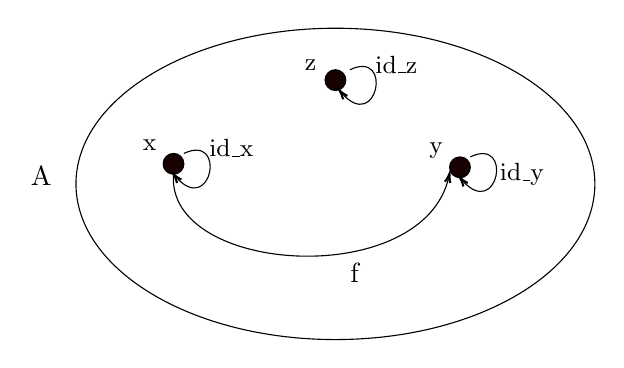
\begin{tikzpicture}[x=0.75pt,y=0.75pt,yscale=-1,xscale=1]
%uncomment if require: \path (0,300); %set diagram left start at 0, and has height of 300

%Shape: Ellipse [id:dp9346439808655433]
\draw   (220,155) .. controls (220,113.58) and (275.96,80) .. (345,80) .. controls (414.04,80) and (470,113.58) .. (470,155) .. controls (470,196.42) and (414.04,230) .. (345,230) .. controls (275.96,230) and (220,196.42) .. (220,155) -- cycle ;
%Shape: Circle [id:dp22784360669527182]
\draw  [fill={rgb, 255:red, 23; green, 1; blue, 1 }  ,fill opacity=1 ] (262,145.33) .. controls (262,142.56) and (264.24,140.33) .. (267,140.33) .. controls (269.76,140.33) and (272,142.56) .. (272,145.33) .. controls (272,148.09) and (269.76,150.33) .. (267,150.33) .. controls (264.24,150.33) and (262,148.09) .. (262,145.33) -- cycle ;
%Curve Lines [id:da27074905740711297]
\draw    (272,140.33) .. controls (292.91,130.36) and (285.32,171.14) .. (268.07,151.6) ;
\draw [shift={(267,150.33)}, rotate = 51.34] [color={rgb, 255:red, 0; green, 0; blue, 0 }  ][line width=0.75]    (4.37,-1.32) .. controls (2.78,-0.56) and (1.32,-0.12) .. (0,0) .. controls (1.32,0.12) and (2.78,0.56) .. (4.37,1.32)   ;
%Shape: Circle [id:dp9211255412324888]
\draw  [fill={rgb, 255:red, 23; green, 1; blue, 1 }  ,fill opacity=1 ] (400,147) .. controls (400,144.24) and (402.24,142) .. (405,142) .. controls (407.76,142) and (410,144.24) .. (410,147) .. controls (410,149.76) and (407.76,152) .. (405,152) .. controls (402.24,152) and (400,149.76) .. (400,147) -- cycle ;
%Curve Lines [id:da7233344958507704]
\draw    (410,142) .. controls (430.91,132.04) and (423.32,172.81) .. (406.07,153.27) ;
\draw [shift={(405,152)}, rotate = 51.34] [color={rgb, 255:red, 0; green, 0; blue, 0 }  ][line width=0.75]    (4.37,-1.32) .. controls (2.78,-0.56) and (1.32,-0.12) .. (0,0) .. controls (1.32,0.12) and (2.78,0.56) .. (4.37,1.32)   ;
%Curve Lines [id:da38568823352847637]
\draw    (267,150.33) .. controls (263.04,198.67) and (387.15,206.66) .. (399.66,151.69) ;
\draw [shift={(400,150)}, rotate = 102.82] [color={rgb, 255:red, 0; green, 0; blue, 0 }  ][line width=0.75]    (4.37,-1.32) .. controls (2.78,-0.56) and (1.32,-0.12) .. (0,0) .. controls (1.32,0.12) and (2.78,0.56) .. (4.37,1.32)   ;
%Shape: Circle [id:dp8096171242464965]
\draw  [fill={rgb, 255:red, 23; green, 1; blue, 1 }  ,fill opacity=1 ] (340,105) .. controls (340,102.24) and (342.24,100) .. (345,100) .. controls (347.76,100) and (350,102.24) .. (350,105) .. controls (350,107.76) and (347.76,110) .. (345,110) .. controls (342.24,110) and (340,107.76) .. (340,105) -- cycle ;
%Curve Lines [id:da10314349904359177]
\draw    (352,100) .. controls (372.91,90.04) and (365.32,130.81) .. (348.07,111.27) ;
\draw [shift={(347,110)}, rotate = 51.34] [color={rgb, 255:red, 0; green, 0; blue, 0 }  ][line width=0.75]    (4.37,-1.32) .. controls (2.78,-0.56) and (1.32,-0.12) .. (0,0) .. controls (1.32,0.12) and (2.78,0.56) .. (4.37,1.32)   ;

% Text Node
\draw (197,145.5) node [anchor=north west][inner sep=0.75pt]   [align=left] {A};
% Text Node
\draw (251,132.33) node [anchor=north west][inner sep=0.75pt]  [font=\small] [align=left] {x};
% Text Node
\draw (283,132.33) node [anchor=north west][inner sep=0.75pt]  [font=\small] [align=left] {id\_x};
% Text Node
\draw (389,134) node [anchor=north west][inner sep=0.75pt]  [font=\small] [align=left] {y};
% Text Node
\draw (423,144) node [anchor=north west][inner sep=0.75pt]  [font=\small] [align=left] {id\_y};
% Text Node
\draw (351,192) node [anchor=north west][inner sep=0.75pt]   [align=left] {f};
% Text Node
\draw (363,92) node [anchor=north west][inner sep=0.75pt]  [font=\small] [align=left] {id\_z};
% Text Node
\draw (329,94) node [anchor=north west][inner sep=0.75pt]  [font=\small] [align=left] {z};


\end{tikzpicture}
\caption{Example of a category A with objects x, y and z with a morphism f that goes from x to y}
\end{figure}

At the heart of category theory, we have the notion of composition. Suppose that
we have an arrow from A to B, and another arrow from B to C, then there is
necessarily another arrow that goes directly from A to C as we show in
\autoref{fig:cat-theory-composition}. We call this the composition of the first
two arrows. This is of course analogous to function composition in programming.

\begin{figure}
\centering

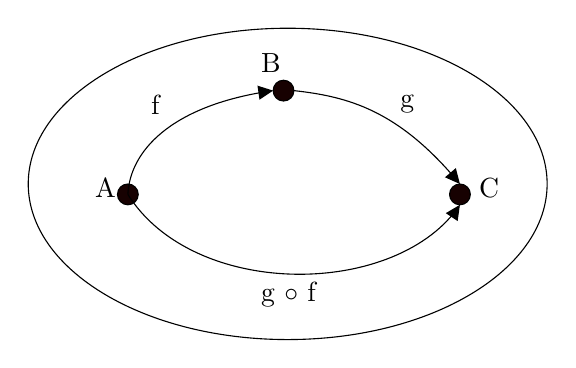
\begin{tikzpicture}[x=0.75pt,y=0.75pt,yscale=-1,xscale=1]
%uncomment if require: \path (0,300); %set diagram left start at 0, and has height of 300

%Shape: Ellipse [id:dp5682347326089148]
\draw   (210,155) .. controls (210,113.58) and (265.96,80) .. (335,80) .. controls (404.04,80) and (460,113.58) .. (460,155) .. controls (460,196.42) and (404.04,230) .. (335,230) .. controls (265.96,230) and (210,196.42) .. (210,155) -- cycle ;
%Shape: Circle [id:dp9592501831446234]
\draw  [fill={rgb, 255:red, 23; green, 1; blue, 1 }  ,fill opacity=1 ] (253,160.06) .. controls (253,157.3) and (255.24,155.06) .. (258,155.06) .. controls (260.76,155.06) and (263,157.3) .. (263,160.06) .. controls (263,162.82) and (260.76,165.06) .. (258,165.06) .. controls (255.24,165.06) and (253,162.82) .. (253,160.06) -- cycle ;
%Shape: Circle [id:dp2931536659208638]
\draw  [fill={rgb, 255:red, 23; green, 1; blue, 1 }  ,fill opacity=1 ] (328,110.06) .. controls (328,107.3) and (330.24,105.06) .. (333,105.06) .. controls (335.76,105.06) and (338,107.3) .. (338,110.06) .. controls (338,112.82) and (335.76,115.06) .. (333,115.06) .. controls (330.24,115.06) and (328,112.82) .. (328,110.06) -- cycle ;
%Curve Lines [id:da24285465512107507]
\draw    (338,110.06) .. controls (364.46,112.94) and (388.04,119.72) .. (416.27,152.99) ;
\draw [shift={(418,155.06)}, rotate = 229.87] [fill={rgb, 255:red, 0; green, 0; blue, 0 }  ][line width=0.08]  [draw opacity=0] (7.14,-3.43) -- (0,0) -- (7.14,3.43) -- cycle    ;
%Curve Lines [id:da2451569195346175]
\draw    (258,160.06) .. controls (258.98,139.48) and (278.21,117.88) .. (325.09,110.49) ;
\draw [shift={(328,110.06)}, rotate = 171.94] [fill={rgb, 255:red, 0; green, 0; blue, 0 }  ][line width=0.08]  [draw opacity=0] (7.14,-3.43) -- (0,0) -- (7.14,3.43) -- cycle    ;
%Shape: Circle [id:dp5266322522520346]
\draw  [fill={rgb, 255:red, 23; green, 1; blue, 1 }  ,fill opacity=1 ] (413,160.06) .. controls (413,157.3) and (415.24,155.06) .. (418,155.06) .. controls (420.76,155.06) and (423,157.3) .. (423,160.06) .. controls (423,162.82) and (420.76,165.06) .. (418,165.06) .. controls (415.24,165.06) and (413,162.82) .. (413,160.06) -- cycle ;
%Curve Lines [id:da19962913311880914]
\draw    (258,160.06) .. controls (289.52,210.24) and (385.07,210.02) .. (416.6,167.05) ;
\draw [shift={(418,165.06)}, rotate = 123.72] [fill={rgb, 255:red, 0; green, 0; blue, 0 }  ][line width=0.08]  [draw opacity=0] (7.14,-3.43) -- (0,0) -- (7.14,3.43) -- cycle    ;

% Text Node
\draw (321,91) node [anchor=north west][inner sep=0.75pt]   [align=left] {B};
% Text Node
\draw (241,151) node [anchor=north west][inner sep=0.75pt]   [align=left] {A};
% Text Node
\draw (426,151) node [anchor=north west][inner sep=0.75pt]   [align=left] {C};
% Text Node
\draw (268,111) node [anchor=north west][inner sep=0.75pt]   [align=left] {f};
% Text Node
\draw (388,111) node [anchor=north west][inner sep=0.75pt]   [align=left] {g};
% Text Node
\draw (321,201) node [anchor=north west][inner sep=0.75pt]   [align=left] {g $\circ$ f};

\end{tikzpicture}

\caption{The composition of two morphisms f and g. The identity arrows are not explicitly shown as we can take their existence for granted.}\label{fig:cat-theory-composition}

\end{figure}

To conclude our short introduction to category theory, we would like to present
the category-theoretic equivalent of a ubiquitous construct in type theory,
i.e.\ products (also known as tuples). One should be familiar with the notion of
products being defined as pairs of elements, however, in category theory, we have
to define such objects in terms of their morphisms that relate them to other
objects. If some object C were to be the product of objects A and B, then we
require that it has two morphisms that behave as the first and second
projections out of the product. In other words, we require the two morphisms
$\id{p} : \id{C} \rightarrow \id{A}$ and $\id{q} : \id{C} \rightarrow \id{B}$.

\begin{figure}
  \centering

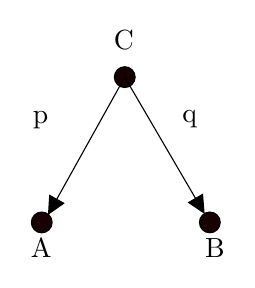
\begin{tikzpicture}[x=0.75pt,y=0.75pt,yscale=-1,xscale=1]
%uncomment if require: \path (0,300); %set diagram left start at 0, and has height of 300

%Shape: Circle [id:dp07095704485213461]
\draw  [fill={rgb, 255:red, 23; green, 1; blue, 1 }  ,fill opacity=1 ] (339.5,95.06) .. controls (339.5,92.3) and (341.74,90.06) .. (344.5,90.06) .. controls (347.26,90.06) and (349.5,92.3) .. (349.5,95.06) .. controls (349.5,97.82) and (347.26,100.06) .. (344.5,100.06) .. controls (341.74,100.06) and (339.5,97.82) .. (339.5,95.06) -- cycle ;
%Shape: Circle [id:dp6029113112328306]
\draw  [fill={rgb, 255:red, 23; green, 1; blue, 1 }  ,fill opacity=1 ] (380.5,165.06) .. controls (380.5,162.3) and (382.74,160.06) .. (385.5,160.06) .. controls (388.26,160.06) and (390.5,162.3) .. (390.5,165.06) .. controls (390.5,167.82) and (388.26,170.06) .. (385.5,170.06) .. controls (382.74,170.06) and (380.5,167.82) .. (380.5,165.06) -- cycle ;
%Shape: Circle [id:dp8272191866621565]
\draw  [fill={rgb, 255:red, 23; green, 1; blue, 1 }  ,fill opacity=1 ] (299.5,165.06) .. controls (299.5,162.3) and (301.74,160.06) .. (304.5,160.06) .. controls (307.26,160.06) and (309.5,162.3) .. (309.5,165.06) .. controls (309.5,167.82) and (307.26,170.06) .. (304.5,170.06) .. controls (301.74,170.06) and (299.5,167.82) .. (299.5,165.06) -- cycle ;
%Straight Lines [id:da6629962247946746]
\draw    (344.5,95.06) -- (308.96,158.88) ;
\draw [shift={(307.5,161.5)}, rotate = 299.11] [fill={rgb, 255:red, 0; green, 0; blue, 0 }  ][line width=0.08]  [draw opacity=0] (8.93,-4.29) -- (0,0) -- (8.93,4.29) -- cycle    ;
%Straight Lines [id:da8118877575329375]
\draw    (344.5,95.06) -- (381.49,158.41) ;
\draw [shift={(383,161)}, rotate = 239.72] [fill={rgb, 255:red, 0; green, 0; blue, 0 }  ][line width=0.08]  [draw opacity=0] (8.93,-4.29) -- (0,0) -- (8.93,4.29) -- cycle    ;

% Text Node
\draw (338,71.5) node [anchor=north west][inner sep=0.75pt]   [align=left] {C};
% Text Node
\draw (382,171.5) node [anchor=north west][inner sep=0.75pt]   [align=left] {B};
% Text Node
\draw (298,171.5) node [anchor=north west][inner sep=0.75pt]   [align=left] {A};
% Text Node
\draw (299,110.5) node [anchor=north west][inner sep=0.75pt]   [align=left] {p};
% Text Node
\draw (371,110) node [anchor=north west][inner sep=0.75pt]   [align=left] {q};

\end{tikzpicture}

\caption{A candidate product of A and B with its projection morphisms.}

\end{figure}

However, we notice that this is far too general of a definition since it is
likely that many objects fulfil these criteria. Here, we introduce the notion of
a universal property which allows us to identify \emph{the best product}. The
best product is the one that is not too general, and yet not too restrictive, it
is \emph{just right}. More formally, the product of $A$ and $B$ is an object $A
\times B$ with the morphisms $\pi_1 : A \times B \rightarrow A$ and $\pi_2 : A
\times B \rightarrow B$. Additionally, for any other object $C$ with morphisms
$p : C \rightarrow A$ and $q : C \rightarrow B$, there exists a unique morphism
$f$ such that $p = \pi_1 \circ f$ and $q = \pi_2 \circ f$. In other words, we
require that the diagram in \autoref{fig:ump-product} commute.

\begin{figure}
\centering

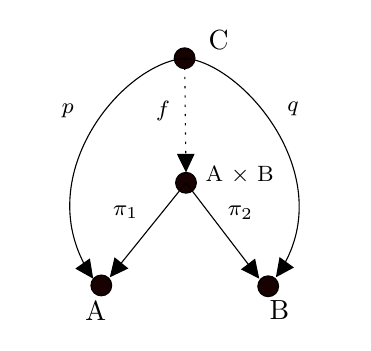
\begin{tikzpicture}[x=0.75pt,y=0.75pt,yscale=-1,xscale=1]
%uncomment if require: \path (0,300); %set diagram left start at 0, and has height of 300

%Shape: Circle [id:dp8623415585531431]
\draw  [fill={rgb, 255:red, 23; green, 1; blue, 1 }  ,fill opacity=1 ] (350.7,165.46) .. controls (350.7,162.7) and (352.94,160.46) .. (355.7,160.46) .. controls (358.46,160.46) and (360.7,162.7) .. (360.7,165.46) .. controls (360.7,168.22) and (358.46,170.46) .. (355.7,170.46) .. controls (352.94,170.46) and (350.7,168.22) .. (350.7,165.46) -- cycle ;
%Shape: Circle [id:dp8629465911347864]
\draw  [fill={rgb, 255:red, 23; green, 1; blue, 1 }  ,fill opacity=1 ] (309.9,214.92) .. controls (309.9,212.16) and (312.14,209.92) .. (314.9,209.92) .. controls (317.66,209.92) and (319.9,212.16) .. (319.9,214.92) .. controls (319.9,217.69) and (317.66,219.92) .. (314.9,219.92) .. controls (312.14,219.92) and (309.9,217.69) .. (309.9,214.92) -- cycle ;
%Shape: Circle [id:dp07686054824860356]
\draw  [fill={rgb, 255:red, 23; green, 1; blue, 1 }  ,fill opacity=1 ] (390.3,215.32) .. controls (390.3,212.56) and (392.54,210.32) .. (395.3,210.32) .. controls (398.06,210.32) and (400.3,212.56) .. (400.3,215.32) .. controls (400.3,218.09) and (398.06,220.32) .. (395.3,220.32) .. controls (392.54,220.32) and (390.3,218.09) .. (390.3,215.32) -- cycle ;
%Straight Lines [id:da5396059636931949]
\draw    (355.7,165.46) -- (320.88,208.66) ;
\draw [shift={(319,211)}, rotate = 308.86] [fill={rgb, 255:red, 0; green, 0; blue, 0 }  ][line width=0.08]  [draw opacity=0] (8.93,-4.29) -- (0,0) -- (8.93,4.29) -- cycle    ;
%Straight Lines [id:da09985777044473254]
\draw    (355.7,165.46) -- (389.18,209.28) ;
\draw [shift={(391,211.67)}, rotate = 232.62] [fill={rgb, 255:red, 0; green, 0; blue, 0 }  ][line width=0.08]  [draw opacity=0] (8.93,-4.29) -- (0,0) -- (8.93,4.29) -- cycle    ;
%Shape: Circle [id:dp44714117032868783]
\draw  [fill={rgb, 255:red, 23; green, 1; blue, 1 }  ,fill opacity=1 ] (350.03,105.46) .. controls (350.03,102.7) and (352.27,100.46) .. (355.03,100.46) .. controls (357.79,100.46) and (360.03,102.7) .. (360.03,105.46) .. controls (360.03,108.22) and (357.79,110.46) .. (355.03,110.46) .. controls (352.27,110.46) and (350.03,108.22) .. (350.03,105.46) -- cycle ;
%Curve Lines [id:da13360932709149242]
\draw    (355.03,105.46) .. controls (324.14,108.29) and (279.69,163.31) .. (309.58,209.56) ;
\draw [shift={(311,211.67)}, rotate = 235.01] [fill={rgb, 255:red, 0; green, 0; blue, 0 }  ][line width=0.08]  [draw opacity=0] (8.93,-4.29) -- (0,0) -- (8.93,4.29) -- cycle    ;
%Curve Lines [id:da35945481458004735]
\draw    (355.03,105.46) .. controls (383.24,107.63) and (430.88,163.29) .. (400.44,208.92) ;
\draw [shift={(399,211)}, rotate = 305.93] [fill={rgb, 255:red, 0; green, 0; blue, 0 }  ][line width=0.08]  [draw opacity=0] (8.93,-4.29) -- (0,0) -- (8.93,4.29) -- cycle    ;
%Straight Lines [id:da17703597924842862]
\draw  [dash pattern={on 0.84pt off 2.51pt}]  (355.03,105.46) -- (355.66,157.46) ;
\draw [shift={(355.7,160.46)}, rotate = 269.31] [fill={rgb, 255:red, 0; green, 0; blue, 0 }  ][line width=0.08]  [draw opacity=0] (8.93,-4.29) -- (0,0) -- (8.93,4.29) -- cycle    ;

% Text Node
\draw (363.87,156.33) node [anchor=north west][inner sep=0.75pt]  [font=\footnotesize] [align=left] {A $\times$ B};
% Text Node
\draw (306,221.67) node [anchor=north west][inner sep=0.75pt]   [align=left] {A};
% Text Node
\draw (394.67,221) node [anchor=north west][inner sep=0.75pt]   [align=left] {B};
% Text Node
\draw (319.33,175.33) node [anchor=north west][inner sep=0.75pt]  [font=\footnotesize] [align=left] {$\displaystyle \pi _{1}$};
% Text Node
\draw (374.67,175.6) node [anchor=north west][inner sep=0.75pt]  [font=\footnotesize] [align=left] {$\displaystyle \pi _{2}$};
% Text Node
\draw (365.33,91) node [anchor=north west][inner sep=0.75pt]   [align=left] {C};
% Text Node
\draw (294.67,126) node [anchor=north west][inner sep=0.75pt]  [font=\footnotesize] [align=left] {$\displaystyle p$};
% Text Node
\draw (403.33,125.33) node [anchor=north west][inner sep=0.75pt]  [font=\footnotesize] [align=left] {$\displaystyle q$};
% Text Node
\draw (340,124.67) node [anchor=north west][inner sep=0.75pt]  [font=\footnotesize] [align=left] {$\displaystyle f$};

\end{tikzpicture}

\caption{Universal mapping property of the product}\label{fig:ump-product}

\end{figure}

Another way of saying the above is that $h$ factorises $p$ and $q$. The
universal product, if it exists, is unique up to isomorphism. Products are not
guaranteed to exist in every category. In the category of sets, the universal
product is none other than the Cartesian product.

\section{Coequaliser}\label{sec:coequaliser}
We now introduce the notion of a coequaliser. We shall see later that
$\id{Quotient}$ acts indeed as a coequaliser, or rather coequalisers are a
generalisation of quotients. For two arrows $\oftype{f, g}{A \rightarrow B}$, a
coequaliser is an arrow $\oftype{q}{B \rightarrow Q}$ such that $qf = qg$ (we
use juxtaposition to imply composition). The universal property of the
coequaliser then dictates that for any other $Z$ and $\oftype{z}{B \rightarrow
  Z}$, if $zf = zg$, then there must exist a unique $\oftype{u}{Q \rightarrow
  Z}$ such that $uq = g$. This allows us to call $q$ \textbf{the} coequaliser of
$f$ and $g$.

\begin{figure}[H]
  \centering
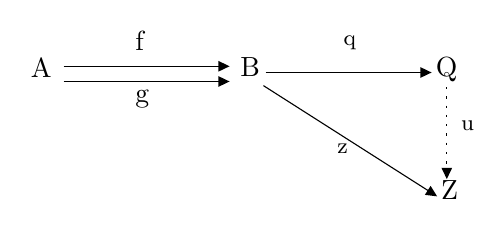
\begin{tikzpicture}[x=0.75pt,y=0.75pt,yscale=-1,xscale=1]
%uncomment if require: \path (0,300); %set diagram left start at 0, and has height of 300

%Straight Lines [id:da9967367962188358]
\draw    (208,127) -- (285,127) ;
\draw [shift={(288,127)}, rotate = 180] [fill={rgb, 255:red, 0; green, 0; blue, 0 }  ][line width=0.08]  [draw opacity=0] (5.36,-2.57) -- (0,0) -- (5.36,2.57) -- cycle    ;
%Straight Lines [id:da10808455754917401]
\draw    (208,134.33) -- (285,134.33) ;
\draw [shift={(288,134.33)}, rotate = 180] [fill={rgb, 255:red, 0; green, 0; blue, 0 }  ][line width=0.08]  [draw opacity=0] (5.36,-2.57) -- (0,0) -- (5.36,2.57) -- cycle    ;
%Straight Lines [id:da5630721975359221]
\draw    (305.33,130) -- (382.33,130) ;
\draw [shift={(385.33,130)}, rotate = 180] [fill={rgb, 255:red, 0; green, 0; blue, 0 }  ][line width=0.08]  [draw opacity=0] (5.36,-2.57) -- (0,0) -- (5.36,2.57) -- cycle    ;
%Straight Lines [id:da6026678626663149]
\draw    (304.33,136.33) -- (385.47,188.05) ;
\draw [shift={(388,189.67)}, rotate = 212.52] [fill={rgb, 255:red, 0; green, 0; blue, 0 }  ][line width=0.08]  [draw opacity=0] (5.36,-2.57) -- (0,0) -- (5.36,2.57) -- cycle    ;
%Straight Lines [id:da1216641628607622]
\draw  [dash pattern={on 0.84pt off 2.51pt}]  (392.67,137) -- (392.67,178.33) ;
\draw [shift={(392.67,181.33)}, rotate = 270] [fill={rgb, 255:red, 0; green, 0; blue, 0 }  ][line width=0.08]  [draw opacity=0] (5.36,-2.57) -- (0,0) -- (5.36,2.57) -- cycle    ;

% Text Node
\draw (191,122) node [anchor=north west][inner sep=0.75pt]  [font=\normalsize] [align=left] {A};
% Text Node
\draw (292,121.5) node [anchor=north west][inner sep=0.75pt]   [align=left] {B};
% Text Node
\draw (386.17,121.67) node [anchor=north west][inner sep=0.75pt]   [align=left] {Q};
% Text Node
\draw (388.67,181) node [anchor=north west][inner sep=0.75pt]   [align=left] {Z};
% Text Node
\draw (241.33,108.67) node [anchor=north west][inner sep=0.75pt]   [align=left] {f};
% Text Node
\draw (241.33,137.33) node [anchor=north west][inner sep=0.75pt]   [align=left] {g};
% Text Node
\draw (341.67,111) node [anchor=north west][inner sep=0.75pt]  [font=\footnotesize] [align=left] {q};
% Text Node
\draw (338.67,163) node [anchor=north west][inner sep=0.75pt]  [font=\footnotesize] [align=left] {z};
% Text Node
\draw (398.33,152) node [anchor=north west][inner sep=0.75pt]  [font=\footnotesize] [align=left] {u};


\end{tikzpicture}

\caption{Illustration of a coequaliser}

\end{figure}

\begin{prop}
In any category, if $\oftype{q}{B \rightarrow Q}$ is a coequaliser of a pair of
arrows $\oftype{f, \ g}{A \rightarrow B}$, then $q$ is an epimorphism.
\end{prop}

\begin{proof}
We first state the definition of an epimorphism. An epimorphism is a morphism $\oftype{f}{X \rightarrow Y}$ such that for all objects C and morphisms $\oftype{g_1, g_2}{Y \rightarrow Z}$, if $g_1f = g_2f$ then $g_1 = g_2$.

Now, we consider \autoref{fig:coequaliser-f-g} in which $q$ is the coequaliser of $f$ and
$g$. Supposing that $xq = yq$, we need to show that $x = y$. We have that $z =
xq = yq$, implying that $zf = xqf = xqg = zg$. By the universal property of the
coequaliser, there exists a unique $u$ such that $z = uq$. Since $z = xq$ and $z
= yq$, it must be the case that $u = x = y$. Hence, $q$ is epic.
\end{proof}

\begin{figure}
  \centering
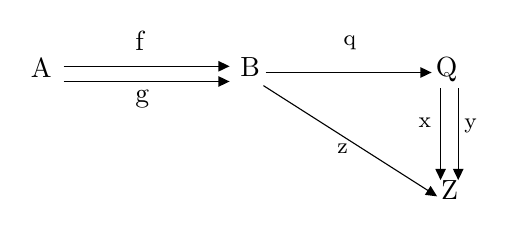
\begin{tikzpicture}[x=0.75pt,y=0.75pt,yscale=-1,xscale=1]
%uncomment if require: \path (0,300); %set diagram left start at 0, and has height of 300

%Straight Lines [id:da5779265165541632]
\draw    (208,127) -- (285,127) ;
\draw [shift={(288,127)}, rotate = 180] [fill={rgb, 255:red, 0; green, 0; blue, 0 }  ][line width=0.08]  [draw opacity=0] (5.36,-2.57) -- (0,0) -- (5.36,2.57) -- cycle    ;
%Straight Lines [id:da20539623997737722]
\draw    (208,134.33) -- (285,134.33) ;
\draw [shift={(288,134.33)}, rotate = 180] [fill={rgb, 255:red, 0; green, 0; blue, 0 }  ][line width=0.08]  [draw opacity=0] (5.36,-2.57) -- (0,0) -- (5.36,2.57) -- cycle    ;
%Straight Lines [id:da259761440148945]
\draw    (305.33,130) -- (382.33,130) ;
\draw [shift={(385.33,130)}, rotate = 180] [fill={rgb, 255:red, 0; green, 0; blue, 0 }  ][line width=0.08]  [draw opacity=0] (5.36,-2.57) -- (0,0) -- (5.36,2.57) -- cycle    ;
%Straight Lines [id:da923412514180374]
\draw    (304.33,136.33) -- (385.47,188.05) ;
\draw [shift={(388,189.67)}, rotate = 212.52] [fill={rgb, 255:red, 0; green, 0; blue, 0 }  ][line width=0.08]  [draw opacity=0] (5.36,-2.57) -- (0,0) -- (5.36,2.57) -- cycle    ;
%Straight Lines [id:da6028721128255661]
\draw    (389.67,137.5) -- (389.67,178.83) ;
\draw [shift={(389.67,181.83)}, rotate = 270] [fill={rgb, 255:red, 0; green, 0; blue, 0 }  ][line width=0.08]  [draw opacity=0] (5.36,-2.57) -- (0,0) -- (5.36,2.57) -- cycle    ;
%Straight Lines [id:da20084318131652013]
\draw    (398.17,137.5) -- (398.17,178.83) ;
\draw [shift={(398.17,181.83)}, rotate = 270] [fill={rgb, 255:red, 0; green, 0; blue, 0 }  ][line width=0.08]  [draw opacity=0] (5.36,-2.57) -- (0,0) -- (5.36,2.57) -- cycle    ;

% Text Node
\draw (191,122) node [anchor=north west][inner sep=0.75pt]  [font=\normalsize] [align=left] {A};
% Text Node
\draw (292,121.5) node [anchor=north west][inner sep=0.75pt]   [align=left] {B};
% Text Node
\draw (386.17,121.67) node [anchor=north west][inner sep=0.75pt]   [align=left] {Q};
% Text Node
\draw (388.67,181) node [anchor=north west][inner sep=0.75pt]   [align=left] {Z};
% Text Node
\draw (241.33,108.67) node [anchor=north west][inner sep=0.75pt]   [align=left] {f};
% Text Node
\draw (241.33,137.33) node [anchor=north west][inner sep=0.75pt]   [align=left] {g};
% Text Node
\draw (341.67,111) node [anchor=north west][inner sep=0.75pt]  [font=\footnotesize] [align=left] {q};
% Text Node
\draw (338.67,163) node [anchor=north west][inner sep=0.75pt]  [font=\footnotesize] [align=left] {z};
% Text Node
\draw (377.83,150.5) node [anchor=north west][inner sep=0.75pt]  [font=\footnotesize] [align=left] {x};
% Text Node
\draw (399.83,151) node [anchor=north west][inner sep=0.75pt]  [font=\footnotesize] [align=left] {y};

\end{tikzpicture}
\caption{Coequaliser diagram of morphisms $f$ and $g$}\label{fig:coequaliser-f-g}
\end{figure}



Suppose that $R$ is a pair of some set X that is related by some equivalence
relation, such that there are morphisms $\oftype{\pi_1, \pi_2}{R \rightarrow X}$
that act as projections out of the pair. Then, the projection into the quotient,
$\oftype{q}{X \rightarrow X/R}$ is an coequaliser of $\pi_1$ and $\pi_2$. Its
counterpart in Typer is the function $\id{Quotient\_in}$. Since the coequaliser
is epic, this implies that $\id{Quotient\_in}$ is surjective, as can be proven
within Typer. When we say that a function $\oftype{f}{X \rightarrow Y}$ is
surjective, we are essentially saying that $\forall y \in Y. \ \exists x \in X.
\ f(x) = y$. Note that we should represent this by a weak sum, i.e.\ we do not
require a concrete witness of $x$.

\begin{minted}[escapeinside=@@,mathescape=true]{agda}
    type SurjectiveQuotientProof (A : Type) (R : A @$\rightarrow$@ A @$\rightarrow$@ Type)
                                 (x : Quotient A R) : Type
       | surjectiveQuotientProof (a : A) (Quotient_in (R := R) a @$\equiv$@ x)
\end{minted}

We define the above type, intending to return the propositional truncation of it
as a proof of the surjectivity of $\id{Quotient\_in}$. The proof goes as
follows:

\begin{minted}[escapeinside=@@,mathescape=true]{agda}
    Quotient_in_surjective : (A : Type) @$\Rrightarrow$@ (R : A @$\rightarrow$@ A @$\rightarrow$@ Type)
                             @$\Rrightarrow$@ (x : Quotient A R)
                             @$\rightarrow$@ PropTrunc (SurjectiveQuotientProof A R x)
    Quotient_in_surjective = @$\lambda$@ A R @$\Rrightarrow$@
      elimProp (@$\lambda$@ x @$\rightarrow$@ squash (P := SurjectiveQuotientProof A R x))
               (@$\lambda$@ a @$\rightarrow$@ inPropTrunc (surjectiveQuotientProof a Eq_refl))
\end{minted}

Additionally, if we have an $\oftype{f}{X \rightarrow Y}$ such that it respects
the underlying equivalence relation, i.e. $f \circ \pi_1 = f \circ \pi_2$, then
there exists a unique function $\oftype{\overline{f}}{X/R \rightarrow Y}$ as
illustrated in \autoref{fig:coequaliser-quotient}. For $x \in X$, we have that
$f(x) = \overline{f}(q(x))$. The equivalent of $\overline{f}$ in Typer is the
function $\Funapp{\id{Quotient\_elim}}{f}{(\earg{p}{p})}$ where $p$ is an
appropriate proof that $f$ respects the relation. This also justifies the
reduction rule of \id{Quotient\_elim} which says that the application of
\id{Quotient\_elim} to some function \id{f} and an projection of some term
\id{x} into the quotient should reduce to the direct application of \id{f} to
\id{x}.

\begin{figure}
  \centering

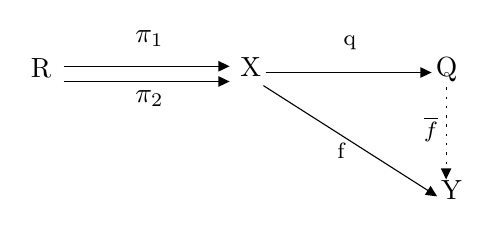
\begin{tikzpicture}[x=0.75pt,y=0.75pt,yscale=-1,xscale=1]
%uncomment if require: \path (0,300); %set diagram left start at 0, and has height of 300

%Straight Lines [id:da7734725100317463]
\draw    (228,147) -- (305,147) ;
\draw [shift={(308,147)}, rotate = 180] [fill={rgb, 255:red, 0; green, 0; blue, 0 }  ][line width=0.08]  [draw opacity=0] (5.36,-2.57) -- (0,0) -- (5.36,2.57) -- cycle    ;
%Straight Lines [id:da007971811961900777]
\draw    (228,154.33) -- (305,154.33) ;
\draw [shift={(308,154.33)}, rotate = 180] [fill={rgb, 255:red, 0; green, 0; blue, 0 }  ][line width=0.08]  [draw opacity=0] (5.36,-2.57) -- (0,0) -- (5.36,2.57) -- cycle    ;
%Straight Lines [id:da3202673895090322]
\draw    (325.33,150) -- (402.33,150) ;
\draw [shift={(405.33,150)}, rotate = 180] [fill={rgb, 255:red, 0; green, 0; blue, 0 }  ][line width=0.08]  [draw opacity=0] (5.36,-2.57) -- (0,0) -- (5.36,2.57) -- cycle    ;
%Straight Lines [id:da7225860259717922]
\draw    (324.33,156.33) -- (405.47,208.05) ;
\draw [shift={(408,209.67)}, rotate = 212.52] [fill={rgb, 255:red, 0; green, 0; blue, 0 }  ][line width=0.08]  [draw opacity=0] (5.36,-2.57) -- (0,0) -- (5.36,2.57) -- cycle    ;
%Straight Lines [id:da21057174956898383]
\draw  [dash pattern={on 0.84pt off 2.51pt}]  (412.33,157.17) -- (412.33,198.5) ;
\draw [shift={(412.33,201.5)}, rotate = 270] [fill={rgb, 255:red, 0; green, 0; blue, 0 }  ][line width=0.08]  [draw opacity=0] (5.36,-2.57) -- (0,0) -- (5.36,2.57) -- cycle    ;

% Text Node
\draw (211,142) node [anchor=north west][inner sep=0.75pt]  [font=\normalsize] [align=left] {R};
% Text Node
\draw (312,141.5) node [anchor=north west][inner sep=0.75pt]   [align=left] {X};
% Text Node
\draw (406.17,141.67) node [anchor=north west][inner sep=0.75pt]   [align=left] {Q};
% Text Node
\draw (408.67,201) node [anchor=north west][inner sep=0.75pt]   [align=left] {Y};
% Text Node
\draw (261.33,128.67) node [anchor=north west][inner sep=0.75pt]   [align=left] {$\displaystyle \pi _{1}$};
% Text Node
\draw (261.33,157.33) node [anchor=north west][inner sep=0.75pt]   [align=left] {$\displaystyle \pi _{2}$};
% Text Node
\draw (361.67,131) node [anchor=north west][inner sep=0.75pt]  [font=\footnotesize] [align=left] {q};
% Text Node
\draw (358.67,183) node [anchor=north west][inner sep=0.75pt]  [font=\footnotesize] [align=left] {f};
% Text Node
\draw (400.5,170.17) node [anchor=north west][inner sep=0.75pt]  [font=\footnotesize] [align=left] {$\overline{f}$};

\end{tikzpicture}
\caption{Coequaliser diagram of \id{Quotient}}\label{fig:coequaliser-quotient}

\end{figure}

We can also phrase the universal property of $\id{Quotient}$ in a type-theoretic
way as follows:

\begin{align*}
  & (X/R \rightarrow Y) \ \simeq \ \sum\limits_{(\oftype{f}{X \rightarrow Y})} \ (\lambda \ (x \ y : X) \rightarrow \Funapp{R}{x}{y} \rightarrow \Funapp{f}{x} \equiv \Funapp{f}{y}) \\
\end{align*}

This property says that a map between the quotient $X / R$ to some type $Y$ is
equivalent to some function of type $X \rightarrow Y$ accompanied by a
proof that the function respects the quotient. This may be proven within Typer
itself, the proof is provided in \autoref{app:ump-quot} of the appendix.

\chapter{Conclusion}

The principal objective of our work was to introduce quotient types to Typer.
We also took the opportunity to implement cubical equality in Typer, it
provides our system with a more powerful equality type by viewing equalities as
paths. The extra expressivity allows us to manipulate equalities more
conveniently and elegantly. This has also allowed us to derive functional
extensionality as a theorem, something that is not typically feasible in
intensional type theories.

We forewent the more powerful quotient inductive types in favour of classic
quotient types \latinphrase{à la} Hoffman. The implementation of our quotients
may be seen as a compromise between implementation complexity and
expressiveness. We have seen that in some cases they are not so easy to use due
to the arduous proof obligations that they impose. To some extent, our work
demonstrates that the user-friendliness of quotient types is highly dependent on
the system's support for proof development. In the case of Typer, its principal
shortcomings are the lack of tactics and the specialisation of types in case
branches. Although our quotients have their limitations, they still offer
sufficient expressivity to programmers to construct most quotients that are
interesting as far as general programming tasks are concerned. With Typer's
quotients, we have constructed illustrative examples in the form of rational
numbers and multisets. For future work, one may think of constructing other
interesting examples such as the representation of terms of the lambda calculus
such that the $\alpha$-equivalence and the $\eta$-equivalence of terms are
appropriately represented. Another example that one may construct with quotients
is the Cauchy reals as described in the HoTT book\cite[Chap. 11.3.1]{HoTTbook}.
All in all, this work was an interesting attempt to introduce extensional
concepts such as functional extensionality and quotients to a system based on
intensional type theory.

%%--------------%
%%     index    %
%%--------------%

%% S'il y a lieu, décommenter la ligne pour mettre votre index

%%\printindex

%%------------------------------------------------- %
%%         références --- bibliographie             %
%%------------------------------------------------- %

\def\bibname{References}
\bibliography{main}
\bibliographystyle{ieeetr}



%%------------------------------------------------- %
%%                  Annexe A                        %
%%------------------------------------------------- %

\anglais
\appendix

\chapter{Natural Deduction}\label{app:natural-deduction}

In this work, we use natural deduction to describe the typing rules of the
terms in our system. The typing judgements that we shall work with have the
form of $\vdash \oftype{\id{a}}{\id{A}}$, implying that the term \id{a} has the
type \id{A}. We may also include a comma-separated list of hypotheses in
judgements; they are separated from the conclusion by the turnstile ($\vdash$).
For instance, $\oftype{\oftype{\id{i}}{\id{Int}}}{\id{i + 1}}{\id{Int}}$ may be
read as ``Given that we have some \id{i} of type \id{Int}, then we deduce that
\id{i + 1} is also of type \id{Int}.''. For precision, we want our rules to
be valid under arbitrary additional hypotheses. Thus, we use the symbol $\ctx$,
known as the context, to represent an arbitrary list of hypotheses, giving us
judgements of the form $\oftype{\ctx}{\id{a}}{\id{A}}$.

When writing rules, we often want to say that a conclusion may be drawn only
when a certain number of premises are true. We do this by stating a list of
premises before stating the conclusion, with an inference line separating the
two. We illustrate this by showing the introduction rule of lambda functions.

\begin{prooftree*}
   \hypo{\oftype{\ctx, \oftype{\id{a}}{\id{A}}}{\id{b}}{\id{B}}}
   \infer1{\oftype{\ctx}{\lambda (\id{a} : \id{A}) \rightarrow \id{b}}{\id{A} \rightarrow \id{B}}}
\end{prooftree*}

The rule says that if we can deduce that $\id{b}$ has type \id{B} with the
assumption that there is some \id{a} of type \id{A} in the context, then we can
construct a function of type \fn{A $\rightarrow$ B} with
$(\oftype{\id{a}}{\id{A}})$ as its argument and \id{b} as its body.

We also show the corresponding elimination rule for functions.

\begin{prooftree*}
   \hypo{\oftype{\ctx}{\id{a}}{\id{B} \rightarrow \id{C}}}
   \hypo{\oftype{\ctx}{\id{b}}{\id{B}}}
   \infer2{\oftype{\ctx}{\Funapp{\id{a}}{\id{b}}}{\id{C}}}
\end{prooftree*}

The rule says that if we have a function \id{a} of type \fn{B $\rightarrow$ C}
as well as a term \id{b} of type \id{B}, then we can deduce that the
application of \id{a} to \id{b} is of type \id{C}.

\chapter{Reduction Rules}\label{app:reduction-rules}

To describe the evaluation of terms in our system, we use small-step
operational semantics. This allows us to show how a program executes one step
at a time. A typical reduction rule has the form of $\id{t}_1 \leadsto{}
\id{t}_2$, this may be read as ``$\id{t}_1$ reduces to $\id{t}_2$''. We provide
a concrete example by showing a reduction rule for a
\fn{\kw{if}...\kw{then}...\kw{else}} expression:

\begin{prooftree*}
  \infer0[\textsc{If-Then-Else-True}]{\kw{if} \ \id{true} \ \kw{then} \ \id{t}_1 \ \kw{else} \ \id{t}_2
                     \leadsto{} \id{t}_1}
\end{prooftree*}

This rule states that when the scrutinee of an
\fn{\kw{if}...\kw{then}...\kw{else}} expression is \id{true}, the entire
expression reduces to the term in the \kw{then} branch. A similar rule may be
written for the case where the scrutinee is \id{false}.

If the scrutinee of the \fn{\kw{if}...\kw{then}...\kw{else}} is not a canonical
value of the \id{Bool} type, i.e., if it is not \id{true} or \id{false}, then
we would not be able to apply the above rule. This is where {congruence rules}
come into the picture, they allow us to perform a step of reduction on a
sub-expression of a larger expression. We illustrate this by showing the
congruence rule for \fn{\kw{if}...\kw{then}...\kw{else}} expressions.

\begin{prooftree*}
  \hypo{\id{t}_1 \leadsto{} \id{t}_1^{'} }
  \infer1[\textsc{If-Then-Else-Cong}]{\kw{if} \ \id{t}_1 \ \kw{then} \ \id{t}_2 \ \kw{else} \ \id{t}_3
  \leadsto{} \kw{if} \ \id{t}_1^{'} \ \kw{then} \ \id{t}_2 \ \kw{else} \ \id{t}_3}
\end{prooftree*}

This rule has a premise stating that if the scrutinee, $\id{t}_1$, of an
\fn{\kw{if}...\kw{then}...\kw{else}} expression can be reduced by one step to
$\id{t}_1^{'}$ , then the entire expression can be reduced by one step to the same
expression with $\id{t}_1$  replaced by $\id{t}_1^{'}$.

\chapter{Equational Reasoning}\label{app:eq-reasoning}
Equational reasoning provides us with a neat way of expressing proofs in Typer.
With the help of some syntactic sugar, this allows us to build chains of
equality proofs by using the transitivity property of equality as shown in
Section~\ref{sec:eqtransitivity}. This is something that is implemented
in the libraries of most proof assistants, such as \Agda{}, and \Lean{}. This
allows lengthy proofs to remain readable as intermediate steps are documented
and are clearly seen.

First, we introduce a helper function that simply invokes the transitivity
property of equality proofs. This function carries out a single step of
equational reasoning.

\begin{minted}[escapeinside=@@,mathescape=true]{agda}
    step-@$\equiv$@ : (x : ?A) @$\rightarrow$@ (y : ?A) @$\rightarrow$@ (z : ?A) @$\rightarrow$@ x @$\equiv$@ y @$\rightarrow$@ y @$\equiv$@  z @$\rightarrow$@ x @$\equiv$@ z
    step-@$\equiv$@ _ p q = Eq_trans p q
\end{minted}

Next, we require a second function to conclude a chain of equational reasoning.

\begin{minted}[escapeinside=@@,mathescape=true]{agda}
    qed : (x : ?A) @$\rightarrow$@ x @$\equiv$@  x
    qed x = Eq_refl
\end{minted}

To make it all come together, we wrap the above functions with some syntactic
sugar.

\begin{minted}[escapeinside=@@,mathescape=true]{agda}
    _==<_>==_ = step-@$\equiv$@

    _@$\qed$@ = qed
\end{minted}

\verb|_==<_>==_| can be seen as a mixfix operator, whereas \_$\qed$ is a postfix
operator.

When we write the following

\begin{lstlisting}
    x
    ==< p >==
    y
    ==< ... >==
    .
    .
    .
    ==< ... >==
    z $\qed$
\end{lstlisting}

We require that $\id{p}$ be a proof of equality between $\id{x}$ and $\id{y}$,
and this can be chained \latinphrase{ad infinitum}. The expression in its
entirety is a proof of equality between $\id{x}$ and $\id{z}$. The usage of
this is best illustrated via a simple example:

\begin{minted}[escapeinside=@@,mathescape=true]{agda}
    example : (x : ?A) @$\rightarrow$@ (y : ?A) @$\rightarrow$@ (z : ?A) @$\rightarrow$@ (w : ?A)
              @$\rightarrow$@ (p : x @$\equiv$@ y) @$\rightarrow$@ (q : y @$\equiv$@ z) @$\rightarrow$@ (r : z @$\equiv$@ w) @$\rightarrow$@ x @$\equiv$@ w
    example x y z w p q r =
      x ==< p >==
      y ==< q >==
      z ==< r >==
      w @$\qed$@
\end{minted}

For a more involved example, we rewrite the proof of \verb|Integer_*DistR+|
that was shown in Section~\ref{subsec:int-theorems} by using equational
reasoning.

\begin{minted}[escapeinside=@@,mathescape=true]{agda}
    Integer_*DistR+ : (x y z : Integer) @$\rightarrow$@ x * (y + z) @$\equiv$@ (x * y) + (x * z)
    Integer_*DistR+ x y z =
      x * (y + z)
      ==< Integer_*-comm x (y + z) >==
      (y + z) * x
      ==< Integer_*DistL+ y z x >==
      (y * x) + (z * x)
      ==< Eq_cong (@$\lambda$@ e @$\rightarrow$@ e + (z * x)) (Integer_*-comm y x) >==
      (x * y) + (z * x)
      ==< Eq_cong (@$\lambda$@ e @$\rightarrow$@ (x * y) + e) (Integer_*-comm z x) >==
      (x * y) + (x * z) @$\qed$@
\end{minted}

\chapter{Other proofs}\label{app:other-proofs}

\section{Relationship between functions out of $\bI$ and equality}\label{app:proof-i->a-equiv}

We provide a proof of Theorem~\ref{theo:i->a-equiv}.

\begin{proof}
We define functions \id{f} and \id{g} as inhabitants of the forward and backward
directions of the equivalence respectively. We prove this equivalence by proving
that \fn{g} is a quasi-inverse of \fn{f} as defined in~\cite[Chap.
  2]{HoTTbook}. To this end, we define \id{f} and \id{g} as such:

\begin{align*}
  & f : (\bI \rightarrow A) \rightarrow \Sigma_{\oftype{x}{A}} . \Sigma_{\oftype{y}{A}} . \eqtype{x}{y} \\
  & f(h) := \braket{h(\ileft), \braket{h(\iright), \kw{cong}_{h}(seg)}} \\ \\
  & g : \Sigma_{\oftype{x}{A}} . \Sigma_{\oftype{y}{A}} . (\eqtype{x}{y}) \rightarrow  (\bI \rightarrow A) \\
  & g \braket{x, \braket{y, p}} := \lambda i . \ \kw{elim}_{\bI}^{A}(x, y, p, i)
\end{align*}

In order to construct $f$, we need to construct a term of type
$\Sigma_{\oftype{x}{A}} . \Sigma_{\oftype{y}{A}} . \eqtype{x}{y}$ by providing
two terms of type $A$ along with a proof that they are equal. We do so by
calling $h$ with both endpoints of $\bI$ and the congruence of equality is proof
that the two terms are equal. To construct $g$, we do the opposite by
deconstructing the term of $\Sigma_{\oftype{x}{A}} . \Sigma_{\oftype{y}{A}} .
\eqtype{x}{y}$ to construct a new function out of $\bI$. This function simply
consists of using the elimination principle of $\bI$ on the argument $i$ such
that the left endpoint maps to $x$ and the right endpoint maps to $y$; the proof
that $x \equiv y$ is precisely what we need to prove the coherence of the
elimination. Now, we need to prove that \id{g} is both the left and right
inverse of \id{f}.

To do the above, we need to introduce a few new definitions. First, we introduce
the notion of a \emph{path over a path}\cite{licata2015cubical}. Consider terms
\id{a} and \id{a'} of type \id{A} as well as an equality proof \id{p} between
them. If we had a type family \fn{P :\@ A $\rightarrow$ Type}, it would be
desirable to consider equalities between terms of type \fn{P a} and \fn{P a'}.
However, this is not possible as homogeneous equality only allows us to compare
terms of the same type. Nevertheless, we know that the types \fn{P a} and \fn{P
  a'} are propositionally equal by virtue of the path \id{p}. Hence, if we want
to equate \fn{pa :\@ P a} and \fn{pa' :\@ P a'}, we would have to
construct a path between them \textbf{over} the path \id{p}. We write the type
as \fn{pa $\equiv^{x. P \ x}_{p}$ pa'}. This may be defined in several ways, one
way is to do it in terms of normal equality as $\kw{cast}(\id{p}, \lambda \id{x}
. \id{P} \ \id{x}, \id{pa}) \equiv \id{pa'}$. By casting \id{pa} to \id{P a'},
we obtain something comparable with \id{pa'}. There is also a dependent version
of congruence on equality, \kw{congd}, which applies a dependent function to a
homogeneous equality to produce a path over it. For \fn{a a' :\@ A}, \fn{p
  :\@ a $\equiv$ a'} and \fn{f :\@ (x :\@ A) $\rightarrow$ C a}, we write
\fn{\kw{congd}$_{f}$(p) :\@ f a $\equiv^{x. C \ x}_{p}$ f a'}. We also
define the dependent eliminator \kw{elimd}$_{\bI}$ for the interval type as
follows:

\begin{prooftree*}
   \hypo{\oftype{\ctx}{C}{\bI \rightarrow Type}}
   \hypo{\oftype{\ctx}{M}{C \ \ileft}}
   \hypo{\oftype{\ctx}{N}{C \ \iright}}
   \hypo{\oftype{\ctx}{P}{M \equiv^{x . C \ x}_{seg} N}}
   \infer4{\oftype{\ctx, \oftype{i}{\bI}}{\kw{elimd}_{\bI}^{C} (M, N, P, i)}{C \ i}}
\end{prooftree*}


with the following computation rules:

\begin{align*}
  & \kw{elimd}_{\bI}^{C}(M, N, P, \ileft) \leadsto{} M \\
  & \kw{elimd}_{\bI}^{C}(M, N, P, \iright) \leadsto{} N \\
  & \kw{congd}_{\kw{elimd}_{\bI}^{C}(M, N, P)}(seg) \leadsto{} P
\end{align*}


With that, we finally have all we need to complete the proof.

\begin{align*}
  & \id{$\alpha$-helper} : (\oftype{h}{\bI \rightarrow A}) \rightarrow (\oftype{i}{\bI}) \rightarrow \eqtype{(g \ (f \ h)) \ i}{h \ i} \\
  & \id{$\alpha$-helper} \ (h , i) = \kw{depElim}_{\bI}^{i.\eqtype{(g (f \ h)) \ i}{h \ i}}(\kw{refl}_{h (\ileft)}, \ \kw{refl}_{h (\iright)}, \ \kw{congd}_{\lambda i . \kw{refl}_{h(i)}}(seg), \ i) \\
  & \alpha : (\oftype{h}{\bI \rightarrow A}) \rightarrow \eqtype{g \ (f \ h)}{h} \\
  & \alpha(h) =  \kw{funExt} (\id{$\alpha$-helper} (h)) \\ \\
  & \beta :  (\oftype{e}{\Sigma_{\oftype{x}{A}} . \Sigma_{\oftype{y}{A}} . \eqtype{x}{y}}) \rightarrow f \ (g \ (e)) \equiv e \\
  & \beta(e) =  \refl{\Sigma_{\oftype{x}{A}} . \Sigma_{\oftype{y}{A}} . \eqtype{x}{y}}{e}
\end{align*}

We define \id{$\alpha$-helper} as a lemma to help prove that $g$ is a left
inverse of $f$. To construct a proof of $\eqtype{(g (f \ h)) \ i}{h \ i}$, we
use the dependent elimination principle of $\bI$ on the argument $i$. When $i =
\ileft$, we would need to prove that $\eqtype{(g \ (f \ h)) \ \ileft}{h
  \ \ileft}$, however if we try to evaluate $(g \ (f \ h)) \ \ileft$, we realise
that this actually evaluates to $h \ \ileft$. This implies that the required
proof is trivially satisfied by reflexivity; the same thing can be done for
$\iright$. We prove that $\kw{refl}_{h (\ileft)}$ and $\kw{refl}_{h (\iright)}$
are equal using the dependent version of the congruence of equality. The partial
application of \id{$\alpha$-helper} with $h$ gives us a proof that $g(f \ h)$
and $h$ are pointwise equal, thus allowing us to invoke \kw{funExt} to get the
desired result.

To prove $\beta$, we first deconstruct $e$ to $\braket{x, \braket{y, p}}$. We
now show how the expression $f \ (g \ (e))$ gets reduced.

\begin{align*}
  & f \ (g \ \braket{x, \braket{y, p}})  \\
  & \leadsto f \ (\lambda i . \ \kw{elim}_{\bI}^{A}(x, y, p, i)) \\
  & \leadsto \braket{x, \braket{y, \kw{cong}_{\lambda i . \ \kw{elim}_{\bI}^{A}(x, y, p, i)}(seg)}} \\
  & \leadsto \braket{x, \braket{y, \kw{cong}_{\kw{elim}_{\bI}^{A}(x, y, p)}(seg)}} \\
  & \leadsto \braket{x, \braket{y, p}} \\
\end{align*}

The third reduction uses the $\eta$-equivalence of functions. As for the final
reduction, we assume that the functorial action of $\kw{elim}_{\bI}^{A}(x, y, p)$
on $seg$ computes to $p$ to simplify the proof. Given that we may reduce $f \ (g
\ \braket{x, \braket{y, p}})$ to $\braket{x, \braket{y, p}}$, they are thus
definitionally equal, allowing us to proof $\beta$ by reflexivity.\end{proof}

\section{Closure of Mere Propositions under the $\Pi$-type}\label{app:closure-mp-pi}

Consider a type \id{A} and a type family \fn{B :\@ A $\rightarrow$ Type}. If it
is the case that \fn{$\forall$ a.\ isProp (B a)}, then it is also true that
\fn{isProp ((a :\@ A) $\rightarrow$ B a)}. In other words, the property that
\fn{B a} is a mere proposition is closed under the $\Pi$ type former. We
provide a proof of this in the form of Typer code.

\begin{minted}[escapeinside=@@,mathescape=true]{agda}
isProp@$\Pi$@ : (h : (x : ?A) @$\rightarrow$@ isProp (?B x))
          @$\rightarrow$@ isProp ((x : ?A) @$\rightarrow$@ ?B x)
isProp@$\Pi$@ h f g = Eq_eq (f := @$\lambda$@ i @$\Rrightarrow$@ @$\lambda$@ (x : A) @$\rightarrow$@ Eq_uneq (p := h x (f x) (g x))
                                                         (i := i))
\end{minted}

Recall the definition of \id{isProp} stated in \autoref{sec:prop-trunc}.

\section{Whiskering}\label{app:whiskering}

We use the term whiskering to refer to the concatenation of a heterogeneous
equality with a homogeneous equality.

If we have a heterogeneous equality proof between \id{a0} and \id{a1} and a
homogeneous equality proof between \id{a1} and \id{a2}, then we can construct a
heterogeneous equality proof between \id{a0} and \id{a2} as follows:

\begin{minted}[escapeinside=@@,mathescape=true]{agda}
whiskerRight : (A : I @$\Rrightarrow$@ Type) @$\Rrightarrow$@ (a0 : A (_ := @$\ileft$@)) @$\Rightarrow$@ (a1 a2 : A (_ := @$\iright$@))
               @$\Rightarrow$@ Heq a0 a1 @$\rightarrow$@ a1 @$\equiv$@ a2 @$\rightarrow$@ Heq a0 a2
whiskerRight = @$\lambda$@ A @$\Rrightarrow$@ @$\lambda$@ a0 a1 a2 @$\Rightarrow$@ @$\lambda$@ p1 p2 @$\rightarrow$@
  Eq_cast (p := p2) (f := @$\lambda$@ x @$\rightarrow$@ Heq (t := A) a0 x) p1
\end{minted}


This is analogous to our proof of \id{Eq\_trans} in
\autoref{sec:eqtransitivity}. \id{whiskerLeft} may be defined in a similar
fashion.

\section{Properties of dependent pairs}\label{app:deppairs-properties}

In this section, we prove some theorems related to the \id{Sigma} type
introduced in \autoref{subsec:existential-sigma}. $\eta$-equivalence does not
hold definitionally for the \id{Sigma} type, however it may be proven
propositionally:

\begin{minted}[escapeinside=@@,mathescape=true]{agda}
Sigma_@$\eta$@ : (p : Sigma ?A ?P) @$\rightarrow$@ p @$\equiv$@ sigma (B := ?P) p.fst p.snd
Sigma_@$\eta$@ p = case p
    | sigma x y @$\Rightarrow$@
        let
          sigmaxy = sigma (B := P) x y

          branch=p : sigmaxy @$\equiv$@ p
          branch=p = ##DeBruijn 0

          sigmaxy_@$\eta$@ : sigmaxy @$\equiv$@ sigma (B := P) sigmaxy.fst sigmaxy.snd
          sigmaxy_@$\eta$@ = Eq_refl
        in
          Eq_cast (p := branch=p)
                  (f := @$\lambda$@ x @$\rightarrow$@ x @$\equiv$@ sigma (B := P) x.fst x.snd)
                  sigmaxy_@$\eta$@
\end{minted}

We also define a lemma, \id{$\Sigma${}$\equiv${}Prop}, which states that to
prove that two terms of type \fn{Sigma A B} are equal, if \fn{$\Pi_{x : A}$
  isProp (B x)} is true, then it suffices to show that the first projection of
the two dependent pairs are equal. The proof of this lemma is as follows:

\begin{minted}[escapeinside=@@,mathescape=true]{agda}
@$\Sigma$@@$\equiv$@prop : ((x : ?A) @$\rightarrow$@ isProp (?B x)) @$\rightarrow$@ (u v : Sigma ?A ?B)
         @$\rightarrow$@ (p : u.fst @$\equiv$@ v.fst) @$\rightarrow$@ u @$\equiv$@ v
@$\Sigma$@@$\equiv$@prop propB u v p =
  let
    h : Heq (t := @$\lambda$@ i @$\Rrightarrow$@ B (Eq_uneq (p := p) (i := i)))
            u.snd (Eq_cast (p := p) (f := B) u.snd)
    h = Heq_eq (t := @$\lambda$@ i @$\Rrightarrow$@ B (Eq_uneq (p := p) (i := i)))
               (f := @$\lambda$@ i @$\Rrightarrow$@
                      I_transp (A := @$\lambda$@ j @$\Rrightarrow$@ B (Eq_uneq (p := p) (i := I_meet i j)))
                               (r := I_not i) u.snd)

    sndv_eq : Eq_cast (p := p) (f := B) u.snd @$\equiv$@ v.snd
    sndv_eq = propB v.fst (Eq_cast (p := p) (f := B) u.snd) v.snd

    pathOver : Heq (t := @$\lambda$@ i @$\Rrightarrow$@ B (Eq_uneq (p := p) (i := i)))
                   u.snd v.snd
    pathOver = whiskerRight (A := @$\lambda$@ i @$\Rrightarrow$@ B (Eq_uneq (p := p) (i := i)))
                            h sndv_eq
    r : sigma (B := B) u.fst u.snd @$\equiv$@ sigma (B := B) v.fst v.snd
    r = Eq_eq (f := @$\lambda$@ i @$\Rrightarrow$@
                    sigma (B := B) (Eq_uneq (p := p) (i := i))
                          (Heq_uneq (t := @$\lambda$@ j @$\Rrightarrow$@
                                          B (Eq_uneq (p := p) (i := j)))
                          (p := pathOver) (i := i)))
  in
    Eq_trans (Sigma_@$\eta$@ u) (Eq_trans r (Eq_comm (Sigma_@$\eta$@ v)))
\end{minted}

The above proof makes use of the \id{whiskerRight} lemma proved in
\autoref{app:whiskering}.

\section{Proof of Quotient $\eta$-equivalences}\label{app:quotient-eta}

We prove the $\eta$-equivalences of \id{Quotient} that were mentioned in
\autoref{quot-red-rules}. The first rule we prove involves first applying the
elimination principle of \id{Quotient} followed by an application of the
introduction rule to construct a quotient term that should be equal to the
initial term that was eliminated. To realise this, we require the elimination to
be carried out with a function \id{f} that acts as a normalisation function of
sorts. \id{f} maps all terms of type \id{A} to some other term that is a
canonical representative of the equivalence class of the input term. This proof
requires the usage of the property that \id{Quotient\_in} is surjective as
described in \autoref{sec:coequaliser} to allow us to `look inside' the
quotient. The usage of this property in turn requires that the equality we are
trying to prove be a mere proposition, we fulfil this by using the axiom that
says the \id{Quotient} is a Set, i.e.\ the set truncation of \id{Quotient}.

\begin{minted}[escapeinside=@@,mathescape=true]{agda}
Quotient_eta1 : (f : ?A @$\rightarrow$@ ?A)
                @$\rightarrow$@ (h1 : (a : ?A) @$\rightarrow$@ R a (f a))
                @$\rightarrow$@ (h2 : (a a' : ?A) @$\rightarrow$@ R a a' @$\rightarrow$@ f a @$\equiv$@ f a')
                @$\rightarrow$@ (q : Quotient ?A ?R)
                @$\rightarrow$@ Quotient_in (R := ?R) (Quotient_rec f (p := h2) q) @$\equiv$@ q
Quotient_eta1 f h1 h2 q =
  propTruncRec
    (A := SurjectiveQuotientProof A R q)
    (P := Quotient_in (R := R) (Quotient_rec f (p := h2) q) @$\equiv$@ q)
    (Quotient_trunc (x := Quotient_in (R := R) (Quotient_rec f (p := h2) q))
                    (y := q))
    (@$\lambda$@ s @$\rightarrow$@ case s
      | surjectiveQuotientProof a qina@$\equiv$@q @$\Rightarrow$@
        let
          q' = Quotient_in (R := R) a
          p1 : Quotient_in (R := R) (Quotient_rec f (p := h2) q')
               @$\equiv$@ Quotient_in (R := R) (f a)
          p1 = Eq_refl %% By the @$\beta$@-rule of Quotient_elim

          p2 : Quotient_in (R := R) (f a)) @$\equiv$@ Quotient_in (R := R) a
          p2 = Eq_comm (Quotient_eq (R := R) (h1 a))

          p3 = Eq_trans p1 p2
        in
          Eq_cast (p := qina@$\equiv$@q)
                  (f := @$\lambda$@ x @$\rightarrow$@ Quotient_in (R := R) (Quotient_rec f (p := h2) x) @$\equiv$@ x)
                  p3)
    (Quotient_in_surjective q)
\end{minted}

The second rule that we would like to prove does not involve the composition
\id{Quotient\_in} with \id{Quotient\_rec}. Instead, it uses \id{Quotient\_in} as
the elimination function when calling \id{Quotient\_rec}. Intuitively speaking,
the entire operation should be equal to a no-op, i.e.\ it should return a term
equal to the quotient term that was eliminated. The proof is carried out in a
similar way to the previous proof.

\begin{minted}[escapeinside=@@,mathescape=true]{agda}
Quotient_eta2 : (q : Quotient ?A ?R)
                @$\rightarrow$@ Quotient_rec (@$\lambda$@ e @$\rightarrow$@ Quotient_in (R := ?R) e)
                                (p := @$\lambda$@ a a' r @$\rightarrow$@ Quotient_eq (R := ?R) r)
                                q
                   @$\equiv$@ q
Quotient_eta2 q =
  propTruncRec
    (A := SurjectiveQuotientProof A R q)
    (P := Quotient_rec (@$\lambda$@ e @$\rightarrow$@ Quotient_in (R := R) e)
                       (p := @$\lambda$@ a a' r @$\rightarrow$@ Quotient_eq (R := R) r)
                       q
          @$\equiv$@ q)
    (Quotient_trunc (x := Quotient_rec (@$\lambda$@ e @$\rightarrow$@ Quotient_in (R := R) e)
                           (p := @$\lambda$@ a a' r @$\rightarrow$@ Quotient_eq (R := R) r)
                           q)
                    (y := q))
    (@$\lambda$@ s @$\rightarrow$@ case s
      | surjectiveQuotientProof a qina@$\equiv$@q @$\Rightarrow$@
          Eq_cast (p := qina@$\equiv$@q)
                  (f := @$\lambda$@ x @$\rightarrow$@ Quotient_rec (@$\lambda$@ e @$\rightarrow$@ Quotient_in (R := R) e)
                                             (p := @$\lambda$@ a a' r @$\rightarrow$@ Quotient_eq (R := R) r)
                                             x
                                @$\equiv$@ x)
                  %% By the @$\beta$@-rule of Quotient_elim
                  Eq_refl)
    (Quotient_in_surjective q)
\end{minted}

\section{UMP of Quotients}\label{app:ump-quot}

In order to prove that the universal property of quotients is indeed respected by our
implementation of quotient types in Typer, we need to prove the following:

\begin{align*}
  & (X/R \rightarrow Y) \simeq \Sigma \ (X \rightarrow Y) \ (\lambda \ f \rightarrow (x \ y : X) \rightarrow \Funapp{R}{x}{y} \rightarrow \Funapp{f}{x} \equiv \Funapp{f}{y}) \\
\end{align*}

To construct the forward direction of this equivalence, the function of type
\fn{A $\rightarrow$ B} may be formed by pre-composing the function \fn{f:
  Quotient A R $\rightarrow$ B} with a projection into the quotient. The
coherence property follows naturally as a consequence of the fact that elements
of the base type that are related under the relation are \emph{equal} after
their projection into the quotient.

\begin{minted}[escapeinside=@@,mathescape=true]{agda}
    e : (Quotient ?A ?R @$\rightarrow$@ ?B)
        @$\rightarrow$@ Sigma (?A @$\rightarrow$@ ?B)
                 (@$\lambda$@ g @$\rightarrow$@ (a a' : ?A) @$\rightarrow$@ ?R a a' @$\rightarrow$@ g a @$\equiv$@ g a')
    e f = sigma (@$\lambda$@ x @$\rightarrow$@ f (Quotient_in (R := R) x))
                (@$\lambda$@ x y r @$\rightarrow$@ Eq_cong f (Quotient_eq (R := R) r))
\end{minted}

As for the reverse direction, we are required to construct a map from
\fn{Quotient A R} to \id{B}. To that end, we can simply apply the function of
type \fn{A $\rightarrow$ B} to the underlying element of the quotient.
Conceptually speaking, this function merely strips away the \id{Quotient\_in}
and may be regarded as a trivial right inverse to the pre-composition with
\id{Quotient\_in}.

\begin{minted}[escapeinside=@@,mathescape=true]{agda}
    e' : Sigma (?A @$\rightarrow$@ ?B)
               (@$\lambda$@ g @$\rightarrow$@ (a a' : ?A) @$\rightarrow$@ R a a' @$\rightarrow$@ g a @$\equiv$@ g a')
         @$\rightarrow$@ (Quotient ?A ?R @$\rightarrow$@ ?B)
    e' s = Quotient_rec (R := R) s.fst (p := s.snd)
\end{minted}

Now it remains to prove that \id{e} and \id{e'} are both left and right inverses
of each other. \fn{e' $\circ{}$ e $\equiv$ id} is proved without too much hassle
by using functional extensionality and the fact that the output type \id{B} is a
Set.

\begin{minted}[escapeinside=@@,mathescape=true]{agda}
e'e=id : isSet ?B @$\rightarrow$@ (f : Quotient ?A ?R @$\rightarrow$@ ?B) @$\rightarrow$@ e' (R := ?R) (e f) @$\equiv$@ f
e'e=id isSetB f =
  let
    p : (x : Quotient A R) @$\rightarrow$@ (f : Quotient A R @$\rightarrow$@ B)
        @$\rightarrow$@ e' (R := R) (e f) x @$\equiv$@ f x
    p x f =
      elimProp (R := R)
               (P := @$\lambda$@ x @$\rightarrow$@ e' (R := R) (e f) x @$\equiv$@ f x)
               (@$\lambda$@ x @$\rightarrow$@ isSetB (e' (R := R) (e f) x) (f x))
               (@$\lambda$@ x @$\rightarrow$@ Eq_refl (x := f (Quotient_in (R := R) x)))
               x
  in
    Eq_funext (f := e' (R := R) (e f)) (g := f) (@$\lambda$@ x @$\rightarrow$@ p x f)
\end{minted}

Although it was mentioned earlier that \id{e'} is a trivial right inverse of
\id{e}, implying that \fn{e $\circ{}$ e' $\equiv$ id} should be able to proved
by reflexivity, some limitations of Typer make this unfeasible for the moment.
One of the reasons is because the $\eta$-equivalence of \id{Sigma} does not hold
definitionally as mentioned in \autoref{app:deppairs-properties}, though it may
be proven propositionally.

Another thing that we are lacking is a proof that the dependent map induced by
\id{Quotient\_rec} and \id{Quotient\_eq} is coherent. Suppose that we had terms
\fn{x y :\@ A}, \fn{r :\@ R x y} and a function \fn{f :\@ A $\rightarrow$ B} as well as a
proof \id{p} that \id{f} respects the quotient, i.e.\ \fn{p :\@ (a :\@ A) $\rightarrow$
  (a':A) $\rightarrow$ R a a' $\rightarrow$ f a $\equiv$ f a'}. Then we could
expect the below coherence property to hold:

\begin{align*}
  & \fn{Eq\_cong (Quotient\_rec f (p := p)) (Quotient\_eq r)} \equiv \fn{p x y} \\
\end{align*}

This property does not hold definitionally in Typer, however, we could prove it
by appealing to the fact that the output type \id{B} is a \textbf{Set}. In our
proof of \fn{e $\circ{}$ e' $\equiv$ id}, we shall make use of both of the above
properties manually by invoking the \id{$\Sigma$$\equiv$prop} lemma defined in
\autoref{app:deppairs-properties}. The lemma allows us to construct a short and
elegant proof of \fn{e $\circ{}$ e' $\equiv$ id}.

\begin{minted}[escapeinside=@@,mathescape=true]{agda}
ee'=id : isSet ?B
         @$\rightarrow$@ (p : Sigma (?A @$\rightarrow$@ ?B)
                       (@$\lambda$@ g @$\rightarrow$@ (x y : ?A) @$\rightarrow$@ ?R x y @$\rightarrow$@ g x @$\equiv$@ g y))
         @$\rightarrow$@ e (e' (R := R) p) @$\equiv$@ p
ee'=id isSetB p =
  let
    propSnd g =
      isProp@$\Pi$@
        (B := @$\lambda$@ x @$\rightarrow$@ (y : A) @$\rightarrow$@ R x y @$\rightarrow$@ g x @$\equiv$@ g y)
        (@$\lambda$@ x @$\rightarrow$@ isProp@$\Pi$@
                  (B := @$\lambda$@ y @$\rightarrow$@ R x y @$\rightarrow$@ g x @$\equiv$@ g y)
                  (@$\lambda$@ y @$\rightarrow$@ isProp@$\Pi$@
                            (B := @$\lambda$@ (r : R x y) @$\rightarrow$@ g x @$\equiv$@ g y)
                            (@$\lambda$@ r @$\rightarrow$@ isSetB (g x) (g y))))
  in
    @$\Sigma$@@$\equiv$@prop
      (B := @$\lambda$@ g @$\rightarrow$@ (x : A) @$\rightarrow$@ (y : A) @$\rightarrow$@ R x y @$\rightarrow$@ g x @$\equiv$@ g y)
      propSnd
      (e (e' (R := R) p)) p Eq_refl
\end{minted}

This concludes the proof of the desired equivalence.

\chapter{More operations on the equality type}\label{app:more-eq-ops}

\section*{Interval Connections}\label{sec:interval-connections}

The operations that we defined on the interval type in
\autoref{sec:interval-manipulation} correspond to
connections\cite{cohen2016cubical} that are typically drawn as squares. Such
connections allow us to construct higher-dimensional squares from paths by
adding degeneracies, i.e.\ reflexive proofs. The \textbf{meet} operation is
notably required to prove the J-rule.

\subsection*{Meet}

Suppose that we have some proof $\fn{p}$ between terms $\fn{a}$ and $\fn{b}$,
the interval meet operation allows us to construct a square that corresponds to
the following expression:

\begin{minted}[escapeinside=@@,mathescape=true]{agda}
sq : Heq (t := @$\lambda$@ i @$\Rrightarrow$@ a @$\equiv$@ Eq_uneq (p := p) (i := i))
         (Eq_refl (_ := a)) p
sq = Heq_eq (f := @$\lambda$@ i @$\Rrightarrow$@ Eq_eq (f := @$\lambda$@ j @$\Rrightarrow$@ Eq_uneq (p := p) (i := I_meet i j)))
\end{minted}

Each dimension of an n-dimensional cube is represented by an interval variable.
In this square, the $\id{i}$ dimension goes from left to right, and the $\id{j}$
dimension goes from bottom to up. Each side of the square corresponds to some
equality proof. The top and right sides of the square are simply the original
proof $\id{p}$. The left and bottom sides of the square are fixed to be constant
paths to and from the left endpoint of the proof $\id{p}$. In other words, they
can be seen to be reflexivity proofs of $\id{a}$. This is precisely what we
meant earlier by degeneracies as such paths are trivial.

\begin{center}

\begin{tikzpicture}[x=0.75pt,y=0.75pt,yscale=-1,xscale=1]
%uncomment if require: \path (0,300); %set diagram left start at 0, and has height of 300

%Straight Lines [id:da5901241884786586]
\draw    (280.24,210.16) -- (280.24,82.66) ;
\draw [shift={(280.24,80.66)}, rotate = 90] [color={rgb, 255:red, 0; green, 0; blue, 0 }  ][line width=0.75]    (10.93,-3.29) .. controls (6.95,-1.4) and (3.31,-0.3) .. (0,0) .. controls (3.31,0.3) and (6.95,1.4) .. (10.93,3.29)   ;
%Straight Lines [id:da7023100749425399]
\draw    (430.35,210.41) -- (430.35,82.74) ;
\draw [shift={(430.35,80.74)}, rotate = 90] [color={rgb, 255:red, 0; green, 0; blue, 0 }  ][line width=0.75]    (10.93,-3.29) .. controls (6.95,-1.4) and (3.31,-0.3) .. (0,0) .. controls (3.31,0.3) and (6.95,1.4) .. (10.93,3.29)   ;
%Straight Lines [id:da5268427848389134]
\draw    (290.56,70.17) -- (418.62,70.17) ;
\draw [shift={(420.62,70.17)}, rotate = 180] [color={rgb, 255:red, 0; green, 0; blue, 0 }  ][line width=0.75]    (10.93,-3.29) .. controls (6.95,-1.4) and (3.31,-0.3) .. (0,0) .. controls (3.31,0.3) and (6.95,1.4) .. (10.93,3.29)   ;
%Straight Lines [id:da001913191488255972]
\draw    (290.56,220.6) -- (417.94,220.6) ;
\draw [shift={(419.94,220.6)}, rotate = 180] [color={rgb, 255:red, 0; green, 0; blue, 0 }  ][line width=0.75]    (10.93,-3.29) .. controls (6.95,-1.4) and (3.31,-0.3) .. (0,0) .. controls (3.31,0.3) and (6.95,1.4) .. (10.93,3.29)   ;

% Text Node
\draw (275.39,61.32) node [anchor=north west][inner sep=0.75pt]   [align=left] {a};
% Text Node
\draw (275.26,211.48) node [anchor=north west][inner sep=0.75pt]   [align=left] {a};
% Text Node
\draw (425.31,61.29) node [anchor=north west][inner sep=0.75pt]   [align=left] {b};
% Text Node
\draw (425.31,211.47) node [anchor=north west][inner sep=0.75pt]   [align=left] {a};
% Text Node
\draw (208.25,132.58) node [anchor=north west][inner sep=0.75pt]  [font=\normalsize] [align=left] {Eq\_refl a};
% Text Node
\draw (347.5,49.33) node [anchor=north west][inner sep=0.75pt]  [font=\normalsize] [align=left] {p};
% Text Node
\draw (441.75,132.42) node [anchor=north west][inner sep=0.75pt]  [font=\normalsize] [align=left] {p};
% Text Node
\draw (302.92,133) node [anchor=north west][inner sep=0.75pt]  [font=\footnotesize] [align=left] {$\displaystyle \lambda $ i \ j $\displaystyle \Rrightarrow $ p ($\displaystyle i\ \land \ j$) \\\\};
% Text Node
\draw (325.25,228.92) node [anchor=north west][inner sep=0.75pt]  [font=\normalsize] [align=left] {Eq\_refl a};

\end{tikzpicture}

\end{center}

To illustrate why the given square corresponds to the expression given above,
i.e.\ a proof that \fn{Eq\_refl (\_ := a)} is equal to \id{p}, we shall examine
each side of the square. To simplify the presentation, we shall consider \id{sq}
without the \id{Eq\_eq} constructor and the \id{Eq\_uneq} deconstructor by
treating functions out of the interval themselves as equality proofs. This
reduces \id{sq} to the following expression:

\begin{minted}[escapeinside=@@,mathescape=true]{agda}
    sq = @$\lambda$@ i @$\Rrightarrow$@ @$\lambda$@ j @$\Rrightarrow$@ p (I_meet i j)
\end{minted}

Recalling the dimensions of the squares, on the left side of the square, the
dimension $\fn{i}$ is $i_0$. So we if we fix $\fn{i}$ to be $i_0$ in $\fn{sq}$,
the resulting expression is the following, which we can reduce to the constant
path on $\fn{a}$ by using the reduction rules of $\fn{I\_meet}$ defined in
\autoref{subsubsec:interval-meet}:

\begin{minted}[escapeinside=@@,mathescape=true]{agda}
    @$\lambda$@ j @$\Rrightarrow$@ p (I_meet @$i_0$@ j)
    @$\leadsto$@ @$\lambda$@ j @$\Rrightarrow$@ p @$i_0$@
    @$\leadsto$@ @$\lambda$@ j @$\Rrightarrow$@ a
    @$\leadsto$@ Eq_refl (_ := a)
\end{minted}

For the bottom side, we fix $\fn{j}$ to be $i_0$ to obtain the below expression,
which is once again a constant path on $\fn{a}$.

\begin{minted}[escapeinside=@@,mathescape=true]{agda}
    @$\lambda$@ i @$\Rrightarrow$@ p (I_meet i @$i_0$@)
    @$\leadsto$@ @$\lambda$@ i @$\Rrightarrow$@ p @$i_0$@
    @$\leadsto$@ Eq_refl (_ := a)
\end{minted}

The right side requires us to fix $\fn{i}$ to be $i_1$, giving us the below
expression which simply reduces to $\fn{p}$.

\begin{minted}[escapeinside=@@,mathescape=true]{agda}
    @$\lambda$@ j @$\Rrightarrow$@ p (I_meet @$i_1$@ j)
    @$\leadsto$@ @$\lambda$@ j @$\Rrightarrow$@ p j
    @$\leadsto$@ p
\end{minted}

By fixing $\fn{j}$ to be $i_1$, we get the expression that corresponds to the top side, which also reduces to $\fn{p}$.

\begin{minted}[escapeinside=@@,mathescape=true]{agda}
    @$\lambda$@ i @$\Rrightarrow$@ p (I_meet i @$i_1$@)
    @$\leadsto$@ @$\lambda$@ i @$\Rrightarrow$@ p i
    @$\leadsto$@ p
\end{minted}

With that, we may complete the definition of \id{eqUnique} mentioned in
\autoref{subsec:j-rule}.

\begin{minted}[escapeinside=@@,mathescape=true]{agda}
    eqUnique a b p = Eq_eq (f := @$\lambda$@ i @$\Rrightarrow$@
                              < Eq_uneq (p := p) (i := i),
                                Heq_uneq (p := sq) (i := i) >)
\end{minted}


\subsection*{Join}

The join operator allows us to construct a square similar to the one seen in the
previous section. Here, we get a proof of equality between \id{p} and \fn{Eq_refl
  (_ := b)}.

\begin{minted}[escapeinside=@@,mathescape=true]{agda}
sq : Heq (t := @$\lambda$@ i @$\Rrightarrow$@ Eq_uneq (p := p) (i := i) @$\equiv$@ b)
         p (Eq_refl (_ := b))
sq = Heq_eq (f := @$\lambda$@ i @$\Rrightarrow$@ Eq_eq (f := @$\lambda$@ j @$\Rrightarrow$@ Eq_uneq (p := p) (i := I_join i j)))
\end{minted}

We allow the reader to convince himself that the following square corresponds to
the above expression using the same method of reasoning that was employed in the
previous section.

\begin{center}
\begin{tikzpicture}[x=0.75pt,y=0.75pt,yscale=-1,xscale=1]
%uncomment if require: \path (0,300); %set diagram left start at 0, and has height of 300

%Straight Lines [id:da9309220801708125]
\draw    (280.24,210.16) -- (280.24,82.66) ;
\draw [shift={(280.24,80.66)}, rotate = 90] [color={rgb, 255:red, 0; green, 0; blue, 0 }  ][line width=0.75]    (10.93,-3.29) .. controls (6.95,-1.4) and (3.31,-0.3) .. (0,0) .. controls (3.31,0.3) and (6.95,1.4) .. (10.93,3.29)   ;
%Straight Lines [id:da27005901742474503]
\draw    (430.35,210.41) -- (430.35,82.74) ;
\draw [shift={(430.35,80.74)}, rotate = 90] [color={rgb, 255:red, 0; green, 0; blue, 0 }  ][line width=0.75]    (10.93,-3.29) .. controls (6.95,-1.4) and (3.31,-0.3) .. (0,0) .. controls (3.31,0.3) and (6.95,1.4) .. (10.93,3.29)   ;
%Straight Lines [id:da12122758686551816]
\draw    (290.56,70.17) -- (418.62,70.17) ;
\draw [shift={(420.62,70.17)}, rotate = 180] [color={rgb, 255:red, 0; green, 0; blue, 0 }  ][line width=0.75]    (10.93,-3.29) .. controls (6.95,-1.4) and (3.31,-0.3) .. (0,0) .. controls (3.31,0.3) and (6.95,1.4) .. (10.93,3.29)   ;
%Straight Lines [id:da6877885955483964]
\draw    (290.56,220.6) -- (417.94,220.6) ;
\draw [shift={(419.94,220.6)}, rotate = 180] [color={rgb, 255:red, 0; green, 0; blue, 0 }  ][line width=0.75]    (10.93,-3.29) .. controls (6.95,-1.4) and (3.31,-0.3) .. (0,0) .. controls (3.31,0.3) and (6.95,1.4) .. (10.93,3.29)   ;

% Text Node
\draw (275.39,61.32) node [anchor=north west][inner sep=0.75pt]   [align=left] {b};
% Text Node
\draw (275.26,211.48) node [anchor=north west][inner sep=0.75pt]   [align=left] {a};
% Text Node
\draw (425.31,61.29) node [anchor=north west][inner sep=0.75pt]   [align=left] {b};
% Text Node
\draw (425.31,211.47) node [anchor=north west][inner sep=0.75pt]   [align=left] {b};
% Text Node
\draw (253.25,132.58) node [anchor=north west][inner sep=0.75pt]  [font=\normalsize] [align=left] {p};
% Text Node
\draw (324.5,50.33) node [anchor=north west][inner sep=0.75pt]  [font=\normalsize] [align=left] {Eq\_refl b};
% Text Node
\draw (441.75,132.42) node [anchor=north west][inner sep=0.75pt]  [font=\normalsize] [align=left] {Eq\_refl b};
% Text Node
\draw (302.92,133) node [anchor=north west][inner sep=0.75pt]  [font=\footnotesize] [align=left] {$\displaystyle \lambda $ i \ j $\displaystyle \Rrightarrow $ p ($\displaystyle i\ \lor \ j$) \\\\};
% Text Node
\draw (349.25,225.92) node [anchor=north west][inner sep=0.75pt]  [font=\normalsize] [align=left] {p};

\end{tikzpicture}
\end{center}

\end{document}

\endinput
%%
%% End of file `gabaritmem.tex'.
